\documentclass[twoside]{book}

% Packages required by doxygen
\usepackage{fixltx2e}
\usepackage{calc}
\usepackage{doxygen}
\usepackage[export]{adjustbox} % also loads graphicx
\usepackage{graphicx}
\usepackage[utf8]{inputenc}
\usepackage{makeidx}
\usepackage{multicol}
\usepackage{multirow}
\PassOptionsToPackage{warn}{textcomp}
\usepackage{textcomp}
\usepackage[nointegrals]{wasysym}
\usepackage[table]{xcolor}

% Font selection
\usepackage[T1]{fontenc}
\usepackage[scaled=.90]{helvet}
\usepackage{courier}
\usepackage{amssymb}
\usepackage{sectsty}
\renewcommand{\familydefault}{\sfdefault}
\allsectionsfont{%
  \fontseries{bc}\selectfont%
  \color{darkgray}%
}
\renewcommand{\DoxyLabelFont}{%
  \fontseries{bc}\selectfont%
  \color{darkgray}%
}
\newcommand{\+}{\discretionary{\mbox{\scriptsize$\hookleftarrow$}}{}{}}

% Page & text layout
\usepackage{geometry}
\geometry{%
  a4paper,%
  top=2.5cm,%
  bottom=2.5cm,%
  left=2.5cm,%
  right=2.5cm%
}
\tolerance=750
\hfuzz=15pt
\hbadness=750
\setlength{\emergencystretch}{15pt}
\setlength{\parindent}{0cm}
\setlength{\parskip}{3ex plus 2ex minus 2ex}
\makeatletter
\renewcommand{\paragraph}{%
  \@startsection{paragraph}{4}{0ex}{-1.0ex}{1.0ex}{%
    \normalfont\normalsize\bfseries\SS@parafont%
  }%
}
\renewcommand{\subparagraph}{%
  \@startsection{subparagraph}{5}{0ex}{-1.0ex}{1.0ex}{%
    \normalfont\normalsize\bfseries\SS@subparafont%
  }%
}
\makeatother

% Headers & footers
\usepackage{fancyhdr}
\pagestyle{fancyplain}
\fancyhead[LE]{\fancyplain{}{\bfseries\thepage}}
\fancyhead[CE]{\fancyplain{}{}}
\fancyhead[RE]{\fancyplain{}{\bfseries\leftmark}}
\fancyhead[LO]{\fancyplain{}{\bfseries\rightmark}}
\fancyhead[CO]{\fancyplain{}{}}
\fancyhead[RO]{\fancyplain{}{\bfseries\thepage}}
\fancyfoot[LE]{\fancyplain{}{}}
\fancyfoot[CE]{\fancyplain{}{}}
\fancyfoot[RE]{\fancyplain{}{\bfseries\scriptsize Generated by Doxygen }}
\fancyfoot[LO]{\fancyplain{}{\bfseries\scriptsize Generated by Doxygen }}
\fancyfoot[CO]{\fancyplain{}{}}
\fancyfoot[RO]{\fancyplain{}{}}
\renewcommand{\footrulewidth}{0.4pt}
\renewcommand{\chaptermark}[1]{%
  \markboth{#1}{}%
}
\renewcommand{\sectionmark}[1]{%
  \markright{\thesection\ #1}%
}

% Indices & bibliography
\usepackage{natbib}
\usepackage[titles]{tocloft}
\setcounter{tocdepth}{3}
\setcounter{secnumdepth}{5}
\makeindex

% Hyperlinks (required, but should be loaded last)
\usepackage{ifpdf}
\ifpdf
  \usepackage[pdftex,pagebackref=true]{hyperref}
\else
  \usepackage[ps2pdf,pagebackref=true]{hyperref}
\fi
\hypersetup{%
  colorlinks=true,%
  linkcolor=blue,%
  citecolor=blue,%
  unicode%
}

% Custom commands
\newcommand{\clearemptydoublepage}{%
  \newpage{\pagestyle{empty}\cleardoublepage}%
}

\usepackage{caption}
\captionsetup{labelsep=space,justification=centering,font={bf},singlelinecheck=off,skip=4pt,position=top}

%===== C O N T E N T S =====

\begin{document}

% Titlepage & ToC
\hypersetup{pageanchor=false,
             bookmarksnumbered=true,
             pdfencoding=unicode
            }
\pagenumbering{alph}
\begin{titlepage}
\vspace*{7cm}
\begin{center}%
{\Large spmv }\\
\vspace*{1cm}
{\large Generated by Doxygen 1.8.13}\\
\end{center}
\end{titlepage}
\clearemptydoublepage
\pagenumbering{roman}
\tableofcontents
\clearemptydoublepage
\pagenumbering{arabic}
\hypersetup{pageanchor=true}

%--- Begin generated contents ---
\chapter{Build}
\label{md__home_tau_public_html_lecture_parallel_distributed_2018_handson_tau_parallel-distributed-handson_03spmv_README}
\Hypertarget{md__home_tau_public_html_lecture_parallel_distributed_2018_handson_tau_parallel-distributed-handson_03spmv_README}
\input{md__home_tau_public_html_lecture_parallel_distributed_2018_handson_tau_parallel-distributed-handson_03spmv_README}
\chapter{Class Index}
\section{Class List}
Here are the classes, structs, unions and interfaces with brief descriptions\+:\begin{DoxyCompactList}
\item\contentsline{section}{\hyperlink{structcmdline__options__t}{cmdline\+\_\+options\+\_\+t} \\*Command line option }{\pageref{structcmdline__options__t}}{}
\item\contentsline{section}{\hyperlink{structcoo__elem__t}{coo\+\_\+elem\+\_\+t} \\*Element of coordinate list (i, j, a) }{\pageref{structcoo__elem__t}}{}
\item\contentsline{section}{\hyperlink{structcoo__t}{coo\+\_\+t} \\*Sparse matrix in coodinate list format }{\pageref{structcoo__t}}{}
\item\contentsline{section}{\hyperlink{structcsr__elem__t}{csr\+\_\+elem\+\_\+t} \\*Element of compressed sparse row }{\pageref{structcsr__elem__t}}{}
\item\contentsline{section}{\hyperlink{structcsr__t}{csr\+\_\+t} \\*Sparse matrix in compressed row format }{\pageref{structcsr__t}}{}
\item\contentsline{section}{\hyperlink{structidx__pair__t}{idx\+\_\+pair\+\_\+t} \\*Pair of two indices (i and j) }{\pageref{structidx__pair__t}}{}
\item\contentsline{section}{\hyperlink{structsparse__format__table__entry__t}{sparse\+\_\+format\+\_\+table\+\_\+entry\+\_\+t} \\*Pair of the index value (sparse\+\_\+format\+\_\+t) and its name }{\pageref{structsparse__format__table__entry__t}}{}
\item\contentsline{section}{\hyperlink{structsparse__format__table__t}{sparse\+\_\+format\+\_\+table\+\_\+t} \\*Table of sparse format and their names }{\pageref{structsparse__format__table__t}}{}
\item\contentsline{section}{\hyperlink{structsparse__matrix__type__table__entry__t}{sparse\+\_\+matrix\+\_\+type\+\_\+table\+\_\+entry\+\_\+t} \\*Pair of the index value (matrix\+\_\+type\+\_\+t) and its name }{\pageref{structsparse__matrix__type__table__entry__t}}{}
\item\contentsline{section}{\hyperlink{structsparse__matrix__type__table__t}{sparse\+\_\+matrix\+\_\+type\+\_\+table\+\_\+t} \\*Table of sparse matrix types and their names }{\pageref{structsparse__matrix__type__table__t}}{}
\item\contentsline{section}{\hyperlink{structsparse__t}{sparse\+\_\+t} \\*Sparse matrix (in any format) }{\pageref{structsparse__t}}{}
\item\contentsline{section}{\hyperlink{structspmv__algo__table__entry__t}{spmv\+\_\+algo\+\_\+table\+\_\+entry\+\_\+t} \\*Pair of the index value (spmv\+\_\+algo\+\_\+t) and its name }{\pageref{structspmv__algo__table__entry__t}}{}
\item\contentsline{section}{\hyperlink{structspmv__algo__table__t}{spmv\+\_\+algo\+\_\+table\+\_\+t} \\*Table of spmv algorithms and their names }{\pageref{structspmv__algo__table__t}}{}
\item\contentsline{section}{\hyperlink{structvec__t}{vec\+\_\+t} \\*Vector }{\pageref{structvec__t}}{}
\end{DoxyCompactList}

\chapter{File Index}
\section{File List}
Here is a list of all documented files with brief descriptions\+:\begin{DoxyCompactList}
\item\contentsline{section}{/home/tau/public\+\_\+html/lecture/parallel\+\_\+distributed/2018/handson/tau/parallel-\/distributed-\/handson/03spmv/\hyperlink{spmv_8cc}{spmv.\+cc} \\*Sparse matrix vector multiplication }{\pageref{spmv_8cc}}{}
\item\contentsline{section}{/home/tau/public\+\_\+html/lecture/parallel\+\_\+distributed/2018/handson/tau/parallel-\/distributed-\/handson/03spmv/include/\hyperlink{coo__to__dev_8cc}{coo\+\_\+to\+\_\+dev.\+cc} \\*Make a deivce copy of a sparse matrix in coo format }{\pageref{coo__to__dev_8cc}}{}
\item\contentsline{section}{/home/tau/public\+\_\+html/lecture/parallel\+\_\+distributed/2018/handson/tau/parallel-\/distributed-\/handson/03spmv/include/\hyperlink{csr__to__dev_8cc}{csr\+\_\+to\+\_\+dev.\+cc} \\*Make a deivce copy of a sparse matrix in csr format }{\pageref{csr__to__dev_8cc}}{}
\item\contentsline{section}{/home/tau/public\+\_\+html/lecture/parallel\+\_\+distributed/2018/handson/tau/parallel-\/distributed-\/handson/03spmv/include/\hyperlink{cuda__util_8h}{cuda\+\_\+util.\+h} \\*Small utility functions for cuda }{\pageref{cuda__util_8h}}{}
\item\contentsline{section}{/home/tau/public\+\_\+html/lecture/parallel\+\_\+distributed/2018/handson/tau/parallel-\/distributed-\/handson/03spmv/include/\hyperlink{scalar__vec__cuda_8cc}{scalar\+\_\+vec\+\_\+cuda.\+cc} \\*Scalar x vector multiply with cuda }{\pageref{scalar__vec__cuda_8cc}}{}
\item\contentsline{section}{/home/tau/public\+\_\+html/lecture/parallel\+\_\+distributed/2018/handson/tau/parallel-\/distributed-\/handson/03spmv/include/\hyperlink{scalar__vec__parallel_8cc}{scalar\+\_\+vec\+\_\+parallel.\+cc} \\*Scalar x vector multiply with parallel for }{\pageref{scalar__vec__parallel_8cc}}{}
\item\contentsline{section}{/home/tau/public\+\_\+html/lecture/parallel\+\_\+distributed/2018/handson/tau/parallel-\/distributed-\/handson/03spmv/include/\hyperlink{scalar__vec__task_8cc}{scalar\+\_\+vec\+\_\+task.\+cc} \\*Scalar x vector multiply with tasks }{\pageref{scalar__vec__task_8cc}}{}
\item\contentsline{section}{/home/tau/public\+\_\+html/lecture/parallel\+\_\+distributed/2018/handson/tau/parallel-\/distributed-\/handson/03spmv/include/\hyperlink{scalar__vec__udr_8cc}{scalar\+\_\+vec\+\_\+udr.\+cc} \\*Scalar x vector multiply with parallel for + user-\/defined reductions }{\pageref{scalar__vec__udr_8cc}}{}
\item\contentsline{section}{/home/tau/public\+\_\+html/lecture/parallel\+\_\+distributed/2018/handson/tau/parallel-\/distributed-\/handson/03spmv/include/\hyperlink{spmv__coo__cuda_8cc}{spmv\+\_\+coo\+\_\+cuda.\+cc} \\*Y = A $\ast$ x for coo with cuda }{\pageref{spmv__coo__cuda_8cc}}{}
\item\contentsline{section}{/home/tau/public\+\_\+html/lecture/parallel\+\_\+distributed/2018/handson/tau/parallel-\/distributed-\/handson/03spmv/include/\hyperlink{spmv__coo__parallel_8cc}{spmv\+\_\+coo\+\_\+parallel.\+cc} \\*Y = A $\ast$ x for coo with parallel for }{\pageref{spmv__coo__parallel_8cc}}{}
\item\contentsline{section}{/home/tau/public\+\_\+html/lecture/parallel\+\_\+distributed/2018/handson/tau/parallel-\/distributed-\/handson/03spmv/include/\hyperlink{spmv__coo__sorted__cuda_8cc}{spmv\+\_\+coo\+\_\+sorted\+\_\+cuda.\+cc} \\*Y = A $\ast$ x for coo\+\_\+sorted with cuda }{\pageref{spmv__coo__sorted__cuda_8cc}}{}
\item\contentsline{section}{/home/tau/public\+\_\+html/lecture/parallel\+\_\+distributed/2018/handson/tau/parallel-\/distributed-\/handson/03spmv/include/\hyperlink{spmv__coo__sorted__parallel_8cc}{spmv\+\_\+coo\+\_\+sorted\+\_\+parallel.\+cc} \\*Y = A $\ast$ x for coo\+\_\+sorted with parallel for }{\pageref{spmv__coo__sorted__parallel_8cc}}{}
\item\contentsline{section}{/home/tau/public\+\_\+html/lecture/parallel\+\_\+distributed/2018/handson/tau/parallel-\/distributed-\/handson/03spmv/include/\hyperlink{spmv__coo__sorted__task_8cc}{spmv\+\_\+coo\+\_\+sorted\+\_\+task.\+cc} \\*Y = A $\ast$ x with tasks for coo\+\_\+sorted }{\pageref{spmv__coo__sorted__task_8cc}}{}
\item\contentsline{section}{/home/tau/public\+\_\+html/lecture/parallel\+\_\+distributed/2018/handson/tau/parallel-\/distributed-\/handson/03spmv/include/\hyperlink{spmv__coo__sorted__udr_8cc}{spmv\+\_\+coo\+\_\+sorted\+\_\+udr.\+cc} \\*Y = A $\ast$ x for coo\+\_\+sorted with parallel for + user-\/defined reductions }{\pageref{spmv__coo__sorted__udr_8cc}}{}
\item\contentsline{section}{/home/tau/public\+\_\+html/lecture/parallel\+\_\+distributed/2018/handson/tau/parallel-\/distributed-\/handson/03spmv/include/\hyperlink{spmv__coo__task_8cc}{spmv\+\_\+coo\+\_\+task.\+cc} \\*Y = A $\ast$ x for coo with tasks }{\pageref{spmv__coo__task_8cc}}{}
\item\contentsline{section}{/home/tau/public\+\_\+html/lecture/parallel\+\_\+distributed/2018/handson/tau/parallel-\/distributed-\/handson/03spmv/include/\hyperlink{spmv__coo__udr_8cc}{spmv\+\_\+coo\+\_\+udr.\+cc} \\*Y = A $\ast$ x for coo with parallel for + user-\/defined reductions }{\pageref{spmv__coo__udr_8cc}}{}
\item\contentsline{section}{/home/tau/public\+\_\+html/lecture/parallel\+\_\+distributed/2018/handson/tau/parallel-\/distributed-\/handson/03spmv/include/\hyperlink{spmv__csr__cuda_8cc}{spmv\+\_\+csr\+\_\+cuda.\+cc} \\*Y = A $\ast$ x for csr with cuda }{\pageref{spmv__csr__cuda_8cc}}{}
\item\contentsline{section}{/home/tau/public\+\_\+html/lecture/parallel\+\_\+distributed/2018/handson/tau/parallel-\/distributed-\/handson/03spmv/include/\hyperlink{spmv__csr__parallel_8cc}{spmv\+\_\+csr\+\_\+parallel.\+cc} \\*Y = A $\ast$ x for csr with parallel for }{\pageref{spmv__csr__parallel_8cc}}{}
\item\contentsline{section}{/home/tau/public\+\_\+html/lecture/parallel\+\_\+distributed/2018/handson/tau/parallel-\/distributed-\/handson/03spmv/include/\hyperlink{spmv__csr__task_8cc}{spmv\+\_\+csr\+\_\+task.\+cc} \\*Y = A $\ast$ x for csr with tasks }{\pageref{spmv__csr__task_8cc}}{}
\item\contentsline{section}{/home/tau/public\+\_\+html/lecture/parallel\+\_\+distributed/2018/handson/tau/parallel-\/distributed-\/handson/03spmv/include/\hyperlink{spmv__csr__udr_8cc}{spmv\+\_\+csr\+\_\+udr.\+cc} \\*Y = A $\ast$ x for csr with parallel for + user-\/defined functions }{\pageref{spmv__csr__udr_8cc}}{}
\item\contentsline{section}{/home/tau/public\+\_\+html/lecture/parallel\+\_\+distributed/2018/handson/tau/parallel-\/distributed-\/handson/03spmv/include/\hyperlink{vec__norm2__cuda_8cc}{vec\+\_\+norm2\+\_\+cuda.\+cc} \\*Device procedure to do vec\+\_\+norm2 on the device }{\pageref{vec__norm2__cuda_8cc}}{}
\item\contentsline{section}{/home/tau/public\+\_\+html/lecture/parallel\+\_\+distributed/2018/handson/tau/parallel-\/distributed-\/handson/03spmv/include/\hyperlink{vec__norm2__parallel_8cc}{vec\+\_\+norm2\+\_\+parallel.\+cc} \\*Square norm of a vector in serial }{\pageref{vec__norm2__parallel_8cc}}{}
\item\contentsline{section}{/home/tau/public\+\_\+html/lecture/parallel\+\_\+distributed/2018/handson/tau/parallel-\/distributed-\/handson/03spmv/include/\hyperlink{vec__norm2__task_8cc}{vec\+\_\+norm2\+\_\+task.\+cc} \\*Square norm of a vector in serial }{\pageref{vec__norm2__task_8cc}}{}
\item\contentsline{section}{/home/tau/public\+\_\+html/lecture/parallel\+\_\+distributed/2018/handson/tau/parallel-\/distributed-\/handson/03spmv/include/\hyperlink{vec__norm2__udr_8cc}{vec\+\_\+norm2\+\_\+udr.\+cc} \\*Square norm of a vector in parallel using user-\/defined reduction }{\pageref{vec__norm2__udr_8cc}}{}
\item\contentsline{section}{/home/tau/public\+\_\+html/lecture/parallel\+\_\+distributed/2018/handson/tau/parallel-\/distributed-\/handson/03spmv/include/\hyperlink{vec__to__dev_8cc}{vec\+\_\+to\+\_\+dev.\+cc} \\*Make a deivce copy of a vector }{\pageref{vec__to__dev_8cc}}{}
\end{DoxyCompactList}

\chapter{Class Documentation}
\hypertarget{structcmdline__options__t}{}\section{cmdline\+\_\+options\+\_\+t Struct Reference}
\label{structcmdline__options__t}\index{cmdline\+\_\+options\+\_\+t@{cmdline\+\_\+options\+\_\+t}}


command line option  


\subsection*{Public Attributes}
\begin{DoxyCompactItemize}
\item 
\hyperlink{spmv_8cc_a8e93478a00e685bea5e6a3f617bf03a3}{idx\+\_\+t} \hyperlink{structcmdline__options__t_aeb40f98dbcd53dc727b1d7dbb566924f}{M}
\item 
\hyperlink{spmv_8cc_a8e93478a00e685bea5e6a3f617bf03a3}{idx\+\_\+t} \hyperlink{structcmdline__options__t_aa58f87808071259b5aa8f17c64bf2960}{N}
\item 
\hyperlink{spmv_8cc_a8e93478a00e685bea5e6a3f617bf03a3}{idx\+\_\+t} \hyperlink{structcmdline__options__t_aec8f7846348926cda6d62023f62d0d25}{nnz}
\item 
long \hyperlink{structcmdline__options__t_acb60cada2976487316be88bf4309e7d6}{repeat}
\item 
char $\ast$ \hyperlink{structcmdline__options__t_a16fe2748dfda1fc639d7e3321eb0e4a9}{format\+\_\+str}
\item 
\hyperlink{spmv_8cc_a8c0094893526c01b430903b2d9227256}{sparse\+\_\+format\+\_\+t} \hyperlink{structcmdline__options__t_af8a99d8cdebe0bc5fd512d2254727231}{format}
\item 
char $\ast$ \hyperlink{structcmdline__options__t_a1669264b4602341b949007ca4336dfc2}{matrix\+\_\+type\+\_\+str}
\item 
\hyperlink{spmv_8cc_a43a568fb26bc32aeaad07769cc524c45}{sparse\+\_\+matrix\+\_\+type\+\_\+t} \hyperlink{structcmdline__options__t_abc77475ac02e2e93b9f978ea22cb6244}{matrix\+\_\+type}
\item 
char $\ast$ \hyperlink{structcmdline__options__t_ae8ab407cdc87a30c1b4cdf6b424c8370}{algo\+\_\+str}
\item 
\hyperlink{spmv_8cc_ad2cf0493af54bf76c5be68b4634fcab7}{spmv\+\_\+algo\+\_\+t} \hyperlink{structcmdline__options__t_afddf83f65e6e4a14761d84a5e876e6ac}{algo}
\item 
char $\ast$ \hyperlink{structcmdline__options__t_a2db02208284cd9664c88e6f0e7140d6d}{coo\+\_\+file}
\item 
char $\ast$ \hyperlink{structcmdline__options__t_a4ae2cfd5fda7a25e302fff37c1201f93}{rmat\+\_\+str}
\item 
double \hyperlink{structcmdline__options__t_a60e05c62d3fd439c03fd26d9f8078a4b}{rmat} \mbox{[}2\mbox{]}\mbox{[}2\mbox{]}
\item 
char $\ast$ \hyperlink{structcmdline__options__t_aa4b96337328846dd1d2c0ca8eee7933f}{dump}
\item 
long \hyperlink{structcmdline__options__t_a8034ee34658dd09267c9bdbd53050c9a}{dump\+\_\+points}
\item 
long \hyperlink{structcmdline__options__t_afa92e5953f8c49714b09ccdd12a1f8a7}{dump\+\_\+seed}
\item 
long \hyperlink{structcmdline__options__t_a065412d7cdc54cdae630389c3fda266e}{seed}
\item 
int \hyperlink{structcmdline__options__t_a25f9087b240da0b93a4295fa5f173c88}{error}
\item 
int \hyperlink{structcmdline__options__t_ab02741e43bb19900e87caaec3a8dd794}{help}
\end{DoxyCompactItemize}


\subsection{Detailed Description}
command line option 

\subsection{Member Data Documentation}
\mbox{\Hypertarget{structcmdline__options__t_afddf83f65e6e4a14761d84a5e876e6ac}\label{structcmdline__options__t_afddf83f65e6e4a14761d84a5e876e6ac}} 
\index{cmdline\+\_\+options\+\_\+t@{cmdline\+\_\+options\+\_\+t}!algo@{algo}}
\index{algo@{algo}!cmdline\+\_\+options\+\_\+t@{cmdline\+\_\+options\+\_\+t}}
\subsubsection{\texorpdfstring{algo}{algo}}
{\footnotesize\ttfamily \hyperlink{spmv_8cc_ad2cf0493af54bf76c5be68b4634fcab7}{spmv\+\_\+algo\+\_\+t} cmdline\+\_\+options\+\_\+t\+::algo}

algo\+\_\+str converted to enum \mbox{\Hypertarget{structcmdline__options__t_ae8ab407cdc87a30c1b4cdf6b424c8370}\label{structcmdline__options__t_ae8ab407cdc87a30c1b4cdf6b424c8370}} 
\index{cmdline\+\_\+options\+\_\+t@{cmdline\+\_\+options\+\_\+t}!algo\+\_\+str@{algo\+\_\+str}}
\index{algo\+\_\+str@{algo\+\_\+str}!cmdline\+\_\+options\+\_\+t@{cmdline\+\_\+options\+\_\+t}}
\subsubsection{\texorpdfstring{algo\+\_\+str}{algo\_str}}
{\footnotesize\ttfamily char$\ast$ cmdline\+\_\+options\+\_\+t\+::algo\+\_\+str}

algorithm string (serial, parallel, cuda) \mbox{\Hypertarget{structcmdline__options__t_a2db02208284cd9664c88e6f0e7140d6d}\label{structcmdline__options__t_a2db02208284cd9664c88e6f0e7140d6d}} 
\index{cmdline\+\_\+options\+\_\+t@{cmdline\+\_\+options\+\_\+t}!coo\+\_\+file@{coo\+\_\+file}}
\index{coo\+\_\+file@{coo\+\_\+file}!cmdline\+\_\+options\+\_\+t@{cmdline\+\_\+options\+\_\+t}}
\subsubsection{\texorpdfstring{coo\+\_\+file}{coo\_file}}
{\footnotesize\ttfamily char$\ast$ cmdline\+\_\+options\+\_\+t\+::coo\+\_\+file}

file \mbox{\Hypertarget{structcmdline__options__t_aa4b96337328846dd1d2c0ca8eee7933f}\label{structcmdline__options__t_aa4b96337328846dd1d2c0ca8eee7933f}} 
\index{cmdline\+\_\+options\+\_\+t@{cmdline\+\_\+options\+\_\+t}!dump@{dump}}
\index{dump@{dump}!cmdline\+\_\+options\+\_\+t@{cmdline\+\_\+options\+\_\+t}}
\subsubsection{\texorpdfstring{dump}{dump}}
{\footnotesize\ttfamily char$\ast$ cmdline\+\_\+options\+\_\+t\+::dump}

file name to dump image (gnuplot) data \mbox{\Hypertarget{structcmdline__options__t_a8034ee34658dd09267c9bdbd53050c9a}\label{structcmdline__options__t_a8034ee34658dd09267c9bdbd53050c9a}} 
\index{cmdline\+\_\+options\+\_\+t@{cmdline\+\_\+options\+\_\+t}!dump\+\_\+points@{dump\+\_\+points}}
\index{dump\+\_\+points@{dump\+\_\+points}!cmdline\+\_\+options\+\_\+t@{cmdline\+\_\+options\+\_\+t}}
\subsubsection{\texorpdfstring{dump\+\_\+points}{dump\_points}}
{\footnotesize\ttfamily long cmdline\+\_\+options\+\_\+t\+::dump\+\_\+points}

max number of points in the dump data \mbox{\Hypertarget{structcmdline__options__t_afa92e5953f8c49714b09ccdd12a1f8a7}\label{structcmdline__options__t_afa92e5953f8c49714b09ccdd12a1f8a7}} 
\index{cmdline\+\_\+options\+\_\+t@{cmdline\+\_\+options\+\_\+t}!dump\+\_\+seed@{dump\+\_\+seed}}
\index{dump\+\_\+seed@{dump\+\_\+seed}!cmdline\+\_\+options\+\_\+t@{cmdline\+\_\+options\+\_\+t}}
\subsubsection{\texorpdfstring{dump\+\_\+seed}{dump\_seed}}
{\footnotesize\ttfamily long cmdline\+\_\+options\+\_\+t\+::dump\+\_\+seed}

random number seed to randomly choose elements dumped \mbox{\Hypertarget{structcmdline__options__t_a25f9087b240da0b93a4295fa5f173c88}\label{structcmdline__options__t_a25f9087b240da0b93a4295fa5f173c88}} 
\index{cmdline\+\_\+options\+\_\+t@{cmdline\+\_\+options\+\_\+t}!error@{error}}
\index{error@{error}!cmdline\+\_\+options\+\_\+t@{cmdline\+\_\+options\+\_\+t}}
\subsubsection{\texorpdfstring{error}{error}}
{\footnotesize\ttfamily int cmdline\+\_\+options\+\_\+t\+::error}

set when we encounter an error \mbox{\Hypertarget{structcmdline__options__t_af8a99d8cdebe0bc5fd512d2254727231}\label{structcmdline__options__t_af8a99d8cdebe0bc5fd512d2254727231}} 
\index{cmdline\+\_\+options\+\_\+t@{cmdline\+\_\+options\+\_\+t}!format@{format}}
\index{format@{format}!cmdline\+\_\+options\+\_\+t@{cmdline\+\_\+options\+\_\+t}}
\subsubsection{\texorpdfstring{format}{format}}
{\footnotesize\ttfamily \hyperlink{spmv_8cc_a8c0094893526c01b430903b2d9227256}{sparse\+\_\+format\+\_\+t} cmdline\+\_\+options\+\_\+t\+::format}

format\+\_\+str converted to enum \mbox{\Hypertarget{structcmdline__options__t_a16fe2748dfda1fc639d7e3321eb0e4a9}\label{structcmdline__options__t_a16fe2748dfda1fc639d7e3321eb0e4a9}} 
\index{cmdline\+\_\+options\+\_\+t@{cmdline\+\_\+options\+\_\+t}!format\+\_\+str@{format\+\_\+str}}
\index{format\+\_\+str@{format\+\_\+str}!cmdline\+\_\+options\+\_\+t@{cmdline\+\_\+options\+\_\+t}}
\subsubsection{\texorpdfstring{format\+\_\+str}{format\_str}}
{\footnotesize\ttfamily char$\ast$ cmdline\+\_\+options\+\_\+t\+::format\+\_\+str}

format string (coo, coo\+\_\+sorted, csr) \mbox{\Hypertarget{structcmdline__options__t_ab02741e43bb19900e87caaec3a8dd794}\label{structcmdline__options__t_ab02741e43bb19900e87caaec3a8dd794}} 
\index{cmdline\+\_\+options\+\_\+t@{cmdline\+\_\+options\+\_\+t}!help@{help}}
\index{help@{help}!cmdline\+\_\+options\+\_\+t@{cmdline\+\_\+options\+\_\+t}}
\subsubsection{\texorpdfstring{help}{help}}
{\footnotesize\ttfamily int cmdline\+\_\+options\+\_\+t\+::help}

set when -\/h / --help is given \mbox{\Hypertarget{structcmdline__options__t_aeb40f98dbcd53dc727b1d7dbb566924f}\label{structcmdline__options__t_aeb40f98dbcd53dc727b1d7dbb566924f}} 
\index{cmdline\+\_\+options\+\_\+t@{cmdline\+\_\+options\+\_\+t}!M@{M}}
\index{M@{M}!cmdline\+\_\+options\+\_\+t@{cmdline\+\_\+options\+\_\+t}}
\subsubsection{\texorpdfstring{M}{M}}
{\footnotesize\ttfamily \hyperlink{spmv_8cc_a8e93478a00e685bea5e6a3f617bf03a3}{idx\+\_\+t} cmdline\+\_\+options\+\_\+t\+::M}

number of rows \mbox{\Hypertarget{structcmdline__options__t_abc77475ac02e2e93b9f978ea22cb6244}\label{structcmdline__options__t_abc77475ac02e2e93b9f978ea22cb6244}} 
\index{cmdline\+\_\+options\+\_\+t@{cmdline\+\_\+options\+\_\+t}!matrix\+\_\+type@{matrix\+\_\+type}}
\index{matrix\+\_\+type@{matrix\+\_\+type}!cmdline\+\_\+options\+\_\+t@{cmdline\+\_\+options\+\_\+t}}
\subsubsection{\texorpdfstring{matrix\+\_\+type}{matrix\_type}}
{\footnotesize\ttfamily \hyperlink{spmv_8cc_a43a568fb26bc32aeaad07769cc524c45}{sparse\+\_\+matrix\+\_\+type\+\_\+t} cmdline\+\_\+options\+\_\+t\+::matrix\+\_\+type}

matrix\+\_\+type\+\_\+str converted to enum \mbox{\Hypertarget{structcmdline__options__t_a1669264b4602341b949007ca4336dfc2}\label{structcmdline__options__t_a1669264b4602341b949007ca4336dfc2}} 
\index{cmdline\+\_\+options\+\_\+t@{cmdline\+\_\+options\+\_\+t}!matrix\+\_\+type\+\_\+str@{matrix\+\_\+type\+\_\+str}}
\index{matrix\+\_\+type\+\_\+str@{matrix\+\_\+type\+\_\+str}!cmdline\+\_\+options\+\_\+t@{cmdline\+\_\+options\+\_\+t}}
\subsubsection{\texorpdfstring{matrix\+\_\+type\+\_\+str}{matrix\_type\_str}}
{\footnotesize\ttfamily char$\ast$ cmdline\+\_\+options\+\_\+t\+::matrix\+\_\+type\+\_\+str}

matrix type (random, rmat, file) \mbox{\Hypertarget{structcmdline__options__t_aa58f87808071259b5aa8f17c64bf2960}\label{structcmdline__options__t_aa58f87808071259b5aa8f17c64bf2960}} 
\index{cmdline\+\_\+options\+\_\+t@{cmdline\+\_\+options\+\_\+t}!N@{N}}
\index{N@{N}!cmdline\+\_\+options\+\_\+t@{cmdline\+\_\+options\+\_\+t}}
\subsubsection{\texorpdfstring{N}{N}}
{\footnotesize\ttfamily \hyperlink{spmv_8cc_a8e93478a00e685bea5e6a3f617bf03a3}{idx\+\_\+t} cmdline\+\_\+options\+\_\+t\+::N}

number of columns \mbox{\Hypertarget{structcmdline__options__t_aec8f7846348926cda6d62023f62d0d25}\label{structcmdline__options__t_aec8f7846348926cda6d62023f62d0d25}} 
\index{cmdline\+\_\+options\+\_\+t@{cmdline\+\_\+options\+\_\+t}!nnz@{nnz}}
\index{nnz@{nnz}!cmdline\+\_\+options\+\_\+t@{cmdline\+\_\+options\+\_\+t}}
\subsubsection{\texorpdfstring{nnz}{nnz}}
{\footnotesize\ttfamily \hyperlink{spmv_8cc_a8e93478a00e685bea5e6a3f617bf03a3}{idx\+\_\+t} cmdline\+\_\+options\+\_\+t\+::nnz}

number of non-\/zero elements \mbox{\Hypertarget{structcmdline__options__t_acb60cada2976487316be88bf4309e7d6}\label{structcmdline__options__t_acb60cada2976487316be88bf4309e7d6}} 
\index{cmdline\+\_\+options\+\_\+t@{cmdline\+\_\+options\+\_\+t}!repeat@{repeat}}
\index{repeat@{repeat}!cmdline\+\_\+options\+\_\+t@{cmdline\+\_\+options\+\_\+t}}
\subsubsection{\texorpdfstring{repeat}{repeat}}
{\footnotesize\ttfamily long cmdline\+\_\+options\+\_\+t\+::repeat}

number of iterations (tA (Ax)) \mbox{\Hypertarget{structcmdline__options__t_a60e05c62d3fd439c03fd26d9f8078a4b}\label{structcmdline__options__t_a60e05c62d3fd439c03fd26d9f8078a4b}} 
\index{cmdline\+\_\+options\+\_\+t@{cmdline\+\_\+options\+\_\+t}!rmat@{rmat}}
\index{rmat@{rmat}!cmdline\+\_\+options\+\_\+t@{cmdline\+\_\+options\+\_\+t}}
\subsubsection{\texorpdfstring{rmat}{rmat}}
{\footnotesize\ttfamily double cmdline\+\_\+options\+\_\+t\+::rmat\mbox{[}2\mbox{]}\mbox{[}2\mbox{]}}

\{ \{ a, b \}, \{ c, d \} \} probability of rmat \mbox{\Hypertarget{structcmdline__options__t_a4ae2cfd5fda7a25e302fff37c1201f93}\label{structcmdline__options__t_a4ae2cfd5fda7a25e302fff37c1201f93}} 
\index{cmdline\+\_\+options\+\_\+t@{cmdline\+\_\+options\+\_\+t}!rmat\+\_\+str@{rmat\+\_\+str}}
\index{rmat\+\_\+str@{rmat\+\_\+str}!cmdline\+\_\+options\+\_\+t@{cmdline\+\_\+options\+\_\+t}}
\subsubsection{\texorpdfstring{rmat\+\_\+str}{rmat\_str}}
{\footnotesize\ttfamily char$\ast$ cmdline\+\_\+options\+\_\+t\+::rmat\+\_\+str}

a,b,c,d probability of rmat \mbox{\Hypertarget{structcmdline__options__t_a065412d7cdc54cdae630389c3fda266e}\label{structcmdline__options__t_a065412d7cdc54cdae630389c3fda266e}} 
\index{cmdline\+\_\+options\+\_\+t@{cmdline\+\_\+options\+\_\+t}!seed@{seed}}
\index{seed@{seed}!cmdline\+\_\+options\+\_\+t@{cmdline\+\_\+options\+\_\+t}}
\subsubsection{\texorpdfstring{seed}{seed}}
{\footnotesize\ttfamily long cmdline\+\_\+options\+\_\+t\+::seed}

random number generator seed 

The documentation for this struct was generated from the following file\+:\begin{DoxyCompactItemize}
\item 
/home/tau/public\+\_\+html/lecture/parallel\+\_\+distributed/2018/handson/tau/parallel-\/distributed-\/handson/03spmv/\hyperlink{spmv_8cc}{spmv.\+cc}\end{DoxyCompactItemize}

\hypertarget{structcoo__elem__t}{}\section{coo\+\_\+elem\+\_\+t Struct Reference}
\label{structcoo__elem__t}\index{coo\+\_\+elem\+\_\+t@{coo\+\_\+elem\+\_\+t}}


an element of coordinate list (i, j, a)  


\subsection*{Public Attributes}
\begin{DoxyCompactItemize}
\item 
\hyperlink{spmv_8cc_a8e93478a00e685bea5e6a3f617bf03a3}{idx\+\_\+t} \hyperlink{structcoo__elem__t_a4bba7fd2cc28e3a6dd2eea0fed6b5a06}{i}
\item 
\hyperlink{spmv_8cc_a8e93478a00e685bea5e6a3f617bf03a3}{idx\+\_\+t} \hyperlink{structcoo__elem__t_a45a4cd1c7ffe70ddd75dff7c764bbfc6}{j}
\item 
\hyperlink{spmv_8cc_a11d147c64891830c9e79b3315b1b2e21}{real} \hyperlink{structcoo__elem__t_ad835f42450aaf40546d685fdfe1f9fcf}{a}
\end{DoxyCompactItemize}


\subsection{Detailed Description}
an element of coordinate list (i, j, a) 

\subsection{Member Data Documentation}
\mbox{\Hypertarget{structcoo__elem__t_ad835f42450aaf40546d685fdfe1f9fcf}\label{structcoo__elem__t_ad835f42450aaf40546d685fdfe1f9fcf}} 
\index{coo\+\_\+elem\+\_\+t@{coo\+\_\+elem\+\_\+t}!a@{a}}
\index{a@{a}!coo\+\_\+elem\+\_\+t@{coo\+\_\+elem\+\_\+t}}
\subsubsection{\texorpdfstring{a}{a}}
{\footnotesize\ttfamily \hyperlink{spmv_8cc_a11d147c64891830c9e79b3315b1b2e21}{real} coo\+\_\+elem\+\_\+t\+::a}

element \mbox{\Hypertarget{structcoo__elem__t_a4bba7fd2cc28e3a6dd2eea0fed6b5a06}\label{structcoo__elem__t_a4bba7fd2cc28e3a6dd2eea0fed6b5a06}} 
\index{coo\+\_\+elem\+\_\+t@{coo\+\_\+elem\+\_\+t}!i@{i}}
\index{i@{i}!coo\+\_\+elem\+\_\+t@{coo\+\_\+elem\+\_\+t}}
\subsubsection{\texorpdfstring{i}{i}}
{\footnotesize\ttfamily \hyperlink{spmv_8cc_a8e93478a00e685bea5e6a3f617bf03a3}{idx\+\_\+t} coo\+\_\+elem\+\_\+t\+::i}

row \mbox{\Hypertarget{structcoo__elem__t_a45a4cd1c7ffe70ddd75dff7c764bbfc6}\label{structcoo__elem__t_a45a4cd1c7ffe70ddd75dff7c764bbfc6}} 
\index{coo\+\_\+elem\+\_\+t@{coo\+\_\+elem\+\_\+t}!j@{j}}
\index{j@{j}!coo\+\_\+elem\+\_\+t@{coo\+\_\+elem\+\_\+t}}
\subsubsection{\texorpdfstring{j}{j}}
{\footnotesize\ttfamily \hyperlink{spmv_8cc_a8e93478a00e685bea5e6a3f617bf03a3}{idx\+\_\+t} coo\+\_\+elem\+\_\+t\+::j}

column 

The documentation for this struct was generated from the following file\+:\begin{DoxyCompactItemize}
\item 
/home/tau/public\+\_\+html/lecture/parallel\+\_\+distributed/2018/handson/tau/parallel-\/distributed-\/handson/03spmv/\hyperlink{spmv_8cc}{spmv.\+cc}\end{DoxyCompactItemize}

\hypertarget{structcoo__t}{}\section{coo\+\_\+t Struct Reference}
\label{structcoo__t}\index{coo\+\_\+t@{coo\+\_\+t}}


sparse matrix in coodinate list format  




Collaboration diagram for coo\+\_\+t\+:\nopagebreak
\begin{figure}[H]
\begin{center}
\leavevmode
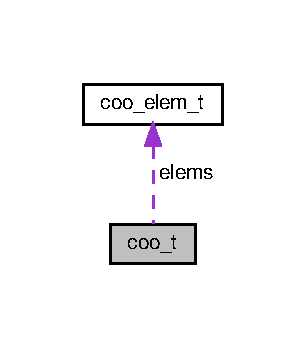
\includegraphics[width=147pt]{structcoo__t__coll__graph}
\end{center}
\end{figure}
\subsection*{Public Attributes}
\begin{DoxyCompactItemize}
\item 
\hyperlink{structcoo__elem__t}{coo\+\_\+elem\+\_\+t} $\ast$ \hyperlink{structcoo__t_a3e74f1e3dadd34e5439f859fab277b54}{elems}
\end{DoxyCompactItemize}


\subsection{Detailed Description}
sparse matrix in coodinate list format 

\subsection{Member Data Documentation}
\mbox{\Hypertarget{structcoo__t_a3e74f1e3dadd34e5439f859fab277b54}\label{structcoo__t_a3e74f1e3dadd34e5439f859fab277b54}} 
\index{coo\+\_\+t@{coo\+\_\+t}!elems@{elems}}
\index{elems@{elems}!coo\+\_\+t@{coo\+\_\+t}}
\subsubsection{\texorpdfstring{elems}{elems}}
{\footnotesize\ttfamily \hyperlink{structcoo__elem__t}{coo\+\_\+elem\+\_\+t}$\ast$ coo\+\_\+t\+::elems}

elements array 

The documentation for this struct was generated from the following file\+:\begin{DoxyCompactItemize}
\item 
/home/tau/public\+\_\+html/lecture/parallel\+\_\+distributed/2018/handson/tau/parallel-\/distributed-\/handson/03spmv/\hyperlink{spmv_8cc}{spmv.\+cc}\end{DoxyCompactItemize}

\hypertarget{structcsr__elem__t}{}\section{csr\+\_\+elem\+\_\+t Struct Reference}
\label{structcsr__elem__t}\index{csr\+\_\+elem\+\_\+t@{csr\+\_\+elem\+\_\+t}}


an element of compressed sparse row  


\subsection*{Public Attributes}
\begin{DoxyCompactItemize}
\item 
\hyperlink{spmv_8cc_a8e93478a00e685bea5e6a3f617bf03a3}{idx\+\_\+t} \hyperlink{structcsr__elem__t_a4525598ab26d6263b2242cc33511ca7f}{j}
\item 
\hyperlink{spmv_8cc_a11d147c64891830c9e79b3315b1b2e21}{real} \hyperlink{structcsr__elem__t_a55e480eefa495ee8b6e359a5f5a94a4f}{a}
\end{DoxyCompactItemize}


\subsection{Detailed Description}
an element of compressed sparse row 

\subsection{Member Data Documentation}
\mbox{\Hypertarget{structcsr__elem__t_a55e480eefa495ee8b6e359a5f5a94a4f}\label{structcsr__elem__t_a55e480eefa495ee8b6e359a5f5a94a4f}} 
\index{csr\+\_\+elem\+\_\+t@{csr\+\_\+elem\+\_\+t}!a@{a}}
\index{a@{a}!csr\+\_\+elem\+\_\+t@{csr\+\_\+elem\+\_\+t}}
\subsubsection{\texorpdfstring{a}{a}}
{\footnotesize\ttfamily \hyperlink{spmv_8cc_a11d147c64891830c9e79b3315b1b2e21}{real} csr\+\_\+elem\+\_\+t\+::a}

element \mbox{\Hypertarget{structcsr__elem__t_a4525598ab26d6263b2242cc33511ca7f}\label{structcsr__elem__t_a4525598ab26d6263b2242cc33511ca7f}} 
\index{csr\+\_\+elem\+\_\+t@{csr\+\_\+elem\+\_\+t}!j@{j}}
\index{j@{j}!csr\+\_\+elem\+\_\+t@{csr\+\_\+elem\+\_\+t}}
\subsubsection{\texorpdfstring{j}{j}}
{\footnotesize\ttfamily \hyperlink{spmv_8cc_a8e93478a00e685bea5e6a3f617bf03a3}{idx\+\_\+t} csr\+\_\+elem\+\_\+t\+::j}

column 

The documentation for this struct was generated from the following file\+:\begin{DoxyCompactItemize}
\item 
/home/tau/public\+\_\+html/lecture/parallel\+\_\+distributed/2018/handson/tau/parallel-\/distributed-\/handson/03spmv/\hyperlink{spmv_8cc}{spmv.\+cc}\end{DoxyCompactItemize}

\hypertarget{structcsr__t}{}\section{csr\+\_\+t Struct Reference}
\label{structcsr__t}\index{csr\+\_\+t@{csr\+\_\+t}}


sparse matrix in compressed row format  




Collaboration diagram for csr\+\_\+t\+:\nopagebreak
\begin{figure}[H]
\begin{center}
\leavevmode
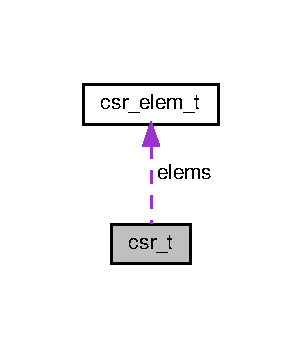
\includegraphics[width=145pt]{structcsr__t__coll__graph}
\end{center}
\end{figure}
\subsection*{Public Attributes}
\begin{DoxyCompactItemize}
\item 
\hyperlink{spmv_8cc_a8e93478a00e685bea5e6a3f617bf03a3}{idx\+\_\+t} $\ast$ \hyperlink{structcsr__t_ac52d7a1ff3a054e2b8c7fcc706e525b6}{row\+\_\+start}
\item 
\hyperlink{structcsr__elem__t}{csr\+\_\+elem\+\_\+t} $\ast$ \hyperlink{structcsr__t_a8fda532ad93e6820aad02feac6bbe04b}{elems}
\end{DoxyCompactItemize}


\subsection{Detailed Description}
sparse matrix in compressed row format 

\subsection{Member Data Documentation}
\mbox{\Hypertarget{structcsr__t_a8fda532ad93e6820aad02feac6bbe04b}\label{structcsr__t_a8fda532ad93e6820aad02feac6bbe04b}} 
\index{csr\+\_\+t@{csr\+\_\+t}!elems@{elems}}
\index{elems@{elems}!csr\+\_\+t@{csr\+\_\+t}}
\subsubsection{\texorpdfstring{elems}{elems}}
{\footnotesize\ttfamily \hyperlink{structcsr__elem__t}{csr\+\_\+elem\+\_\+t}$\ast$ csr\+\_\+t\+::elems}

elements array \mbox{\Hypertarget{structcsr__t_ac52d7a1ff3a054e2b8c7fcc706e525b6}\label{structcsr__t_ac52d7a1ff3a054e2b8c7fcc706e525b6}} 
\index{csr\+\_\+t@{csr\+\_\+t}!row\+\_\+start@{row\+\_\+start}}
\index{row\+\_\+start@{row\+\_\+start}!csr\+\_\+t@{csr\+\_\+t}}
\subsubsection{\texorpdfstring{row\+\_\+start}{row\_start}}
{\footnotesize\ttfamily \hyperlink{spmv_8cc_a8e93478a00e685bea5e6a3f617bf03a3}{idx\+\_\+t}$\ast$ csr\+\_\+t\+::row\+\_\+start}

elems\mbox{[}row\+\_\+start\mbox{[}i\mbox{]}\mbox{]} is the first element of row i 

The documentation for this struct was generated from the following file\+:\begin{DoxyCompactItemize}
\item 
/home/tau/public\+\_\+html/lecture/parallel\+\_\+distributed/2018/handson/tau/parallel-\/distributed-\/handson/03spmv/\hyperlink{spmv_8cc}{spmv.\+cc}\end{DoxyCompactItemize}

\hypertarget{structidx__pair__t}{}\section{idx\+\_\+pair\+\_\+t Struct Reference}
\label{structidx__pair__t}\index{idx\+\_\+pair\+\_\+t@{idx\+\_\+pair\+\_\+t}}


a pair of two indices (i and j)  


\subsection*{Public Attributes}
\begin{DoxyCompactItemize}
\item 
\hyperlink{spmv_8cc_a8e93478a00e685bea5e6a3f617bf03a3}{idx\+\_\+t} \hyperlink{structidx__pair__t_a5fc2a45497e05f6b02ae6dddd4cc5a14}{i}
\item 
\hyperlink{spmv_8cc_a8e93478a00e685bea5e6a3f617bf03a3}{idx\+\_\+t} \hyperlink{structidx__pair__t_afa260eb03684e5ae1c067c13fd33f3e0}{j}
\end{DoxyCompactItemize}


\subsection{Detailed Description}
a pair of two indices (i and j) 

\subsection{Member Data Documentation}
\mbox{\Hypertarget{structidx__pair__t_a5fc2a45497e05f6b02ae6dddd4cc5a14}\label{structidx__pair__t_a5fc2a45497e05f6b02ae6dddd4cc5a14}} 
\index{idx\+\_\+pair\+\_\+t@{idx\+\_\+pair\+\_\+t}!i@{i}}
\index{i@{i}!idx\+\_\+pair\+\_\+t@{idx\+\_\+pair\+\_\+t}}
\subsubsection{\texorpdfstring{i}{i}}
{\footnotesize\ttfamily \hyperlink{spmv_8cc_a8e93478a00e685bea5e6a3f617bf03a3}{idx\+\_\+t} idx\+\_\+pair\+\_\+t\+::i}

row number \mbox{\Hypertarget{structidx__pair__t_afa260eb03684e5ae1c067c13fd33f3e0}\label{structidx__pair__t_afa260eb03684e5ae1c067c13fd33f3e0}} 
\index{idx\+\_\+pair\+\_\+t@{idx\+\_\+pair\+\_\+t}!j@{j}}
\index{j@{j}!idx\+\_\+pair\+\_\+t@{idx\+\_\+pair\+\_\+t}}
\subsubsection{\texorpdfstring{j}{j}}
{\footnotesize\ttfamily \hyperlink{spmv_8cc_a8e93478a00e685bea5e6a3f617bf03a3}{idx\+\_\+t} idx\+\_\+pair\+\_\+t\+::j}

column number 

The documentation for this struct was generated from the following file\+:\begin{DoxyCompactItemize}
\item 
/home/tau/public\+\_\+html/lecture/parallel\+\_\+distributed/2018/handson/tau/parallel-\/distributed-\/handson/03spmv/\hyperlink{spmv_8cc}{spmv.\+cc}\end{DoxyCompactItemize}

\hypertarget{structsparse__format__table__entry__t}{}\section{sparse\+\_\+format\+\_\+table\+\_\+entry\+\_\+t Struct Reference}
\label{structsparse__format__table__entry__t}\index{sparse\+\_\+format\+\_\+table\+\_\+entry\+\_\+t@{sparse\+\_\+format\+\_\+table\+\_\+entry\+\_\+t}}


pair of the index value (sparse\+\_\+format\+\_\+t) and its name  


\subsection*{Public Attributes}
\begin{DoxyCompactItemize}
\item 
\hyperlink{spmv_8cc_a8c0094893526c01b430903b2d9227256}{sparse\+\_\+format\+\_\+t} \hyperlink{structsparse__format__table__entry__t_a1869dde0c0a30270a1f6477c01d530db}{idx}
\item 
const char $\ast$ \hyperlink{structsparse__format__table__entry__t_aff9c31fa7933890b2d4cf0f963df2d89}{name}
\end{DoxyCompactItemize}


\subsection{Detailed Description}
pair of the index value (sparse\+\_\+format\+\_\+t) and its name 

\subsection{Member Data Documentation}
\mbox{\Hypertarget{structsparse__format__table__entry__t_a1869dde0c0a30270a1f6477c01d530db}\label{structsparse__format__table__entry__t_a1869dde0c0a30270a1f6477c01d530db}} 
\index{sparse\+\_\+format\+\_\+table\+\_\+entry\+\_\+t@{sparse\+\_\+format\+\_\+table\+\_\+entry\+\_\+t}!idx@{idx}}
\index{idx@{idx}!sparse\+\_\+format\+\_\+table\+\_\+entry\+\_\+t@{sparse\+\_\+format\+\_\+table\+\_\+entry\+\_\+t}}
\subsubsection{\texorpdfstring{idx}{idx}}
{\footnotesize\ttfamily \hyperlink{spmv_8cc_a8c0094893526c01b430903b2d9227256}{sparse\+\_\+format\+\_\+t} sparse\+\_\+format\+\_\+table\+\_\+entry\+\_\+t\+::idx}

index value \mbox{\Hypertarget{structsparse__format__table__entry__t_aff9c31fa7933890b2d4cf0f963df2d89}\label{structsparse__format__table__entry__t_aff9c31fa7933890b2d4cf0f963df2d89}} 
\index{sparse\+\_\+format\+\_\+table\+\_\+entry\+\_\+t@{sparse\+\_\+format\+\_\+table\+\_\+entry\+\_\+t}!name@{name}}
\index{name@{name}!sparse\+\_\+format\+\_\+table\+\_\+entry\+\_\+t@{sparse\+\_\+format\+\_\+table\+\_\+entry\+\_\+t}}
\subsubsection{\texorpdfstring{name}{name}}
{\footnotesize\ttfamily const char$\ast$ sparse\+\_\+format\+\_\+table\+\_\+entry\+\_\+t\+::name}

name 

The documentation for this struct was generated from the following file\+:\begin{DoxyCompactItemize}
\item 
/home/tau/public\+\_\+html/lecture/parallel\+\_\+distributed/2018/handson/tau/parallel-\/distributed-\/handson/03spmv/\hyperlink{spmv_8cc}{spmv.\+cc}\end{DoxyCompactItemize}

\hypertarget{structsparse__format__table__t}{}\section{sparse\+\_\+format\+\_\+table\+\_\+t Struct Reference}
\label{structsparse__format__table__t}\index{sparse\+\_\+format\+\_\+table\+\_\+t@{sparse\+\_\+format\+\_\+table\+\_\+t}}


table of sparse format and their names  




Collaboration diagram for sparse\+\_\+format\+\_\+table\+\_\+t\+:\nopagebreak
\begin{figure}[H]
\begin{center}
\leavevmode
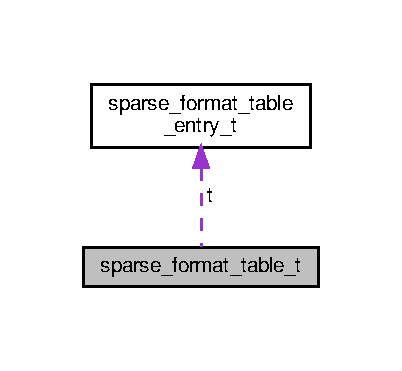
\includegraphics[width=193pt]{structsparse__format__table__t__coll__graph}
\end{center}
\end{figure}
\subsection*{Public Attributes}
\begin{DoxyCompactItemize}
\item 
\hyperlink{structsparse__format__table__entry__t}{sparse\+\_\+format\+\_\+table\+\_\+entry\+\_\+t} \hyperlink{structsparse__format__table__t_aded298a1583f5b097749cf84621c8ef4}{t} \mbox{[}\hyperlink{spmv_8cc_a8c0094893526c01b430903b2d9227256adc326179d0d559f82edc8cd35be11de5}{sparse\+\_\+format\+\_\+invalid}\mbox{]}
\end{DoxyCompactItemize}


\subsection{Detailed Description}
table of sparse format and their names 

\subsection{Member Data Documentation}
\mbox{\Hypertarget{structsparse__format__table__t_aded298a1583f5b097749cf84621c8ef4}\label{structsparse__format__table__t_aded298a1583f5b097749cf84621c8ef4}} 
\index{sparse\+\_\+format\+\_\+table\+\_\+t@{sparse\+\_\+format\+\_\+table\+\_\+t}!t@{t}}
\index{t@{t}!sparse\+\_\+format\+\_\+table\+\_\+t@{sparse\+\_\+format\+\_\+table\+\_\+t}}
\subsubsection{\texorpdfstring{t}{t}}
{\footnotesize\ttfamily \hyperlink{structsparse__format__table__entry__t}{sparse\+\_\+format\+\_\+table\+\_\+entry\+\_\+t} sparse\+\_\+format\+\_\+table\+\_\+t\+::t\mbox{[}\hyperlink{spmv_8cc_a8c0094893526c01b430903b2d9227256adc326179d0d559f82edc8cd35be11de5}{sparse\+\_\+format\+\_\+invalid}\mbox{]}}

array of index value -\/ name pairs 

The documentation for this struct was generated from the following file\+:\begin{DoxyCompactItemize}
\item 
/home/tau/public\+\_\+html/lecture/parallel\+\_\+distributed/2018/handson/tau/parallel-\/distributed-\/handson/03spmv/\hyperlink{spmv_8cc}{spmv.\+cc}\end{DoxyCompactItemize}

\hypertarget{structsparse__matrix__type__table__entry__t}{}\section{sparse\+\_\+matrix\+\_\+type\+\_\+table\+\_\+entry\+\_\+t Struct Reference}
\label{structsparse__matrix__type__table__entry__t}\index{sparse\+\_\+matrix\+\_\+type\+\_\+table\+\_\+entry\+\_\+t@{sparse\+\_\+matrix\+\_\+type\+\_\+table\+\_\+entry\+\_\+t}}


pair of the index value (matrix\+\_\+type\+\_\+t) and its name  


\subsection*{Public Attributes}
\begin{DoxyCompactItemize}
\item 
\hyperlink{spmv_8cc_a43a568fb26bc32aeaad07769cc524c45}{sparse\+\_\+matrix\+\_\+type\+\_\+t} \hyperlink{structsparse__matrix__type__table__entry__t_ae1bbdced2595c2b2e92a75b551631fc4}{idx}
\item 
const char $\ast$ \hyperlink{structsparse__matrix__type__table__entry__t_a7e2dea3171064e4ffece2e2c8a88c9ce}{name}
\end{DoxyCompactItemize}


\subsection{Detailed Description}
pair of the index value (matrix\+\_\+type\+\_\+t) and its name 

\subsection{Member Data Documentation}
\mbox{\Hypertarget{structsparse__matrix__type__table__entry__t_ae1bbdced2595c2b2e92a75b551631fc4}\label{structsparse__matrix__type__table__entry__t_ae1bbdced2595c2b2e92a75b551631fc4}} 
\index{sparse\+\_\+matrix\+\_\+type\+\_\+table\+\_\+entry\+\_\+t@{sparse\+\_\+matrix\+\_\+type\+\_\+table\+\_\+entry\+\_\+t}!idx@{idx}}
\index{idx@{idx}!sparse\+\_\+matrix\+\_\+type\+\_\+table\+\_\+entry\+\_\+t@{sparse\+\_\+matrix\+\_\+type\+\_\+table\+\_\+entry\+\_\+t}}
\subsubsection{\texorpdfstring{idx}{idx}}
{\footnotesize\ttfamily \hyperlink{spmv_8cc_a43a568fb26bc32aeaad07769cc524c45}{sparse\+\_\+matrix\+\_\+type\+\_\+t} sparse\+\_\+matrix\+\_\+type\+\_\+table\+\_\+entry\+\_\+t\+::idx}

index value \mbox{\Hypertarget{structsparse__matrix__type__table__entry__t_a7e2dea3171064e4ffece2e2c8a88c9ce}\label{structsparse__matrix__type__table__entry__t_a7e2dea3171064e4ffece2e2c8a88c9ce}} 
\index{sparse\+\_\+matrix\+\_\+type\+\_\+table\+\_\+entry\+\_\+t@{sparse\+\_\+matrix\+\_\+type\+\_\+table\+\_\+entry\+\_\+t}!name@{name}}
\index{name@{name}!sparse\+\_\+matrix\+\_\+type\+\_\+table\+\_\+entry\+\_\+t@{sparse\+\_\+matrix\+\_\+type\+\_\+table\+\_\+entry\+\_\+t}}
\subsubsection{\texorpdfstring{name}{name}}
{\footnotesize\ttfamily const char$\ast$ sparse\+\_\+matrix\+\_\+type\+\_\+table\+\_\+entry\+\_\+t\+::name}

name 

The documentation for this struct was generated from the following file\+:\begin{DoxyCompactItemize}
\item 
/home/tau/public\+\_\+html/lecture/parallel\+\_\+distributed/2018/handson/tau/parallel-\/distributed-\/handson/03spmv/\hyperlink{spmv_8cc}{spmv.\+cc}\end{DoxyCompactItemize}

\hypertarget{structsparse__matrix__type__table__t}{}\section{sparse\+\_\+matrix\+\_\+type\+\_\+table\+\_\+t Struct Reference}
\label{structsparse__matrix__type__table__t}\index{sparse\+\_\+matrix\+\_\+type\+\_\+table\+\_\+t@{sparse\+\_\+matrix\+\_\+type\+\_\+table\+\_\+t}}


table of sparse matrix types and their names  




Collaboration diagram for sparse\+\_\+matrix\+\_\+type\+\_\+table\+\_\+t\+:\nopagebreak
\begin{figure}[H]
\begin{center}
\leavevmode
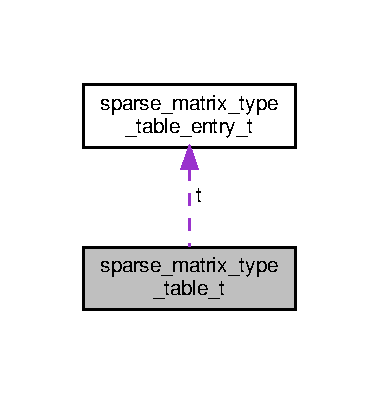
\includegraphics[width=182pt]{structsparse__matrix__type__table__t__coll__graph}
\end{center}
\end{figure}
\subsection*{Public Attributes}
\begin{DoxyCompactItemize}
\item 
\hyperlink{structsparse__matrix__type__table__entry__t}{sparse\+\_\+matrix\+\_\+type\+\_\+table\+\_\+entry\+\_\+t} \hyperlink{structsparse__matrix__type__table__t_a190c83be8b6111d25205a05ed0b23050}{t} \mbox{[}\hyperlink{spmv_8cc_a43a568fb26bc32aeaad07769cc524c45adbd59ebb0cfb220b9035a64fc2ed28dc}{sparse\+\_\+matrix\+\_\+type\+\_\+invalid}\mbox{]}
\end{DoxyCompactItemize}


\subsection{Detailed Description}
table of sparse matrix types and their names 

\subsection{Member Data Documentation}
\mbox{\Hypertarget{structsparse__matrix__type__table__t_a190c83be8b6111d25205a05ed0b23050}\label{structsparse__matrix__type__table__t_a190c83be8b6111d25205a05ed0b23050}} 
\index{sparse\+\_\+matrix\+\_\+type\+\_\+table\+\_\+t@{sparse\+\_\+matrix\+\_\+type\+\_\+table\+\_\+t}!t@{t}}
\index{t@{t}!sparse\+\_\+matrix\+\_\+type\+\_\+table\+\_\+t@{sparse\+\_\+matrix\+\_\+type\+\_\+table\+\_\+t}}
\subsubsection{\texorpdfstring{t}{t}}
{\footnotesize\ttfamily \hyperlink{structsparse__matrix__type__table__entry__t}{sparse\+\_\+matrix\+\_\+type\+\_\+table\+\_\+entry\+\_\+t} sparse\+\_\+matrix\+\_\+type\+\_\+table\+\_\+t\+::t\mbox{[}\hyperlink{spmv_8cc_a43a568fb26bc32aeaad07769cc524c45adbd59ebb0cfb220b9035a64fc2ed28dc}{sparse\+\_\+matrix\+\_\+type\+\_\+invalid}\mbox{]}}

array of index value -\/ name pairs 

The documentation for this struct was generated from the following file\+:\begin{DoxyCompactItemize}
\item 
/home/tau/public\+\_\+html/lecture/parallel\+\_\+distributed/2018/handson/tau/parallel-\/distributed-\/handson/03spmv/\hyperlink{spmv_8cc}{spmv.\+cc}\end{DoxyCompactItemize}

\hypertarget{structsparse__t}{}\section{sparse\+\_\+t Struct Reference}
\label{structsparse__t}\index{sparse\+\_\+t@{sparse\+\_\+t}}


sparse matrix (in any format)  




Collaboration diagram for sparse\+\_\+t\+:\nopagebreak
\begin{figure}[H]
\begin{center}
\leavevmode
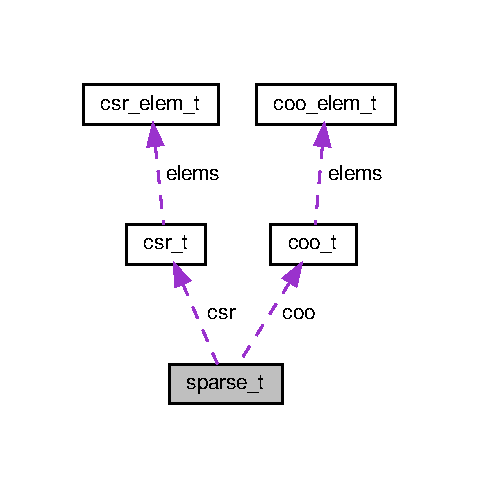
\includegraphics[width=230pt]{structsparse__t__coll__graph}
\end{center}
\end{figure}
\subsection*{Public Attributes}
\begin{DoxyCompactItemize}
\item 
\hyperlink{spmv_8cc_a8c0094893526c01b430903b2d9227256}{sparse\+\_\+format\+\_\+t} \hyperlink{structsparse__t_a1bb9e61c965f9ea814aab21f7ff77a73}{format}
\item 
\hyperlink{spmv_8cc_a8e93478a00e685bea5e6a3f617bf03a3}{idx\+\_\+t} \hyperlink{structsparse__t_a8a08bd7a16c76180afccf05e28f72a93}{M}
\item 
\hyperlink{spmv_8cc_a8e93478a00e685bea5e6a3f617bf03a3}{idx\+\_\+t} \hyperlink{structsparse__t_a418c6deef17a60f31ff11182ea94f85a}{N}
\item 
\hyperlink{spmv_8cc_a8e93478a00e685bea5e6a3f617bf03a3}{idx\+\_\+t} \hyperlink{structsparse__t_ae982d138f3904323b65975769b045a3f}{nnz}
\item 
\mbox{\Hypertarget{structsparse__t_a4d180146ce4a12b0d990cf0e803f7e64}\label{structsparse__t_a4d180146ce4a12b0d990cf0e803f7e64}} 
\begin{tabbing}
xx\=xx\=xx\=xx\=xx\=xx\=xx\=xx\=xx\=\kill
union \{\\
\>\hyperlink{structcoo__t}{coo\_t} \hyperlink{structsparse__t_ad0391f2782f49ea2eb248ed255e9d732}{coo}\\
\>\hyperlink{structcsr__t}{csr\_t} \hyperlink{structsparse__t_a68a71613181b0380d0d4d871236b2521}{csr}\\
\}; \\

\end{tabbing}\end{DoxyCompactItemize}


\subsection{Detailed Description}
sparse matrix (in any format) 

\subsection{Member Data Documentation}
\mbox{\Hypertarget{structsparse__t_ad0391f2782f49ea2eb248ed255e9d732}\label{structsparse__t_ad0391f2782f49ea2eb248ed255e9d732}} 
\index{sparse\+\_\+t@{sparse\+\_\+t}!coo@{coo}}
\index{coo@{coo}!sparse\+\_\+t@{sparse\+\_\+t}}
\subsubsection{\texorpdfstring{coo}{coo}}
{\footnotesize\ttfamily \hyperlink{structcoo__t}{coo\+\_\+t} sparse\+\_\+t\+::coo}

coo or sorted coo \mbox{\Hypertarget{structsparse__t_a68a71613181b0380d0d4d871236b2521}\label{structsparse__t_a68a71613181b0380d0d4d871236b2521}} 
\index{sparse\+\_\+t@{sparse\+\_\+t}!csr@{csr}}
\index{csr@{csr}!sparse\+\_\+t@{sparse\+\_\+t}}
\subsubsection{\texorpdfstring{csr}{csr}}
{\footnotesize\ttfamily \hyperlink{structcsr__t}{csr\+\_\+t} sparse\+\_\+t\+::csr}

csr \mbox{\Hypertarget{structsparse__t_a1bb9e61c965f9ea814aab21f7ff77a73}\label{structsparse__t_a1bb9e61c965f9ea814aab21f7ff77a73}} 
\index{sparse\+\_\+t@{sparse\+\_\+t}!format@{format}}
\index{format@{format}!sparse\+\_\+t@{sparse\+\_\+t}}
\subsubsection{\texorpdfstring{format}{format}}
{\footnotesize\ttfamily \hyperlink{spmv_8cc_a8c0094893526c01b430903b2d9227256}{sparse\+\_\+format\+\_\+t} sparse\+\_\+t\+::format}

format \mbox{\Hypertarget{structsparse__t_a8a08bd7a16c76180afccf05e28f72a93}\label{structsparse__t_a8a08bd7a16c76180afccf05e28f72a93}} 
\index{sparse\+\_\+t@{sparse\+\_\+t}!M@{M}}
\index{M@{M}!sparse\+\_\+t@{sparse\+\_\+t}}
\subsubsection{\texorpdfstring{M}{M}}
{\footnotesize\ttfamily \hyperlink{spmv_8cc_a8e93478a00e685bea5e6a3f617bf03a3}{idx\+\_\+t} sparse\+\_\+t\+::M}

number of rows \mbox{\Hypertarget{structsparse__t_a418c6deef17a60f31ff11182ea94f85a}\label{structsparse__t_a418c6deef17a60f31ff11182ea94f85a}} 
\index{sparse\+\_\+t@{sparse\+\_\+t}!N@{N}}
\index{N@{N}!sparse\+\_\+t@{sparse\+\_\+t}}
\subsubsection{\texorpdfstring{N}{N}}
{\footnotesize\ttfamily \hyperlink{spmv_8cc_a8e93478a00e685bea5e6a3f617bf03a3}{idx\+\_\+t} sparse\+\_\+t\+::N}

number of columns \mbox{\Hypertarget{structsparse__t_ae982d138f3904323b65975769b045a3f}\label{structsparse__t_ae982d138f3904323b65975769b045a3f}} 
\index{sparse\+\_\+t@{sparse\+\_\+t}!nnz@{nnz}}
\index{nnz@{nnz}!sparse\+\_\+t@{sparse\+\_\+t}}
\subsubsection{\texorpdfstring{nnz}{nnz}}
{\footnotesize\ttfamily \hyperlink{spmv_8cc_a8e93478a00e685bea5e6a3f617bf03a3}{idx\+\_\+t} sparse\+\_\+t\+::nnz}

number of non-\/zeros 

The documentation for this struct was generated from the following file\+:\begin{DoxyCompactItemize}
\item 
/home/tau/public\+\_\+html/lecture/parallel\+\_\+distributed/2018/handson/tau/parallel-\/distributed-\/handson/03spmv/\hyperlink{spmv_8cc}{spmv.\+cc}\end{DoxyCompactItemize}

\hypertarget{structspmv__algo__table__entry__t}{}\section{spmv\+\_\+algo\+\_\+table\+\_\+entry\+\_\+t Struct Reference}
\label{structspmv__algo__table__entry__t}\index{spmv\+\_\+algo\+\_\+table\+\_\+entry\+\_\+t@{spmv\+\_\+algo\+\_\+table\+\_\+entry\+\_\+t}}


pair of the index value (spmv\+\_\+algo\+\_\+t) and its name  


\subsection*{Public Attributes}
\begin{DoxyCompactItemize}
\item 
\hyperlink{spmv_8cc_ad2cf0493af54bf76c5be68b4634fcab7}{spmv\+\_\+algo\+\_\+t} \hyperlink{structspmv__algo__table__entry__t_a0ef60703788aaa74667e3bec5f44696d}{idx}
\item 
const char $\ast$ \hyperlink{structspmv__algo__table__entry__t_a0d9006dae288632b43113eeef8aa9f11}{name}
\end{DoxyCompactItemize}


\subsection{Detailed Description}
pair of the index value (spmv\+\_\+algo\+\_\+t) and its name 

\subsection{Member Data Documentation}
\mbox{\Hypertarget{structspmv__algo__table__entry__t_a0ef60703788aaa74667e3bec5f44696d}\label{structspmv__algo__table__entry__t_a0ef60703788aaa74667e3bec5f44696d}} 
\index{spmv\+\_\+algo\+\_\+table\+\_\+entry\+\_\+t@{spmv\+\_\+algo\+\_\+table\+\_\+entry\+\_\+t}!idx@{idx}}
\index{idx@{idx}!spmv\+\_\+algo\+\_\+table\+\_\+entry\+\_\+t@{spmv\+\_\+algo\+\_\+table\+\_\+entry\+\_\+t}}
\subsubsection{\texorpdfstring{idx}{idx}}
{\footnotesize\ttfamily \hyperlink{spmv_8cc_ad2cf0493af54bf76c5be68b4634fcab7}{spmv\+\_\+algo\+\_\+t} spmv\+\_\+algo\+\_\+table\+\_\+entry\+\_\+t\+::idx}

index value \mbox{\Hypertarget{structspmv__algo__table__entry__t_a0d9006dae288632b43113eeef8aa9f11}\label{structspmv__algo__table__entry__t_a0d9006dae288632b43113eeef8aa9f11}} 
\index{spmv\+\_\+algo\+\_\+table\+\_\+entry\+\_\+t@{spmv\+\_\+algo\+\_\+table\+\_\+entry\+\_\+t}!name@{name}}
\index{name@{name}!spmv\+\_\+algo\+\_\+table\+\_\+entry\+\_\+t@{spmv\+\_\+algo\+\_\+table\+\_\+entry\+\_\+t}}
\subsubsection{\texorpdfstring{name}{name}}
{\footnotesize\ttfamily const char$\ast$ spmv\+\_\+algo\+\_\+table\+\_\+entry\+\_\+t\+::name}

name 

The documentation for this struct was generated from the following file\+:\begin{DoxyCompactItemize}
\item 
/home/tau/public\+\_\+html/lecture/parallel\+\_\+distributed/2018/handson/tau/parallel-\/distributed-\/handson/03spmv/\hyperlink{spmv_8cc}{spmv.\+cc}\end{DoxyCompactItemize}

\hypertarget{structspmv__algo__table__t}{}\section{spmv\+\_\+algo\+\_\+table\+\_\+t Struct Reference}
\label{structspmv__algo__table__t}\index{spmv\+\_\+algo\+\_\+table\+\_\+t@{spmv\+\_\+algo\+\_\+table\+\_\+t}}


table of spmv algorithms and their names  




Collaboration diagram for spmv\+\_\+algo\+\_\+table\+\_\+t\+:\nopagebreak
\begin{figure}[H]
\begin{center}
\leavevmode
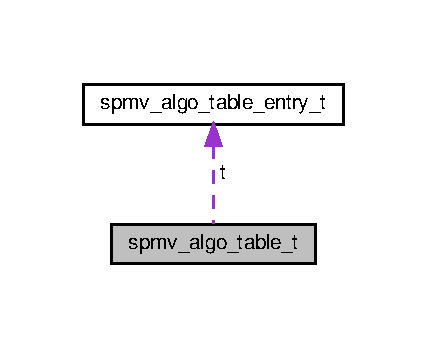
\includegraphics[width=205pt]{structspmv__algo__table__t__coll__graph}
\end{center}
\end{figure}
\subsection*{Public Attributes}
\begin{DoxyCompactItemize}
\item 
\hyperlink{structspmv__algo__table__entry__t}{spmv\+\_\+algo\+\_\+table\+\_\+entry\+\_\+t} \hyperlink{structspmv__algo__table__t_a8cc8ce6a17f236df757787d28ae93315}{t} \mbox{[}\hyperlink{spmv_8cc_ad2cf0493af54bf76c5be68b4634fcab7add2a1e0329d677ee5f5fcc7ee8077dd0}{spmv\+\_\+algo\+\_\+invalid}\mbox{]}
\end{DoxyCompactItemize}


\subsection{Detailed Description}
table of spmv algorithms and their names 

\subsection{Member Data Documentation}
\mbox{\Hypertarget{structspmv__algo__table__t_a8cc8ce6a17f236df757787d28ae93315}\label{structspmv__algo__table__t_a8cc8ce6a17f236df757787d28ae93315}} 
\index{spmv\+\_\+algo\+\_\+table\+\_\+t@{spmv\+\_\+algo\+\_\+table\+\_\+t}!t@{t}}
\index{t@{t}!spmv\+\_\+algo\+\_\+table\+\_\+t@{spmv\+\_\+algo\+\_\+table\+\_\+t}}
\subsubsection{\texorpdfstring{t}{t}}
{\footnotesize\ttfamily \hyperlink{structspmv__algo__table__entry__t}{spmv\+\_\+algo\+\_\+table\+\_\+entry\+\_\+t} spmv\+\_\+algo\+\_\+table\+\_\+t\+::t\mbox{[}\hyperlink{spmv_8cc_ad2cf0493af54bf76c5be68b4634fcab7add2a1e0329d677ee5f5fcc7ee8077dd0}{spmv\+\_\+algo\+\_\+invalid}\mbox{]}}

array of index value -\/ name pairs 

The documentation for this struct was generated from the following file\+:\begin{DoxyCompactItemize}
\item 
/home/tau/public\+\_\+html/lecture/parallel\+\_\+distributed/2018/handson/tau/parallel-\/distributed-\/handson/03spmv/\hyperlink{spmv_8cc}{spmv.\+cc}\end{DoxyCompactItemize}

\hypertarget{structvec__t}{}\section{vec\+\_\+t Struct Reference}
\label{structvec__t}\index{vec\+\_\+t@{vec\+\_\+t}}


vector  


\subsection*{Public Attributes}
\begin{DoxyCompactItemize}
\item 
\hyperlink{spmv_8cc_a8e93478a00e685bea5e6a3f617bf03a3}{idx\+\_\+t} \hyperlink{structvec__t_a06879ff4054298fbc680b02e3e18da7a}{n}
\item 
\hyperlink{spmv_8cc_a11d147c64891830c9e79b3315b1b2e21}{real} $\ast$ \hyperlink{structvec__t_a7d62f0b683ab0558903c5227d670ac1a}{elems}
\end{DoxyCompactItemize}


\subsection{Detailed Description}
vector 

\subsection{Member Data Documentation}
\mbox{\Hypertarget{structvec__t_a7d62f0b683ab0558903c5227d670ac1a}\label{structvec__t_a7d62f0b683ab0558903c5227d670ac1a}} 
\index{vec\+\_\+t@{vec\+\_\+t}!elems@{elems}}
\index{elems@{elems}!vec\+\_\+t@{vec\+\_\+t}}
\subsubsection{\texorpdfstring{elems}{elems}}
{\footnotesize\ttfamily \hyperlink{spmv_8cc_a11d147c64891830c9e79b3315b1b2e21}{real}$\ast$ vec\+\_\+t\+::elems}

array of elements \mbox{\Hypertarget{structvec__t_a06879ff4054298fbc680b02e3e18da7a}\label{structvec__t_a06879ff4054298fbc680b02e3e18da7a}} 
\index{vec\+\_\+t@{vec\+\_\+t}!n@{n}}
\index{n@{n}!vec\+\_\+t@{vec\+\_\+t}}
\subsubsection{\texorpdfstring{n}{n}}
{\footnotesize\ttfamily \hyperlink{spmv_8cc_a8e93478a00e685bea5e6a3f617bf03a3}{idx\+\_\+t} vec\+\_\+t\+::n}

number of elements 

The documentation for this struct was generated from the following file\+:\begin{DoxyCompactItemize}
\item 
/home/tau/public\+\_\+html/lecture/parallel\+\_\+distributed/2018/handson/tau/parallel-\/distributed-\/handson/03spmv/\hyperlink{spmv_8cc}{spmv.\+cc}\end{DoxyCompactItemize}

\chapter{File Documentation}
\hypertarget{coo__to__dev_8cc}{}\section{/home/tau/public\+\_\+html/lecture/parallel\+\_\+distributed/2018/handson/tau/parallel-\/distributed-\/handson/03spmv/include/coo\+\_\+to\+\_\+dev.cc File Reference}
\label{coo__to__dev_8cc}\index{/home/tau/public\+\_\+html/lecture/parallel\+\_\+distributed/2018/handson/tau/parallel-\/distributed-\/handson/03spmv/include/coo\+\_\+to\+\_\+dev.\+cc@{/home/tau/public\+\_\+html/lecture/parallel\+\_\+distributed/2018/handson/tau/parallel-\/distributed-\/handson/03spmv/include/coo\+\_\+to\+\_\+dev.\+cc}}


make a deivce copy of a sparse matrix in coo format  


\subsection*{Functions}
\begin{DoxyCompactItemize}
\item 
static int \hyperlink{coo__to__dev_8cc_ab0c33415be097ee3c3d142d348d656c3}{coo\+\_\+to\+\_\+dev} (\hyperlink{structsparse__t}{sparse\+\_\+t} \&A)
\begin{DoxyCompactList}\small\item\em make a deivce copy of a sparse matrix in coo format. \end{DoxyCompactList}\end{DoxyCompactItemize}


\subsection{Detailed Description}
make a deivce copy of a sparse matrix in coo format 



\subsection{Function Documentation}
\mbox{\Hypertarget{coo__to__dev_8cc_ab0c33415be097ee3c3d142d348d656c3}\label{coo__to__dev_8cc_ab0c33415be097ee3c3d142d348d656c3}} 
\index{coo\+\_\+to\+\_\+dev.\+cc@{coo\+\_\+to\+\_\+dev.\+cc}!coo\+\_\+to\+\_\+dev@{coo\+\_\+to\+\_\+dev}}
\index{coo\+\_\+to\+\_\+dev@{coo\+\_\+to\+\_\+dev}!coo\+\_\+to\+\_\+dev.\+cc@{coo\+\_\+to\+\_\+dev.\+cc}}
\subsubsection{\texorpdfstring{coo\+\_\+to\+\_\+dev()}{coo\_to\_dev()}}
{\footnotesize\ttfamily static int coo\+\_\+to\+\_\+dev (\begin{DoxyParamCaption}\item[{\hyperlink{structsparse__t}{sparse\+\_\+t} \&}]{A }\end{DoxyParamCaption})\hspace{0.3cm}{\ttfamily [static]}}



make a deivce copy of a sparse matrix in coo format. 


\begin{DoxyParams}{Parameters}
{\em (\+A)} & the reference to a matrix whose elems\+\_\+dev has not been set (i.\+e., = N\+U\+LL) \\
\hline
\end{DoxyParams}
\begin{DoxyReturn}{Returns}
1 if succeed. 0 if failed.
\end{DoxyReturn}
this function allocates memory on the device and transfers A\textquotesingle{}s non-\/zero elements in the allocated memory. it also should set A\textquotesingle{}s elems\+\_\+dev to the address of the allocated memory, so that if you pass A as an argument of a kernel launch, the device code can obtain all necessary information of A from the parameter. \begin{DoxySeeAlso}{See also}
sparse\+\_\+to\+\_\+dev 
\end{DoxySeeAlso}

\hypertarget{csr__to__dev_8cc}{}\section{/home/tau/public\+\_\+html/lecture/parallel\+\_\+distributed/2018/handson/tau/parallel-\/distributed-\/handson/03spmv/include/csr\+\_\+to\+\_\+dev.cc File Reference}
\label{csr__to__dev_8cc}\index{/home/tau/public\+\_\+html/lecture/parallel\+\_\+distributed/2018/handson/tau/parallel-\/distributed-\/handson/03spmv/include/csr\+\_\+to\+\_\+dev.\+cc@{/home/tau/public\+\_\+html/lecture/parallel\+\_\+distributed/2018/handson/tau/parallel-\/distributed-\/handson/03spmv/include/csr\+\_\+to\+\_\+dev.\+cc}}


make a deivce copy of a sparse matrix in csr format  


\subsection*{Functions}
\begin{DoxyCompactItemize}
\item 
static int \hyperlink{csr__to__dev_8cc_a6fae0ec490809d89e56593b0aba9da82}{csr\+\_\+to\+\_\+dev} (\hyperlink{structsparse__t}{sparse\+\_\+t} \&A)
\begin{DoxyCompactList}\small\item\em make a deivce copy of a sparse matrix in csr format. \end{DoxyCompactList}\end{DoxyCompactItemize}


\subsection{Detailed Description}
make a deivce copy of a sparse matrix in csr format 



\subsection{Function Documentation}
\mbox{\Hypertarget{csr__to__dev_8cc_a6fae0ec490809d89e56593b0aba9da82}\label{csr__to__dev_8cc_a6fae0ec490809d89e56593b0aba9da82}} 
\index{csr\+\_\+to\+\_\+dev.\+cc@{csr\+\_\+to\+\_\+dev.\+cc}!csr\+\_\+to\+\_\+dev@{csr\+\_\+to\+\_\+dev}}
\index{csr\+\_\+to\+\_\+dev@{csr\+\_\+to\+\_\+dev}!csr\+\_\+to\+\_\+dev.\+cc@{csr\+\_\+to\+\_\+dev.\+cc}}
\subsubsection{\texorpdfstring{csr\+\_\+to\+\_\+dev()}{csr\_to\_dev()}}
{\footnotesize\ttfamily static int csr\+\_\+to\+\_\+dev (\begin{DoxyParamCaption}\item[{\hyperlink{structsparse__t}{sparse\+\_\+t} \&}]{A }\end{DoxyParamCaption})\hspace{0.3cm}{\ttfamily [static]}}



make a deivce copy of a sparse matrix in csr format. 


\begin{DoxyParams}{Parameters}
{\em (\+A)} & the reference to a matrix whose elems\+\_\+dev has not been set (i.\+e., = N\+U\+LL) \\
\hline
\end{DoxyParams}
\begin{DoxyReturn}{Returns}
1 if succeed. 0 if failed.
\end{DoxyReturn}
this function allocates memory blocks on the device and transfers A\textquotesingle{}s row\+\_\+start array and non-\/zero elements in the allocated blocks. it also should set A\textquotesingle{}s elems\+\_\+dev and row\+\_\+start\+\_\+dev to the addresses of the allocated blocks, so that if you pass A as an argument of a kernel launch, the device code can obtain all necessary information of A from the parameter. \begin{DoxySeeAlso}{See also}
sparse\+\_\+to\+\_\+dev 
\end{DoxySeeAlso}

\hypertarget{cuda__util_8h}{}\section{/home/tau/public\+\_\+html/lecture/parallel\+\_\+distributed/2018/handson/tau/parallel-\/distributed-\/handson/03spmv/include/cuda\+\_\+util.h File Reference}
\label{cuda__util_8h}\index{/home/tau/public\+\_\+html/lecture/parallel\+\_\+distributed/2018/handson/tau/parallel-\/distributed-\/handson/03spmv/include/cuda\+\_\+util.\+h@{/home/tau/public\+\_\+html/lecture/parallel\+\_\+distributed/2018/handson/tau/parallel-\/distributed-\/handson/03spmv/include/cuda\+\_\+util.\+h}}


small utility functions for cuda  


\subsection*{Macros}
\begin{DoxyCompactItemize}
\item 
\#define \hyperlink{cuda__util_8h_ae08da20e750e9eabdf37c5cdf87a6e73}{check\+\_\+api\+\_\+error}(e)~\hyperlink{cuda__util_8h_afe8e81182b6d9bdc912e4477ea7f6221}{check\+\_\+api\+\_\+error\+\_\+}(e, \#e, \+\_\+\+\_\+\+F\+I\+L\+E\+\_\+\+\_\+, \+\_\+\+\_\+\+L\+I\+N\+E\+\_\+\+\_\+)
\begin{DoxyCompactList}\small\item\em check if a C\+U\+DA A\+PI invocation succeeded and show the error msg if any \end{DoxyCompactList}\item 
\#define \hyperlink{cuda__util_8h_ae8a9e1ffcd7af83a818bc9a6ec7bed78}{check\+\_\+launch\+\_\+error}(exp)~do \{ exp; \hyperlink{cuda__util_8h_a522422f538aba091ae7b9ec113871075}{check\+\_\+launch\+\_\+error\+\_\+}(\#exp, \+\_\+\+\_\+\+F\+I\+L\+E\+\_\+\+\_\+, \+\_\+\+\_\+\+L\+I\+N\+E\+\_\+\+\_\+); \} while (0)
\begin{DoxyCompactList}\small\item\em check kernel launch error \end{DoxyCompactList}\end{DoxyCompactItemize}
\subsection*{Functions}
\begin{DoxyCompactItemize}
\item 
static void \hyperlink{cuda__util_8h_afe8e81182b6d9bdc912e4477ea7f6221}{check\+\_\+api\+\_\+error\+\_\+} (cuda\+Error\+\_\+t e, const char $\ast$msg, const char $\ast$file, int line)
\begin{DoxyCompactList}\small\item\em do not use this function directly. use check\+\_\+api\+\_\+error macro \end{DoxyCompactList}\item 
static void \hyperlink{cuda__util_8h_a522422f538aba091ae7b9ec113871075}{check\+\_\+launch\+\_\+error\+\_\+} (const char $\ast$msg, const char $\ast$file, int line)
\begin{DoxyCompactList}\small\item\em do not use this function directly. use check\+\_\+launch\+\_\+error macro \end{DoxyCompactList}\item 
\mbox{\Hypertarget{cuda__util_8h_a42ba739c08e201d58f7a031d899a0e7f}\label{cuda__util_8h_a42ba739c08e201d58f7a031d899a0e7f}} 
\+\_\+\+\_\+device\+\_\+\+\_\+ uint \hyperlink{cuda__util_8h_a42ba739c08e201d58f7a031d899a0e7f}{get\+\_\+smid} (void)
\begin{DoxyCompactList}\small\item\em get SM executing the caller \end{DoxyCompactList}\item 
\mbox{\Hypertarget{cuda__util_8h_a859de24e23ee0450818ab96ea6a4798a}\label{cuda__util_8h_a859de24e23ee0450818ab96ea6a4798a}} 
static int \hyperlink{cuda__util_8h_a859de24e23ee0450818ab96ea6a4798a}{get\+\_\+freq} ()
\begin{DoxyCompactList}\small\item\em get device frequency \end{DoxyCompactList}\item 
\mbox{\Hypertarget{cuda__util_8h_afefb7dee05552efd8d1e91a09c90dc79}\label{cuda__util_8h_afefb7dee05552efd8d1e91a09c90dc79}} 
static void $\ast$ \hyperlink{cuda__util_8h_afefb7dee05552efd8d1e91a09c90dc79}{dev\+\_\+malloc} (size\+\_\+t sz)
\begin{DoxyCompactList}\small\item\em wrap cuda\+Malloc. cuda\+Malloc + error check + more ordinary malloc-\/like interface (return pointer) \end{DoxyCompactList}\item 
\mbox{\Hypertarget{cuda__util_8h_ade14b7c582717d436e547ed0fcf8e4fe}\label{cuda__util_8h_ade14b7c582717d436e547ed0fcf8e4fe}} 
static void \hyperlink{cuda__util_8h_ade14b7c582717d436e547ed0fcf8e4fe}{dev\+\_\+free} (void $\ast$a)
\begin{DoxyCompactList}\small\item\em wrap cuda\+Free \end{DoxyCompactList}\item 
\mbox{\Hypertarget{cuda__util_8h_a0737678a7fc54cb0347e3c4178ad5dfa}\label{cuda__util_8h_a0737678a7fc54cb0347e3c4178ad5dfa}} 
void \hyperlink{cuda__util_8h_a0737678a7fc54cb0347e3c4178ad5dfa}{to\+\_\+host} (void $\ast$dst, void $\ast$src, size\+\_\+t sz)
\begin{DoxyCompactList}\small\item\em wrap cuda\+Memcpy to copy from device to host (and check an error if any) \end{DoxyCompactList}\item 
\mbox{\Hypertarget{cuda__util_8h_a7b851642eafb77c5d1945bcf81916d7c}\label{cuda__util_8h_a7b851642eafb77c5d1945bcf81916d7c}} 
static void \hyperlink{cuda__util_8h_a7b851642eafb77c5d1945bcf81916d7c}{to\+\_\+dev} (void $\ast$dst, void $\ast$src, size\+\_\+t sz)
\begin{DoxyCompactList}\small\item\em wrap cuda\+Memcpy to copy from host to device (and check an error if any) \end{DoxyCompactList}\item 
\mbox{\Hypertarget{cuda__util_8h_a30655f0f077528b999634c85513af4b0}\label{cuda__util_8h_a30655f0f077528b999634c85513af4b0}} 
\+\_\+\+\_\+device\+\_\+\+\_\+ int \hyperlink{cuda__util_8h_a30655f0f077528b999634c85513af4b0}{get\+\_\+thread\+\_\+id\+\_\+x} ()
\begin{DoxyCompactList}\small\item\em thread ID along x-\/dimension \end{DoxyCompactList}\item 
\mbox{\Hypertarget{cuda__util_8h_a6ea184310bf6fc2e1313127215aab5b0}\label{cuda__util_8h_a6ea184310bf6fc2e1313127215aab5b0}} 
\+\_\+\+\_\+device\+\_\+\+\_\+ int \hyperlink{cuda__util_8h_a6ea184310bf6fc2e1313127215aab5b0}{get\+\_\+thread\+\_\+id\+\_\+y} ()
\begin{DoxyCompactList}\small\item\em thread ID along y-\/dimension \end{DoxyCompactList}\item 
\mbox{\Hypertarget{cuda__util_8h_afff8c5c6d0e85b4a264786a4170ad777}\label{cuda__util_8h_afff8c5c6d0e85b4a264786a4170ad777}} 
\+\_\+\+\_\+device\+\_\+\+\_\+ int \hyperlink{cuda__util_8h_afff8c5c6d0e85b4a264786a4170ad777}{get\+\_\+thread\+\_\+id\+\_\+z} ()
\begin{DoxyCompactList}\small\item\em thread ID along z-\/dimension \end{DoxyCompactList}\item 
\mbox{\Hypertarget{cuda__util_8h_ae13980c33ac8f950ed35d613415034c0}\label{cuda__util_8h_ae13980c33ac8f950ed35d613415034c0}} 
\+\_\+\+\_\+device\+\_\+\+\_\+ int \hyperlink{cuda__util_8h_ae13980c33ac8f950ed35d613415034c0}{get\+\_\+nthreads\+\_\+x} ()
\begin{DoxyCompactList}\small\item\em number of threads along x-\/dimension \end{DoxyCompactList}\item 
\mbox{\Hypertarget{cuda__util_8h_a79fd9ff68db3a81b8b0feb446e4e9b99}\label{cuda__util_8h_a79fd9ff68db3a81b8b0feb446e4e9b99}} 
\+\_\+\+\_\+device\+\_\+\+\_\+ int \hyperlink{cuda__util_8h_a79fd9ff68db3a81b8b0feb446e4e9b99}{get\+\_\+nthreads\+\_\+y} ()
\begin{DoxyCompactList}\small\item\em number of threads along y-\/dimension \end{DoxyCompactList}\item 
\mbox{\Hypertarget{cuda__util_8h_a59cd23ec9bc1ab07e3eaac1ad3e109b4}\label{cuda__util_8h_a59cd23ec9bc1ab07e3eaac1ad3e109b4}} 
\+\_\+\+\_\+device\+\_\+\+\_\+ int \hyperlink{cuda__util_8h_a59cd23ec9bc1ab07e3eaac1ad3e109b4}{get\+\_\+nthreads\+\_\+z} ()
\begin{DoxyCompactList}\small\item\em number of threads along z-\/dimension \end{DoxyCompactList}\item 
\mbox{\Hypertarget{cuda__util_8h_ace44c6e6794929ce9e48e1122c7a3a12}\label{cuda__util_8h_ace44c6e6794929ce9e48e1122c7a3a12}} 
\+\_\+\+\_\+device\+\_\+\+\_\+ int \hyperlink{cuda__util_8h_ace44c6e6794929ce9e48e1122c7a3a12}{get\+\_\+thread\+\_\+id} ()
\begin{DoxyCompactList}\small\item\em global (x,y,z combined into an integer) thread ID \end{DoxyCompactList}\item 
\mbox{\Hypertarget{cuda__util_8h_a74d008c0d996e10f203bdd1fdee76511}\label{cuda__util_8h_a74d008c0d996e10f203bdd1fdee76511}} 
\+\_\+\+\_\+device\+\_\+\+\_\+ int \hyperlink{cuda__util_8h_a74d008c0d996e10f203bdd1fdee76511}{get\+\_\+nthreads} ()
\begin{DoxyCompactList}\small\item\em total number of threads \end{DoxyCompactList}\end{DoxyCompactItemize}


\subsection{Detailed Description}
small utility functions for cuda 

\begin{DoxyAuthor}{Author}
Kenjiro Taura 
\end{DoxyAuthor}
\begin{DoxyDate}{Date}
Oct. 14, 2018 
\end{DoxyDate}


\subsection{Macro Definition Documentation}
\mbox{\Hypertarget{cuda__util_8h_ae08da20e750e9eabdf37c5cdf87a6e73}\label{cuda__util_8h_ae08da20e750e9eabdf37c5cdf87a6e73}} 
\index{cuda\+\_\+util.\+h@{cuda\+\_\+util.\+h}!check\+\_\+api\+\_\+error@{check\+\_\+api\+\_\+error}}
\index{check\+\_\+api\+\_\+error@{check\+\_\+api\+\_\+error}!cuda\+\_\+util.\+h@{cuda\+\_\+util.\+h}}
\subsubsection{\texorpdfstring{check\+\_\+api\+\_\+error}{check\_api\_error}}
{\footnotesize\ttfamily \#define check\+\_\+api\+\_\+error(\begin{DoxyParamCaption}\item[{}]{e }\end{DoxyParamCaption})~\hyperlink{cuda__util_8h_afe8e81182b6d9bdc912e4477ea7f6221}{check\+\_\+api\+\_\+error\+\_\+}(e, \#e, \+\_\+\+\_\+\+F\+I\+L\+E\+\_\+\+\_\+, \+\_\+\+\_\+\+L\+I\+N\+E\+\_\+\+\_\+)}



check if a C\+U\+DA A\+PI invocation succeeded and show the error msg if any 

usage\+: \hyperlink{cuda__util_8h_ae08da20e750e9eabdf37c5cdf87a6e73}{check\+\_\+api\+\_\+error(cuda\+\_\+api\+\_\+call())}. for example, \hyperlink{cuda__util_8h_ae08da20e750e9eabdf37c5cdf87a6e73}{check\+\_\+api\+\_\+error(cuda\+Malloc(\&p, size))}; \mbox{\Hypertarget{cuda__util_8h_ae8a9e1ffcd7af83a818bc9a6ec7bed78}\label{cuda__util_8h_ae8a9e1ffcd7af83a818bc9a6ec7bed78}} 
\index{cuda\+\_\+util.\+h@{cuda\+\_\+util.\+h}!check\+\_\+launch\+\_\+error@{check\+\_\+launch\+\_\+error}}
\index{check\+\_\+launch\+\_\+error@{check\+\_\+launch\+\_\+error}!cuda\+\_\+util.\+h@{cuda\+\_\+util.\+h}}
\subsubsection{\texorpdfstring{check\+\_\+launch\+\_\+error}{check\_launch\_error}}
{\footnotesize\ttfamily \#define check\+\_\+launch\+\_\+error(\begin{DoxyParamCaption}\item[{}]{exp }\end{DoxyParamCaption})~do \{ exp; \hyperlink{cuda__util_8h_a522422f538aba091ae7b9ec113871075}{check\+\_\+launch\+\_\+error\+\_\+}(\#exp, \+\_\+\+\_\+\+F\+I\+L\+E\+\_\+\+\_\+, \+\_\+\+\_\+\+L\+I\+N\+E\+\_\+\+\_\+); \} while (0)}



check kernel launch error 

usage\+: check\+\_\+launch\+\_\+error((kernel-\/launch-\/expression)). for example, check\+\_\+launch\+\_\+error((your\+\_\+gpu\+\_\+kernel$<$$<$$<$n\+\_\+blocks,block\+\_\+sz$>$$>$$>$(a,b,c))). note that you need to put parens around the expression. 

\subsection{Function Documentation}
\mbox{\Hypertarget{cuda__util_8h_afe8e81182b6d9bdc912e4477ea7f6221}\label{cuda__util_8h_afe8e81182b6d9bdc912e4477ea7f6221}} 
\index{cuda\+\_\+util.\+h@{cuda\+\_\+util.\+h}!check\+\_\+api\+\_\+error\+\_\+@{check\+\_\+api\+\_\+error\+\_\+}}
\index{check\+\_\+api\+\_\+error\+\_\+@{check\+\_\+api\+\_\+error\+\_\+}!cuda\+\_\+util.\+h@{cuda\+\_\+util.\+h}}
\subsubsection{\texorpdfstring{check\+\_\+api\+\_\+error\+\_\+()}{check\_api\_error\_()}}
{\footnotesize\ttfamily static void check\+\_\+api\+\_\+error\+\_\+ (\begin{DoxyParamCaption}\item[{cuda\+Error\+\_\+t}]{e,  }\item[{const char $\ast$}]{msg,  }\item[{const char $\ast$}]{file,  }\item[{int}]{line }\end{DoxyParamCaption})\hspace{0.3cm}{\ttfamily [static]}}



do not use this function directly. use check\+\_\+api\+\_\+error macro 

\begin{DoxySeeAlso}{See also}
\hyperlink{cuda__util_8h_ae08da20e750e9eabdf37c5cdf87a6e73}{check\+\_\+api\+\_\+error} 
\end{DoxySeeAlso}
\mbox{\Hypertarget{cuda__util_8h_a522422f538aba091ae7b9ec113871075}\label{cuda__util_8h_a522422f538aba091ae7b9ec113871075}} 
\index{cuda\+\_\+util.\+h@{cuda\+\_\+util.\+h}!check\+\_\+launch\+\_\+error\+\_\+@{check\+\_\+launch\+\_\+error\+\_\+}}
\index{check\+\_\+launch\+\_\+error\+\_\+@{check\+\_\+launch\+\_\+error\+\_\+}!cuda\+\_\+util.\+h@{cuda\+\_\+util.\+h}}
\subsubsection{\texorpdfstring{check\+\_\+launch\+\_\+error\+\_\+()}{check\_launch\_error\_()}}
{\footnotesize\ttfamily static void check\+\_\+launch\+\_\+error\+\_\+ (\begin{DoxyParamCaption}\item[{const char $\ast$}]{msg,  }\item[{const char $\ast$}]{file,  }\item[{int}]{line }\end{DoxyParamCaption})\hspace{0.3cm}{\ttfamily [static]}}



do not use this function directly. use check\+\_\+launch\+\_\+error macro 

\begin{DoxySeeAlso}{See also}
\hyperlink{cuda__util_8h_ae8a9e1ffcd7af83a818bc9a6ec7bed78}{check\+\_\+launch\+\_\+error} 
\end{DoxySeeAlso}

\hypertarget{scalar__vec__cuda_8cc}{}\section{/home/tau/public\+\_\+html/lecture/parallel\+\_\+distributed/2018/handson/tau/parallel-\/distributed-\/handson/03spmv/include/scalar\+\_\+vec\+\_\+cuda.cc File Reference}
\label{scalar__vec__cuda_8cc}\index{/home/tau/public\+\_\+html/lecture/parallel\+\_\+distributed/2018/handson/tau/parallel-\/distributed-\/handson/03spmv/include/scalar\+\_\+vec\+\_\+cuda.\+cc@{/home/tau/public\+\_\+html/lecture/parallel\+\_\+distributed/2018/handson/tau/parallel-\/distributed-\/handson/03spmv/include/scalar\+\_\+vec\+\_\+cuda.\+cc}}


scalar x vector multiply with cuda  


\subsection*{Functions}
\begin{DoxyCompactItemize}
\item 
\+\_\+\+\_\+global\+\_\+\+\_\+ void \hyperlink{scalar__vec__cuda_8cc_a34eb85affb310250923e68a6c7ae361f}{scalar\+\_\+vec\+\_\+dev} (\hyperlink{spmv_8cc_a11d147c64891830c9e79b3315b1b2e21}{real} k, \hyperlink{structvec__t}{vec\+\_\+t} v)
\begin{DoxyCompactList}\small\item\em the device procedure for k x v in parallel with cuda \end{DoxyCompactList}\item 
static int \hyperlink{scalar__vec__cuda_8cc_a79a39db6a0400b471d1a5922696cf476}{scalar\+\_\+vec\+\_\+cuda} (\hyperlink{spmv_8cc_a11d147c64891830c9e79b3315b1b2e21}{real} k, \hyperlink{structvec__t}{vec\+\_\+t} v)
\begin{DoxyCompactList}\small\item\em k x v in parallel with cuda \end{DoxyCompactList}\end{DoxyCompactItemize}


\subsection{Detailed Description}
scalar x vector multiply with cuda 



\subsection{Function Documentation}
\mbox{\Hypertarget{scalar__vec__cuda_8cc_a79a39db6a0400b471d1a5922696cf476}\label{scalar__vec__cuda_8cc_a79a39db6a0400b471d1a5922696cf476}} 
\index{scalar\+\_\+vec\+\_\+cuda.\+cc@{scalar\+\_\+vec\+\_\+cuda.\+cc}!scalar\+\_\+vec\+\_\+cuda@{scalar\+\_\+vec\+\_\+cuda}}
\index{scalar\+\_\+vec\+\_\+cuda@{scalar\+\_\+vec\+\_\+cuda}!scalar\+\_\+vec\+\_\+cuda.\+cc@{scalar\+\_\+vec\+\_\+cuda.\+cc}}
\subsubsection{\texorpdfstring{scalar\+\_\+vec\+\_\+cuda()}{scalar\_vec\_cuda()}}
{\footnotesize\ttfamily static int scalar\+\_\+vec\+\_\+cuda (\begin{DoxyParamCaption}\item[{\hyperlink{spmv_8cc_a11d147c64891830c9e79b3315b1b2e21}{real}}]{k,  }\item[{\hyperlink{structvec__t}{vec\+\_\+t}}]{v }\end{DoxyParamCaption})\hspace{0.3cm}{\ttfamily [static]}}



k x v in parallel with cuda 


\begin{DoxyParams}{Parameters}
{\em (k)} & a scalar \\
\hline
{\em (v)} & a vector\\
\hline
\end{DoxyParams}
multiply each element of v by k \mbox{\Hypertarget{scalar__vec__cuda_8cc_a34eb85affb310250923e68a6c7ae361f}\label{scalar__vec__cuda_8cc_a34eb85affb310250923e68a6c7ae361f}} 
\index{scalar\+\_\+vec\+\_\+cuda.\+cc@{scalar\+\_\+vec\+\_\+cuda.\+cc}!scalar\+\_\+vec\+\_\+dev@{scalar\+\_\+vec\+\_\+dev}}
\index{scalar\+\_\+vec\+\_\+dev@{scalar\+\_\+vec\+\_\+dev}!scalar\+\_\+vec\+\_\+cuda.\+cc@{scalar\+\_\+vec\+\_\+cuda.\+cc}}
\subsubsection{\texorpdfstring{scalar\+\_\+vec\+\_\+dev()}{scalar\_vec\_dev()}}
{\footnotesize\ttfamily \+\_\+\+\_\+global\+\_\+\+\_\+ void scalar\+\_\+vec\+\_\+dev (\begin{DoxyParamCaption}\item[{\hyperlink{spmv_8cc_a11d147c64891830c9e79b3315b1b2e21}{real}}]{k,  }\item[{\hyperlink{structvec__t}{vec\+\_\+t}}]{v }\end{DoxyParamCaption})}



the device procedure for k x v in parallel with cuda 


\begin{DoxyParams}{Parameters}
{\em (k)} & a scalar \\
\hline
{\em (v)} & a vector\\
\hline
\end{DoxyParams}
multiply each element of v by k 
\hypertarget{scalar__vec__parallel_8cc}{}\section{/home/tau/public\+\_\+html/lecture/parallel\+\_\+distributed/2018/handson/tau/parallel-\/distributed-\/handson/03spmv/include/scalar\+\_\+vec\+\_\+parallel.cc File Reference}
\label{scalar__vec__parallel_8cc}\index{/home/tau/public\+\_\+html/lecture/parallel\+\_\+distributed/2018/handson/tau/parallel-\/distributed-\/handson/03spmv/include/scalar\+\_\+vec\+\_\+parallel.\+cc@{/home/tau/public\+\_\+html/lecture/parallel\+\_\+distributed/2018/handson/tau/parallel-\/distributed-\/handson/03spmv/include/scalar\+\_\+vec\+\_\+parallel.\+cc}}


scalar x vector multiply with parallel for  


This graph shows which files directly or indirectly include this file\+:\nopagebreak
\begin{figure}[H]
\begin{center}
\leavevmode
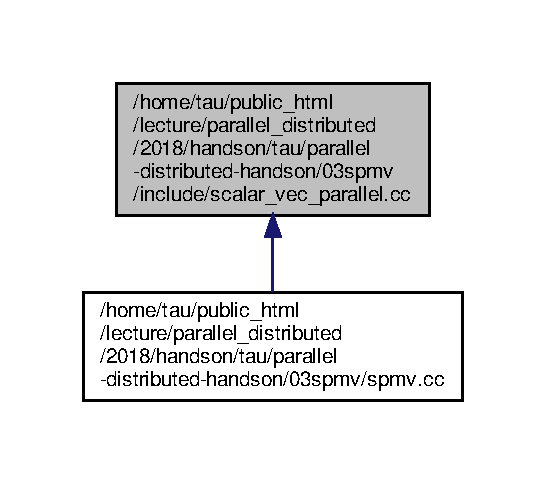
\includegraphics[width=262pt]{scalar__vec__parallel_8cc__dep__incl}
\end{center}
\end{figure}
\subsection*{Functions}
\begin{DoxyCompactItemize}
\item 
static int \hyperlink{scalar__vec__parallel_8cc_a26ccc7c1a9ee3268853441b1d0ce8f98}{scalar\+\_\+vec\+\_\+parallel} (\hyperlink{spmv_8cc_a11d147c64891830c9e79b3315b1b2e21}{real} k, \hyperlink{structvec__t}{vec\+\_\+t} v)
\begin{DoxyCompactList}\small\item\em k x v in parallel \end{DoxyCompactList}\end{DoxyCompactItemize}


\subsection{Detailed Description}
scalar x vector multiply with parallel for 



\subsection{Function Documentation}
\mbox{\Hypertarget{scalar__vec__parallel_8cc_a26ccc7c1a9ee3268853441b1d0ce8f98}\label{scalar__vec__parallel_8cc_a26ccc7c1a9ee3268853441b1d0ce8f98}} 
\index{scalar\+\_\+vec\+\_\+parallel.\+cc@{scalar\+\_\+vec\+\_\+parallel.\+cc}!scalar\+\_\+vec\+\_\+parallel@{scalar\+\_\+vec\+\_\+parallel}}
\index{scalar\+\_\+vec\+\_\+parallel@{scalar\+\_\+vec\+\_\+parallel}!scalar\+\_\+vec\+\_\+parallel.\+cc@{scalar\+\_\+vec\+\_\+parallel.\+cc}}
\subsubsection{\texorpdfstring{scalar\+\_\+vec\+\_\+parallel()}{scalar\_vec\_parallel()}}
{\footnotesize\ttfamily static int scalar\+\_\+vec\+\_\+parallel (\begin{DoxyParamCaption}\item[{\hyperlink{spmv_8cc_a11d147c64891830c9e79b3315b1b2e21}{real}}]{k,  }\item[{\hyperlink{structvec__t}{vec\+\_\+t}}]{v }\end{DoxyParamCaption})\hspace{0.3cm}{\ttfamily [static]}}



k x v in parallel 


\begin{DoxyParams}{Parameters}
{\em (k)} & a scalar \\
\hline
{\em (v)} & a vector \\
\hline
\end{DoxyParams}
\begin{DoxyReturn}{Returns}
1
\end{DoxyReturn}
multiply each element of v by k 
\hypertarget{scalar__vec__task_8cc}{}\section{/home/tau/public\+\_\+html/lecture/parallel\+\_\+distributed/2018/handson/tau/parallel-\/distributed-\/handson/03spmv/include/scalar\+\_\+vec\+\_\+task.cc File Reference}
\label{scalar__vec__task_8cc}\index{/home/tau/public\+\_\+html/lecture/parallel\+\_\+distributed/2018/handson/tau/parallel-\/distributed-\/handson/03spmv/include/scalar\+\_\+vec\+\_\+task.\+cc@{/home/tau/public\+\_\+html/lecture/parallel\+\_\+distributed/2018/handson/tau/parallel-\/distributed-\/handson/03spmv/include/scalar\+\_\+vec\+\_\+task.\+cc}}


scalar x vector multiply with tasks  


This graph shows which files directly or indirectly include this file\+:\nopagebreak
\begin{figure}[H]
\begin{center}
\leavevmode
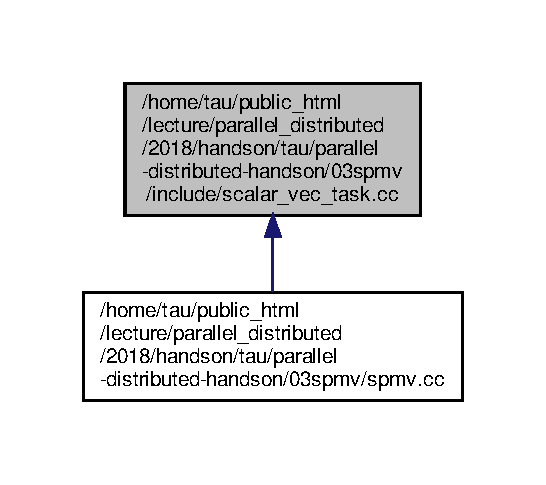
\includegraphics[width=262pt]{scalar__vec__task_8cc__dep__incl}
\end{center}
\end{figure}
\subsection*{Functions}
\begin{DoxyCompactItemize}
\item 
static int \hyperlink{scalar__vec__task_8cc_a7c173a211213a6c320853217b58e3a11}{scalar\+\_\+vec\+\_\+task} (\hyperlink{spmv_8cc_a11d147c64891830c9e79b3315b1b2e21}{real} k, \hyperlink{structvec__t}{vec\+\_\+t} v)
\begin{DoxyCompactList}\small\item\em k x v in parallel with tasks \end{DoxyCompactList}\end{DoxyCompactItemize}


\subsection{Detailed Description}
scalar x vector multiply with tasks 



\subsection{Function Documentation}
\mbox{\Hypertarget{scalar__vec__task_8cc_a7c173a211213a6c320853217b58e3a11}\label{scalar__vec__task_8cc_a7c173a211213a6c320853217b58e3a11}} 
\index{scalar\+\_\+vec\+\_\+task.\+cc@{scalar\+\_\+vec\+\_\+task.\+cc}!scalar\+\_\+vec\+\_\+task@{scalar\+\_\+vec\+\_\+task}}
\index{scalar\+\_\+vec\+\_\+task@{scalar\+\_\+vec\+\_\+task}!scalar\+\_\+vec\+\_\+task.\+cc@{scalar\+\_\+vec\+\_\+task.\+cc}}
\subsubsection{\texorpdfstring{scalar\+\_\+vec\+\_\+task()}{scalar\_vec\_task()}}
{\footnotesize\ttfamily static int scalar\+\_\+vec\+\_\+task (\begin{DoxyParamCaption}\item[{\hyperlink{spmv_8cc_a11d147c64891830c9e79b3315b1b2e21}{real}}]{k,  }\item[{\hyperlink{structvec__t}{vec\+\_\+t}}]{v }\end{DoxyParamCaption})\hspace{0.3cm}{\ttfamily [static]}}



k x v in parallel with tasks 


\begin{DoxyParams}{Parameters}
{\em (k)} & a scalar \\
\hline
{\em (v)} & a vector \\
\hline
\end{DoxyParams}
\begin{DoxyReturn}{Returns}
1
\end{DoxyReturn}
multiply each element of v by k 
\hypertarget{scalar__vec__udr_8cc}{}\section{/home/tau/public\+\_\+html/lecture/parallel\+\_\+distributed/2018/handson/tau/parallel-\/distributed-\/handson/03spmv/include/scalar\+\_\+vec\+\_\+udr.cc File Reference}
\label{scalar__vec__udr_8cc}\index{/home/tau/public\+\_\+html/lecture/parallel\+\_\+distributed/2018/handson/tau/parallel-\/distributed-\/handson/03spmv/include/scalar\+\_\+vec\+\_\+udr.\+cc@{/home/tau/public\+\_\+html/lecture/parallel\+\_\+distributed/2018/handson/tau/parallel-\/distributed-\/handson/03spmv/include/scalar\+\_\+vec\+\_\+udr.\+cc}}


scalar x vector multiply with parallel for + user-\/defined reductions  


This graph shows which files directly or indirectly include this file\+:\nopagebreak
\begin{figure}[H]
\begin{center}
\leavevmode
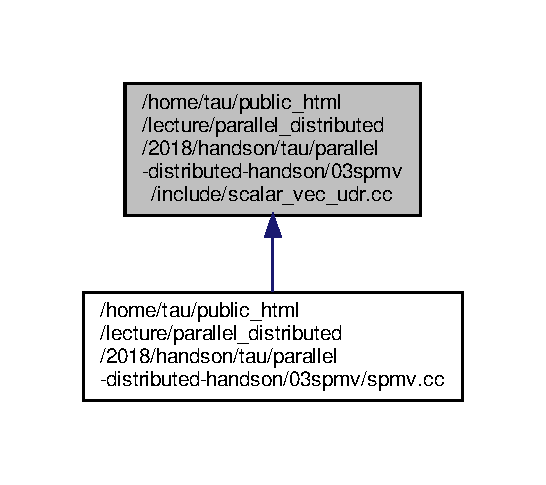
\includegraphics[width=262pt]{scalar__vec__udr_8cc__dep__incl}
\end{center}
\end{figure}
\subsection*{Functions}
\begin{DoxyCompactItemize}
\item 
static int \hyperlink{scalar__vec__udr_8cc_ad1461b5cf447013b133c040882692d3c}{scalar\+\_\+vec\+\_\+udr} (\hyperlink{spmv_8cc_a11d147c64891830c9e79b3315b1b2e21}{real} k, \hyperlink{structvec__t}{vec\+\_\+t} v)
\begin{DoxyCompactList}\small\item\em k x v in parallel with user-\/defined reductions \end{DoxyCompactList}\end{DoxyCompactItemize}


\subsection{Detailed Description}
scalar x vector multiply with parallel for + user-\/defined reductions 



\subsection{Function Documentation}
\mbox{\Hypertarget{scalar__vec__udr_8cc_ad1461b5cf447013b133c040882692d3c}\label{scalar__vec__udr_8cc_ad1461b5cf447013b133c040882692d3c}} 
\index{scalar\+\_\+vec\+\_\+udr.\+cc@{scalar\+\_\+vec\+\_\+udr.\+cc}!scalar\+\_\+vec\+\_\+udr@{scalar\+\_\+vec\+\_\+udr}}
\index{scalar\+\_\+vec\+\_\+udr@{scalar\+\_\+vec\+\_\+udr}!scalar\+\_\+vec\+\_\+udr.\+cc@{scalar\+\_\+vec\+\_\+udr.\+cc}}
\subsubsection{\texorpdfstring{scalar\+\_\+vec\+\_\+udr()}{scalar\_vec\_udr()}}
{\footnotesize\ttfamily static int scalar\+\_\+vec\+\_\+udr (\begin{DoxyParamCaption}\item[{\hyperlink{spmv_8cc_a11d147c64891830c9e79b3315b1b2e21}{real}}]{k,  }\item[{\hyperlink{structvec__t}{vec\+\_\+t}}]{v }\end{DoxyParamCaption})\hspace{0.3cm}{\ttfamily [static]}}



k x v in parallel with user-\/defined reductions 


\begin{DoxyParams}{Parameters}
{\em (k)} & a scalar \\
\hline
{\em (v)} & a vector \\
\hline
\end{DoxyParams}
\begin{DoxyReturn}{Returns}
1
\end{DoxyReturn}
multiply each element of v by k 
\hypertarget{spmv__coo__cuda_8cc}{}\section{/home/tau/public\+\_\+html/lecture/parallel\+\_\+distributed/2018/handson/tau/parallel-\/distributed-\/handson/03spmv/include/spmv\+\_\+coo\+\_\+cuda.cc File Reference}
\label{spmv__coo__cuda_8cc}\index{/home/tau/public\+\_\+html/lecture/parallel\+\_\+distributed/2018/handson/tau/parallel-\/distributed-\/handson/03spmv/include/spmv\+\_\+coo\+\_\+cuda.\+cc@{/home/tau/public\+\_\+html/lecture/parallel\+\_\+distributed/2018/handson/tau/parallel-\/distributed-\/handson/03spmv/include/spmv\+\_\+coo\+\_\+cuda.\+cc}}


y = A $\ast$ x for coo with cuda  


\subsection*{Functions}
\begin{DoxyCompactItemize}
\item 
\+\_\+\+\_\+global\+\_\+\+\_\+ void \hyperlink{spmv__coo__cuda_8cc_a38bf40a7fad355ba53f168a00c1f6b5a}{init\+\_\+const\+\_\+dev} (\hyperlink{structvec__t}{vec\+\_\+t} v, \hyperlink{spmv_8cc_a11d147c64891830c9e79b3315b1b2e21}{real} c)
\begin{DoxyCompactList}\small\item\em the device procedure to initialize all elements of v with a constant c \end{DoxyCompactList}\item 
\+\_\+\+\_\+global\+\_\+\+\_\+ void \hyperlink{spmv__coo__cuda_8cc_aa8b36d14695c5599ff6a2e724711101f}{spmv\+\_\+coo\+\_\+dev} (\hyperlink{structsparse__t}{sparse\+\_\+t} A, \hyperlink{structvec__t}{vec\+\_\+t} vx, \hyperlink{structvec__t}{vec\+\_\+t} vy)
\begin{DoxyCompactList}\small\item\em the device procedure to do spmv in coo format \end{DoxyCompactList}\item 
static int \hyperlink{spmv__coo__cuda_8cc_a0f69fc3347f24b8d0dff47851ba19aa4}{spmv\+\_\+coo\+\_\+cuda} (\hyperlink{structsparse__t}{sparse\+\_\+t} A, \hyperlink{structvec__t}{vec\+\_\+t} vx, \hyperlink{structvec__t}{vec\+\_\+t} vy)
\begin{DoxyCompactList}\small\item\em y = A $\ast$ x for coo with cuda \end{DoxyCompactList}\end{DoxyCompactItemize}


\subsection{Detailed Description}
y = A $\ast$ x for coo with cuda 



\subsection{Function Documentation}
\mbox{\Hypertarget{spmv__coo__cuda_8cc_a38bf40a7fad355ba53f168a00c1f6b5a}\label{spmv__coo__cuda_8cc_a38bf40a7fad355ba53f168a00c1f6b5a}} 
\index{spmv\+\_\+coo\+\_\+cuda.\+cc@{spmv\+\_\+coo\+\_\+cuda.\+cc}!init\+\_\+const\+\_\+dev@{init\+\_\+const\+\_\+dev}}
\index{init\+\_\+const\+\_\+dev@{init\+\_\+const\+\_\+dev}!spmv\+\_\+coo\+\_\+cuda.\+cc@{spmv\+\_\+coo\+\_\+cuda.\+cc}}
\subsubsection{\texorpdfstring{init\+\_\+const\+\_\+dev()}{init\_const\_dev()}}
{\footnotesize\ttfamily \+\_\+\+\_\+global\+\_\+\+\_\+ void init\+\_\+const\+\_\+dev (\begin{DoxyParamCaption}\item[{\hyperlink{structvec__t}{vec\+\_\+t}}]{v,  }\item[{\hyperlink{spmv_8cc_a11d147c64891830c9e79b3315b1b2e21}{real}}]{c }\end{DoxyParamCaption})}



the device procedure to initialize all elements of v with a constant c 


\begin{DoxyParams}{Parameters}
{\em (v)} & a vector \\
\hline
{\em (c)} & the value to initialize all v\textquotesingle{}s elements with \\
\hline
\end{DoxyParams}
\mbox{\Hypertarget{spmv__coo__cuda_8cc_a0f69fc3347f24b8d0dff47851ba19aa4}\label{spmv__coo__cuda_8cc_a0f69fc3347f24b8d0dff47851ba19aa4}} 
\index{spmv\+\_\+coo\+\_\+cuda.\+cc@{spmv\+\_\+coo\+\_\+cuda.\+cc}!spmv\+\_\+coo\+\_\+cuda@{spmv\+\_\+coo\+\_\+cuda}}
\index{spmv\+\_\+coo\+\_\+cuda@{spmv\+\_\+coo\+\_\+cuda}!spmv\+\_\+coo\+\_\+cuda.\+cc@{spmv\+\_\+coo\+\_\+cuda.\+cc}}
\subsubsection{\texorpdfstring{spmv\+\_\+coo\+\_\+cuda()}{spmv\_coo\_cuda()}}
{\footnotesize\ttfamily static int spmv\+\_\+coo\+\_\+cuda (\begin{DoxyParamCaption}\item[{\hyperlink{structsparse__t}{sparse\+\_\+t}}]{A,  }\item[{\hyperlink{structvec__t}{vec\+\_\+t}}]{vx,  }\item[{\hyperlink{structvec__t}{vec\+\_\+t}}]{vy }\end{DoxyParamCaption})\hspace{0.3cm}{\ttfamily [static]}}



y = A $\ast$ x for coo with cuda 


\begin{DoxyParams}{Parameters}
{\em (\+A)} & a sparse matrix in coo format \\
\hline
{\em (vx)} & a vector \\
\hline
{\em (vy)} & a vector \\
\hline
\end{DoxyParams}
\begin{DoxyReturn}{Returns}
1 if succeed, 0 if failed 
\end{DoxyReturn}
\mbox{\Hypertarget{spmv__coo__cuda_8cc_aa8b36d14695c5599ff6a2e724711101f}\label{spmv__coo__cuda_8cc_aa8b36d14695c5599ff6a2e724711101f}} 
\index{spmv\+\_\+coo\+\_\+cuda.\+cc@{spmv\+\_\+coo\+\_\+cuda.\+cc}!spmv\+\_\+coo\+\_\+dev@{spmv\+\_\+coo\+\_\+dev}}
\index{spmv\+\_\+coo\+\_\+dev@{spmv\+\_\+coo\+\_\+dev}!spmv\+\_\+coo\+\_\+cuda.\+cc@{spmv\+\_\+coo\+\_\+cuda.\+cc}}
\subsubsection{\texorpdfstring{spmv\+\_\+coo\+\_\+dev()}{spmv\_coo\_dev()}}
{\footnotesize\ttfamily \+\_\+\+\_\+global\+\_\+\+\_\+ void spmv\+\_\+coo\+\_\+dev (\begin{DoxyParamCaption}\item[{\hyperlink{structsparse__t}{sparse\+\_\+t}}]{A,  }\item[{\hyperlink{structvec__t}{vec\+\_\+t}}]{vx,  }\item[{\hyperlink{structvec__t}{vec\+\_\+t}}]{vy }\end{DoxyParamCaption})}



the device procedure to do spmv in coo format 


\begin{DoxyParams}{Parameters}
{\em (\+A)} & a sparse matrix \\
\hline
{\em (vx)} & a vector \\
\hline
{\em (vy)} & a vector\\
\hline
\end{DoxyParams}
assume A, vx, vy must have their elems\+\_\+dev already set. 
\hypertarget{spmv__coo__parallel_8cc}{}\section{/home/tau/public\+\_\+html/lecture/parallel\+\_\+distributed/2018/handson/tau/parallel-\/distributed-\/handson/03spmv/include/spmv\+\_\+coo\+\_\+parallel.cc File Reference}
\label{spmv__coo__parallel_8cc}\index{/home/tau/public\+\_\+html/lecture/parallel\+\_\+distributed/2018/handson/tau/parallel-\/distributed-\/handson/03spmv/include/spmv\+\_\+coo\+\_\+parallel.\+cc@{/home/tau/public\+\_\+html/lecture/parallel\+\_\+distributed/2018/handson/tau/parallel-\/distributed-\/handson/03spmv/include/spmv\+\_\+coo\+\_\+parallel.\+cc}}


y = A $\ast$ x for coo with parallel for  


This graph shows which files directly or indirectly include this file\+:\nopagebreak
\begin{figure}[H]
\begin{center}
\leavevmode
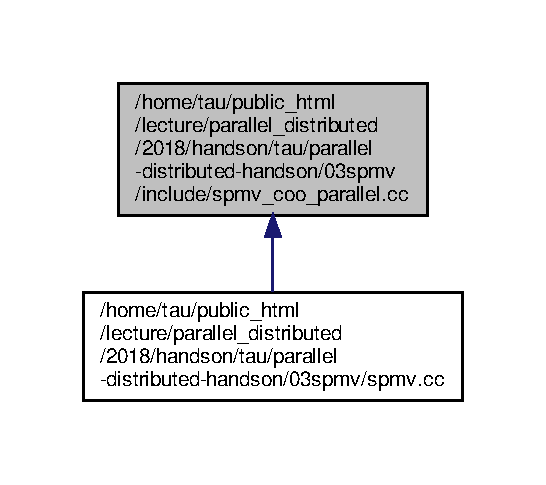
\includegraphics[width=262pt]{spmv__coo__parallel_8cc__dep__incl}
\end{center}
\end{figure}
\subsection*{Functions}
\begin{DoxyCompactItemize}
\item 
static int \hyperlink{spmv__coo__parallel_8cc_ada3d431757871be30e0fe48b89a33973}{spmv\+\_\+coo\+\_\+parallel} (\hyperlink{structsparse__t}{sparse\+\_\+t} A, \hyperlink{structvec__t}{vec\+\_\+t} vx, \hyperlink{structvec__t}{vec\+\_\+t} vy)
\begin{DoxyCompactList}\small\item\em y = A $\ast$ x for coo with parallel for \end{DoxyCompactList}\end{DoxyCompactItemize}


\subsection{Detailed Description}
y = A $\ast$ x for coo with parallel for 



\subsection{Function Documentation}
\mbox{\Hypertarget{spmv__coo__parallel_8cc_ada3d431757871be30e0fe48b89a33973}\label{spmv__coo__parallel_8cc_ada3d431757871be30e0fe48b89a33973}} 
\index{spmv\+\_\+coo\+\_\+parallel.\+cc@{spmv\+\_\+coo\+\_\+parallel.\+cc}!spmv\+\_\+coo\+\_\+parallel@{spmv\+\_\+coo\+\_\+parallel}}
\index{spmv\+\_\+coo\+\_\+parallel@{spmv\+\_\+coo\+\_\+parallel}!spmv\+\_\+coo\+\_\+parallel.\+cc@{spmv\+\_\+coo\+\_\+parallel.\+cc}}
\subsubsection{\texorpdfstring{spmv\+\_\+coo\+\_\+parallel()}{spmv\_coo\_parallel()}}
{\footnotesize\ttfamily static int spmv\+\_\+coo\+\_\+parallel (\begin{DoxyParamCaption}\item[{\hyperlink{structsparse__t}{sparse\+\_\+t}}]{A,  }\item[{\hyperlink{structvec__t}{vec\+\_\+t}}]{vx,  }\item[{\hyperlink{structvec__t}{vec\+\_\+t}}]{vy }\end{DoxyParamCaption})\hspace{0.3cm}{\ttfamily [static]}}



y = A $\ast$ x for coo with parallel for 


\begin{DoxyParams}{Parameters}
{\em (\+A)} & a sparse matrix \\
\hline
{\em (vx)} & a vector \\
\hline
{\em (vy)} & a vector \\
\hline
\end{DoxyParams}
\begin{DoxyReturn}{Returns}
1 if succeed, 0 if failed 
\end{DoxyReturn}

\hypertarget{spmv__coo__sorted__cuda_8cc}{}\section{/home/tau/public\+\_\+html/lecture/parallel\+\_\+distributed/2018/handson/tau/parallel-\/distributed-\/handson/03spmv/include/spmv\+\_\+coo\+\_\+sorted\+\_\+cuda.cc File Reference}
\label{spmv__coo__sorted__cuda_8cc}\index{/home/tau/public\+\_\+html/lecture/parallel\+\_\+distributed/2018/handson/tau/parallel-\/distributed-\/handson/03spmv/include/spmv\+\_\+coo\+\_\+sorted\+\_\+cuda.\+cc@{/home/tau/public\+\_\+html/lecture/parallel\+\_\+distributed/2018/handson/tau/parallel-\/distributed-\/handson/03spmv/include/spmv\+\_\+coo\+\_\+sorted\+\_\+cuda.\+cc}}


y = A $\ast$ x for coo\+\_\+sorted with cuda  


\subsection*{Functions}
\begin{DoxyCompactItemize}
\item 
static int \hyperlink{spmv__coo__sorted__cuda_8cc_a0c7f09dff7ec7a603acd26a19a44450d}{spmv\+\_\+coo\+\_\+sorted\+\_\+cuda} (\hyperlink{structsparse__t}{sparse\+\_\+t} A, \hyperlink{structvec__t}{vec\+\_\+t} vx, \hyperlink{structvec__t}{vec\+\_\+t} vy)
\begin{DoxyCompactList}\small\item\em y = A $\ast$ x for coo\+\_\+sorted with cuda \end{DoxyCompactList}\end{DoxyCompactItemize}


\subsection{Detailed Description}
y = A $\ast$ x for coo\+\_\+sorted with cuda 



\subsection{Function Documentation}
\mbox{\Hypertarget{spmv__coo__sorted__cuda_8cc_a0c7f09dff7ec7a603acd26a19a44450d}\label{spmv__coo__sorted__cuda_8cc_a0c7f09dff7ec7a603acd26a19a44450d}} 
\index{spmv\+\_\+coo\+\_\+sorted\+\_\+cuda.\+cc@{spmv\+\_\+coo\+\_\+sorted\+\_\+cuda.\+cc}!spmv\+\_\+coo\+\_\+sorted\+\_\+cuda@{spmv\+\_\+coo\+\_\+sorted\+\_\+cuda}}
\index{spmv\+\_\+coo\+\_\+sorted\+\_\+cuda@{spmv\+\_\+coo\+\_\+sorted\+\_\+cuda}!spmv\+\_\+coo\+\_\+sorted\+\_\+cuda.\+cc@{spmv\+\_\+coo\+\_\+sorted\+\_\+cuda.\+cc}}
\subsubsection{\texorpdfstring{spmv\+\_\+coo\+\_\+sorted\+\_\+cuda()}{spmv\_coo\_sorted\_cuda()}}
{\footnotesize\ttfamily static int spmv\+\_\+coo\+\_\+sorted\+\_\+cuda (\begin{DoxyParamCaption}\item[{\hyperlink{structsparse__t}{sparse\+\_\+t}}]{A,  }\item[{\hyperlink{structvec__t}{vec\+\_\+t}}]{vx,  }\item[{\hyperlink{structvec__t}{vec\+\_\+t}}]{vy }\end{DoxyParamCaption})\hspace{0.3cm}{\ttfamily [static]}}



y = A $\ast$ x for coo\+\_\+sorted with cuda 


\begin{DoxyParams}{Parameters}
{\em (\+A)} & a sparse matrix \\
\hline
{\em (vx)} & a vector \\
\hline
{\em (vy)} & a vector \\
\hline
\end{DoxyParams}
\begin{DoxyReturn}{Returns}
1 if succeed, 0 if failed 
\end{DoxyReturn}

\hypertarget{spmv__coo__sorted__parallel_8cc}{}\section{/home/tau/public\+\_\+html/lecture/parallel\+\_\+distributed/2018/handson/tau/parallel-\/distributed-\/handson/03spmv/include/spmv\+\_\+coo\+\_\+sorted\+\_\+parallel.cc File Reference}
\label{spmv__coo__sorted__parallel_8cc}\index{/home/tau/public\+\_\+html/lecture/parallel\+\_\+distributed/2018/handson/tau/parallel-\/distributed-\/handson/03spmv/include/spmv\+\_\+coo\+\_\+sorted\+\_\+parallel.\+cc@{/home/tau/public\+\_\+html/lecture/parallel\+\_\+distributed/2018/handson/tau/parallel-\/distributed-\/handson/03spmv/include/spmv\+\_\+coo\+\_\+sorted\+\_\+parallel.\+cc}}


y = A $\ast$ x for coo\+\_\+sorted with parallel for  


This graph shows which files directly or indirectly include this file\+:\nopagebreak
\begin{figure}[H]
\begin{center}
\leavevmode
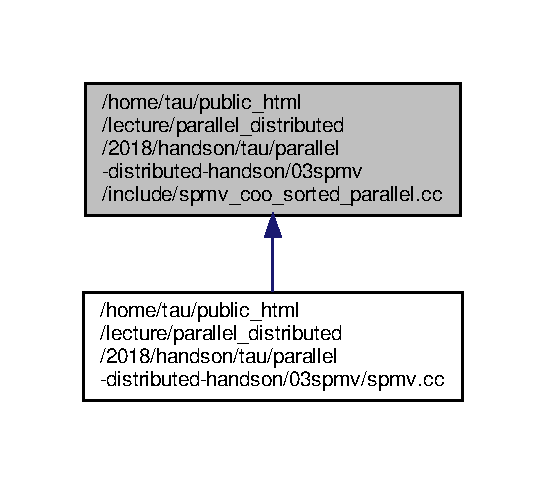
\includegraphics[width=262pt]{spmv__coo__sorted__parallel_8cc__dep__incl}
\end{center}
\end{figure}
\subsection*{Functions}
\begin{DoxyCompactItemize}
\item 
static int \hyperlink{spmv__coo__sorted__parallel_8cc_a288772ff3dade2ab26450de5349b2d10}{spmv\+\_\+coo\+\_\+sorted\+\_\+parallel} (\hyperlink{structsparse__t}{sparse\+\_\+t} A, \hyperlink{structvec__t}{vec\+\_\+t} vx, \hyperlink{structvec__t}{vec\+\_\+t} vy)
\begin{DoxyCompactList}\small\item\em y = A $\ast$ x for coo\+\_\+sorted with parallel for \end{DoxyCompactList}\end{DoxyCompactItemize}


\subsection{Detailed Description}
y = A $\ast$ x for coo\+\_\+sorted with parallel for 



\subsection{Function Documentation}
\mbox{\Hypertarget{spmv__coo__sorted__parallel_8cc_a288772ff3dade2ab26450de5349b2d10}\label{spmv__coo__sorted__parallel_8cc_a288772ff3dade2ab26450de5349b2d10}} 
\index{spmv\+\_\+coo\+\_\+sorted\+\_\+parallel.\+cc@{spmv\+\_\+coo\+\_\+sorted\+\_\+parallel.\+cc}!spmv\+\_\+coo\+\_\+sorted\+\_\+parallel@{spmv\+\_\+coo\+\_\+sorted\+\_\+parallel}}
\index{spmv\+\_\+coo\+\_\+sorted\+\_\+parallel@{spmv\+\_\+coo\+\_\+sorted\+\_\+parallel}!spmv\+\_\+coo\+\_\+sorted\+\_\+parallel.\+cc@{spmv\+\_\+coo\+\_\+sorted\+\_\+parallel.\+cc}}
\subsubsection{\texorpdfstring{spmv\+\_\+coo\+\_\+sorted\+\_\+parallel()}{spmv\_coo\_sorted\_parallel()}}
{\footnotesize\ttfamily static int spmv\+\_\+coo\+\_\+sorted\+\_\+parallel (\begin{DoxyParamCaption}\item[{\hyperlink{structsparse__t}{sparse\+\_\+t}}]{A,  }\item[{\hyperlink{structvec__t}{vec\+\_\+t}}]{vx,  }\item[{\hyperlink{structvec__t}{vec\+\_\+t}}]{vy }\end{DoxyParamCaption})\hspace{0.3cm}{\ttfamily [static]}}



y = A $\ast$ x for coo\+\_\+sorted with parallel for 


\begin{DoxyParams}{Parameters}
{\em (\+A)} & a sparse matrix \\
\hline
{\em (vx)} & a vector \\
\hline
{\em (vy)} & a vector \\
\hline
\end{DoxyParams}
\begin{DoxyReturn}{Returns}
1 if succeed, 0 if failed 
\end{DoxyReturn}

\hypertarget{spmv__coo__sorted__task_8cc}{}\section{/home/tau/public\+\_\+html/lecture/parallel\+\_\+distributed/2018/handson/tau/parallel-\/distributed-\/handson/03spmv/include/spmv\+\_\+coo\+\_\+sorted\+\_\+task.cc File Reference}
\label{spmv__coo__sorted__task_8cc}\index{/home/tau/public\+\_\+html/lecture/parallel\+\_\+distributed/2018/handson/tau/parallel-\/distributed-\/handson/03spmv/include/spmv\+\_\+coo\+\_\+sorted\+\_\+task.\+cc@{/home/tau/public\+\_\+html/lecture/parallel\+\_\+distributed/2018/handson/tau/parallel-\/distributed-\/handson/03spmv/include/spmv\+\_\+coo\+\_\+sorted\+\_\+task.\+cc}}


y = A $\ast$ x with tasks for coo\+\_\+sorted  


This graph shows which files directly or indirectly include this file\+:\nopagebreak
\begin{figure}[H]
\begin{center}
\leavevmode
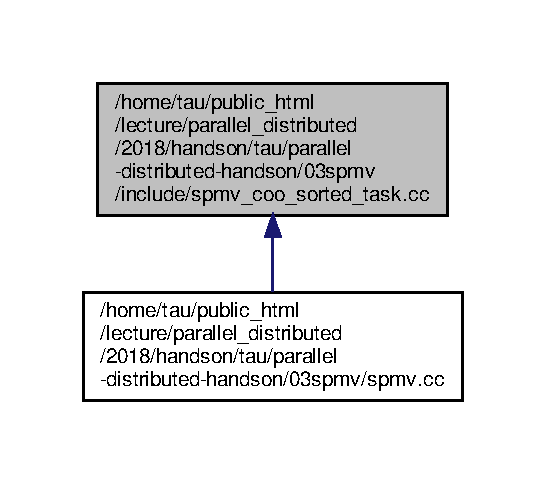
\includegraphics[width=262pt]{spmv__coo__sorted__task_8cc__dep__incl}
\end{center}
\end{figure}
\subsection*{Functions}
\begin{DoxyCompactItemize}
\item 
static int \hyperlink{spmv__coo__sorted__task_8cc_a54003161e4ed3de194a75c43ae8338d4}{spmv\+\_\+coo\+\_\+sorted\+\_\+task} (\hyperlink{structsparse__t}{sparse\+\_\+t} A, \hyperlink{structvec__t}{vec\+\_\+t} vx, \hyperlink{structvec__t}{vec\+\_\+t} vy)
\begin{DoxyCompactList}\small\item\em y = A $\ast$ x with tasks for coo\+\_\+sorted \end{DoxyCompactList}\end{DoxyCompactItemize}


\subsection{Detailed Description}
y = A $\ast$ x with tasks for coo\+\_\+sorted 



\subsection{Function Documentation}
\mbox{\Hypertarget{spmv__coo__sorted__task_8cc_a54003161e4ed3de194a75c43ae8338d4}\label{spmv__coo__sorted__task_8cc_a54003161e4ed3de194a75c43ae8338d4}} 
\index{spmv\+\_\+coo\+\_\+sorted\+\_\+task.\+cc@{spmv\+\_\+coo\+\_\+sorted\+\_\+task.\+cc}!spmv\+\_\+coo\+\_\+sorted\+\_\+task@{spmv\+\_\+coo\+\_\+sorted\+\_\+task}}
\index{spmv\+\_\+coo\+\_\+sorted\+\_\+task@{spmv\+\_\+coo\+\_\+sorted\+\_\+task}!spmv\+\_\+coo\+\_\+sorted\+\_\+task.\+cc@{spmv\+\_\+coo\+\_\+sorted\+\_\+task.\+cc}}
\subsubsection{\texorpdfstring{spmv\+\_\+coo\+\_\+sorted\+\_\+task()}{spmv\_coo\_sorted\_task()}}
{\footnotesize\ttfamily static int spmv\+\_\+coo\+\_\+sorted\+\_\+task (\begin{DoxyParamCaption}\item[{\hyperlink{structsparse__t}{sparse\+\_\+t}}]{A,  }\item[{\hyperlink{structvec__t}{vec\+\_\+t}}]{vx,  }\item[{\hyperlink{structvec__t}{vec\+\_\+t}}]{vy }\end{DoxyParamCaption})\hspace{0.3cm}{\ttfamily [static]}}



y = A $\ast$ x with tasks for coo\+\_\+sorted 


\begin{DoxyParams}{Parameters}
{\em (\+A)} & a sparse matrix \\
\hline
{\em (vx)} & a vector \\
\hline
{\em (vy)} & a vector \\
\hline
\end{DoxyParams}
\begin{DoxyReturn}{Returns}
1 if succeed, 0 if failed 
\end{DoxyReturn}

\hypertarget{spmv__coo__sorted__udr_8cc}{}\section{/home/tau/public\+\_\+html/lecture/parallel\+\_\+distributed/2018/handson/tau/parallel-\/distributed-\/handson/03spmv/include/spmv\+\_\+coo\+\_\+sorted\+\_\+udr.cc File Reference}
\label{spmv__coo__sorted__udr_8cc}\index{/home/tau/public\+\_\+html/lecture/parallel\+\_\+distributed/2018/handson/tau/parallel-\/distributed-\/handson/03spmv/include/spmv\+\_\+coo\+\_\+sorted\+\_\+udr.\+cc@{/home/tau/public\+\_\+html/lecture/parallel\+\_\+distributed/2018/handson/tau/parallel-\/distributed-\/handson/03spmv/include/spmv\+\_\+coo\+\_\+sorted\+\_\+udr.\+cc}}


y = A $\ast$ x for coo\+\_\+sorted with parallel for + user-\/defined reductions  


This graph shows which files directly or indirectly include this file\+:\nopagebreak
\begin{figure}[H]
\begin{center}
\leavevmode
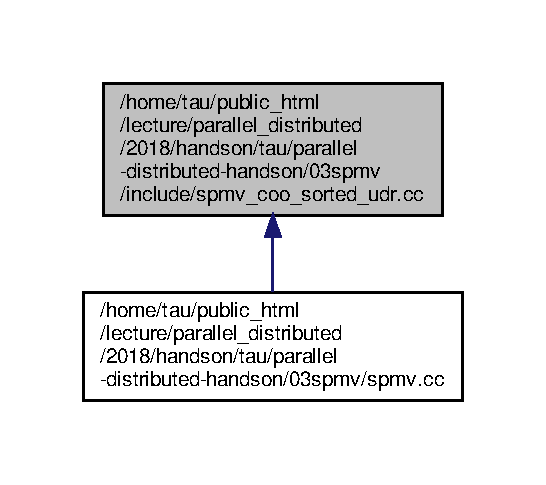
\includegraphics[width=262pt]{spmv__coo__sorted__udr_8cc__dep__incl}
\end{center}
\end{figure}
\subsection*{Functions}
\begin{DoxyCompactItemize}
\item 
static int \hyperlink{spmv__coo__sorted__udr_8cc_acd8cf86cbdc5f244e2e28364e73e4ce9}{spmv\+\_\+coo\+\_\+sorted\+\_\+udr} (\hyperlink{structsparse__t}{sparse\+\_\+t} A, \hyperlink{structvec__t}{vec\+\_\+t} vx, \hyperlink{structvec__t}{vec\+\_\+t} vy)
\begin{DoxyCompactList}\small\item\em y = A $\ast$ x for coo\+\_\+sorted with parallel for + user-\/defined reductions \end{DoxyCompactList}\end{DoxyCompactItemize}


\subsection{Detailed Description}
y = A $\ast$ x for coo\+\_\+sorted with parallel for + user-\/defined reductions 



\subsection{Function Documentation}
\mbox{\Hypertarget{spmv__coo__sorted__udr_8cc_acd8cf86cbdc5f244e2e28364e73e4ce9}\label{spmv__coo__sorted__udr_8cc_acd8cf86cbdc5f244e2e28364e73e4ce9}} 
\index{spmv\+\_\+coo\+\_\+sorted\+\_\+udr.\+cc@{spmv\+\_\+coo\+\_\+sorted\+\_\+udr.\+cc}!spmv\+\_\+coo\+\_\+sorted\+\_\+udr@{spmv\+\_\+coo\+\_\+sorted\+\_\+udr}}
\index{spmv\+\_\+coo\+\_\+sorted\+\_\+udr@{spmv\+\_\+coo\+\_\+sorted\+\_\+udr}!spmv\+\_\+coo\+\_\+sorted\+\_\+udr.\+cc@{spmv\+\_\+coo\+\_\+sorted\+\_\+udr.\+cc}}
\subsubsection{\texorpdfstring{spmv\+\_\+coo\+\_\+sorted\+\_\+udr()}{spmv\_coo\_sorted\_udr()}}
{\footnotesize\ttfamily static int spmv\+\_\+coo\+\_\+sorted\+\_\+udr (\begin{DoxyParamCaption}\item[{\hyperlink{structsparse__t}{sparse\+\_\+t}}]{A,  }\item[{\hyperlink{structvec__t}{vec\+\_\+t}}]{vx,  }\item[{\hyperlink{structvec__t}{vec\+\_\+t}}]{vy }\end{DoxyParamCaption})\hspace{0.3cm}{\ttfamily [static]}}



y = A $\ast$ x for coo\+\_\+sorted with parallel for + user-\/defined reductions 


\begin{DoxyParams}{Parameters}
{\em (\+A)} & a sparse matrix \\
\hline
{\em (vx)} & a vector \\
\hline
{\em (vy)} & a vector \\
\hline
\end{DoxyParams}
\begin{DoxyReturn}{Returns}
1 if succeed, 0 if failed 
\end{DoxyReturn}

\hypertarget{spmv__coo__task_8cc}{}\section{/home/tau/public\+\_\+html/lecture/parallel\+\_\+distributed/2018/handson/tau/parallel-\/distributed-\/handson/03spmv/include/spmv\+\_\+coo\+\_\+task.cc File Reference}
\label{spmv__coo__task_8cc}\index{/home/tau/public\+\_\+html/lecture/parallel\+\_\+distributed/2018/handson/tau/parallel-\/distributed-\/handson/03spmv/include/spmv\+\_\+coo\+\_\+task.\+cc@{/home/tau/public\+\_\+html/lecture/parallel\+\_\+distributed/2018/handson/tau/parallel-\/distributed-\/handson/03spmv/include/spmv\+\_\+coo\+\_\+task.\+cc}}


y = A $\ast$ x for coo with tasks  


This graph shows which files directly or indirectly include this file\+:\nopagebreak
\begin{figure}[H]
\begin{center}
\leavevmode
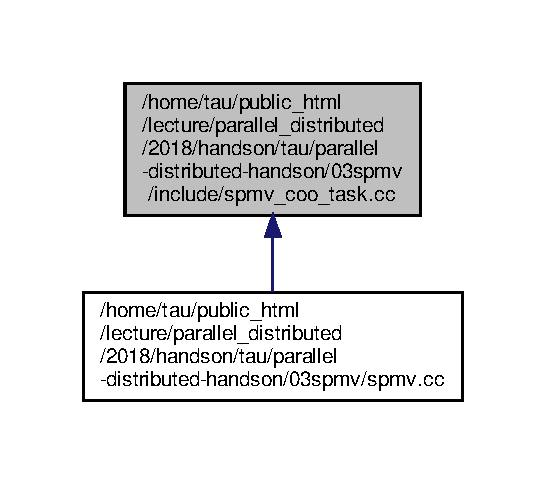
\includegraphics[width=262pt]{spmv__coo__task_8cc__dep__incl}
\end{center}
\end{figure}
\subsection*{Functions}
\begin{DoxyCompactItemize}
\item 
static int \hyperlink{spmv__coo__task_8cc_a0a02ba419ed338501ccf990bb7019429}{spmv\+\_\+coo\+\_\+task} (\hyperlink{structsparse__t}{sparse\+\_\+t} A, \hyperlink{structvec__t}{vec\+\_\+t} vx, \hyperlink{structvec__t}{vec\+\_\+t} vy)
\begin{DoxyCompactList}\small\item\em y = A $\ast$ x for coo with tasks \end{DoxyCompactList}\end{DoxyCompactItemize}


\subsection{Detailed Description}
y = A $\ast$ x for coo with tasks 



\subsection{Function Documentation}
\mbox{\Hypertarget{spmv__coo__task_8cc_a0a02ba419ed338501ccf990bb7019429}\label{spmv__coo__task_8cc_a0a02ba419ed338501ccf990bb7019429}} 
\index{spmv\+\_\+coo\+\_\+task.\+cc@{spmv\+\_\+coo\+\_\+task.\+cc}!spmv\+\_\+coo\+\_\+task@{spmv\+\_\+coo\+\_\+task}}
\index{spmv\+\_\+coo\+\_\+task@{spmv\+\_\+coo\+\_\+task}!spmv\+\_\+coo\+\_\+task.\+cc@{spmv\+\_\+coo\+\_\+task.\+cc}}
\subsubsection{\texorpdfstring{spmv\+\_\+coo\+\_\+task()}{spmv\_coo\_task()}}
{\footnotesize\ttfamily static int spmv\+\_\+coo\+\_\+task (\begin{DoxyParamCaption}\item[{\hyperlink{structsparse__t}{sparse\+\_\+t}}]{A,  }\item[{\hyperlink{structvec__t}{vec\+\_\+t}}]{vx,  }\item[{\hyperlink{structvec__t}{vec\+\_\+t}}]{vy }\end{DoxyParamCaption})\hspace{0.3cm}{\ttfamily [static]}}



y = A $\ast$ x for coo with tasks 


\begin{DoxyParams}{Parameters}
{\em (\+A)} & a sparse matrix \\
\hline
{\em (vx)} & a vector \\
\hline
{\em (vy)} & a vector \\
\hline
\end{DoxyParams}
\begin{DoxyReturn}{Returns}
1 if succeed, 0 if failed 
\end{DoxyReturn}

\hypertarget{spmv__coo__udr_8cc}{}\section{/home/tau/public\+\_\+html/lecture/parallel\+\_\+distributed/2018/handson/tau/parallel-\/distributed-\/handson/03spmv/include/spmv\+\_\+coo\+\_\+udr.cc File Reference}
\label{spmv__coo__udr_8cc}\index{/home/tau/public\+\_\+html/lecture/parallel\+\_\+distributed/2018/handson/tau/parallel-\/distributed-\/handson/03spmv/include/spmv\+\_\+coo\+\_\+udr.\+cc@{/home/tau/public\+\_\+html/lecture/parallel\+\_\+distributed/2018/handson/tau/parallel-\/distributed-\/handson/03spmv/include/spmv\+\_\+coo\+\_\+udr.\+cc}}


y = A $\ast$ x for coo with parallel for + user-\/defined reductions  


This graph shows which files directly or indirectly include this file\+:\nopagebreak
\begin{figure}[H]
\begin{center}
\leavevmode
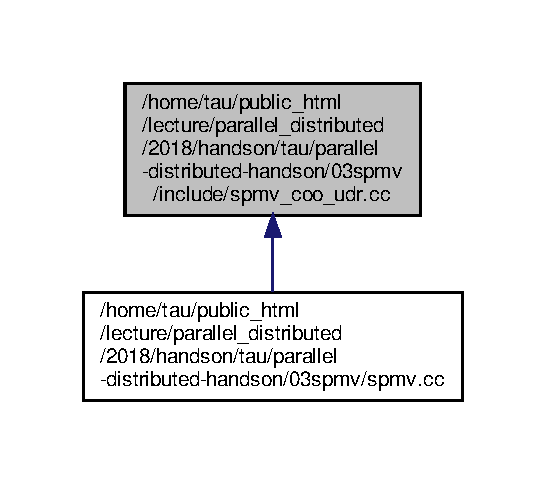
\includegraphics[width=262pt]{spmv__coo__udr_8cc__dep__incl}
\end{center}
\end{figure}
\subsection*{Functions}
\begin{DoxyCompactItemize}
\item 
static int \hyperlink{spmv__coo__udr_8cc_ac0d55e45d8bdc6031dc8d948da81b12c}{spmv\+\_\+coo\+\_\+udr} (\hyperlink{structsparse__t}{sparse\+\_\+t} A, \hyperlink{structvec__t}{vec\+\_\+t} vx, \hyperlink{structvec__t}{vec\+\_\+t} vy)
\begin{DoxyCompactList}\small\item\em y = A $\ast$ x for coo with parallel for + user-\/defined reductions \end{DoxyCompactList}\end{DoxyCompactItemize}


\subsection{Detailed Description}
y = A $\ast$ x for coo with parallel for + user-\/defined reductions 



\subsection{Function Documentation}
\mbox{\Hypertarget{spmv__coo__udr_8cc_ac0d55e45d8bdc6031dc8d948da81b12c}\label{spmv__coo__udr_8cc_ac0d55e45d8bdc6031dc8d948da81b12c}} 
\index{spmv\+\_\+coo\+\_\+udr.\+cc@{spmv\+\_\+coo\+\_\+udr.\+cc}!spmv\+\_\+coo\+\_\+udr@{spmv\+\_\+coo\+\_\+udr}}
\index{spmv\+\_\+coo\+\_\+udr@{spmv\+\_\+coo\+\_\+udr}!spmv\+\_\+coo\+\_\+udr.\+cc@{spmv\+\_\+coo\+\_\+udr.\+cc}}
\subsubsection{\texorpdfstring{spmv\+\_\+coo\+\_\+udr()}{spmv\_coo\_udr()}}
{\footnotesize\ttfamily static int spmv\+\_\+coo\+\_\+udr (\begin{DoxyParamCaption}\item[{\hyperlink{structsparse__t}{sparse\+\_\+t}}]{A,  }\item[{\hyperlink{structvec__t}{vec\+\_\+t}}]{vx,  }\item[{\hyperlink{structvec__t}{vec\+\_\+t}}]{vy }\end{DoxyParamCaption})\hspace{0.3cm}{\ttfamily [static]}}



y = A $\ast$ x for coo with parallel for + user-\/defined reductions 


\begin{DoxyParams}{Parameters}
{\em (\+A)} & a sparse matrix \\
\hline
{\em (vx)} & a vector \\
\hline
{\em (vy)} & a vector \\
\hline
\end{DoxyParams}
\begin{DoxyReturn}{Returns}
1 if succeed, 0 if failed 
\end{DoxyReturn}

\hypertarget{spmv__csr__cuda_8cc}{}\section{/home/tau/public\+\_\+html/lecture/parallel\+\_\+distributed/2018/handson/tau/parallel-\/distributed-\/handson/03spmv/include/spmv\+\_\+csr\+\_\+cuda.cc File Reference}
\label{spmv__csr__cuda_8cc}\index{/home/tau/public\+\_\+html/lecture/parallel\+\_\+distributed/2018/handson/tau/parallel-\/distributed-\/handson/03spmv/include/spmv\+\_\+csr\+\_\+cuda.\+cc@{/home/tau/public\+\_\+html/lecture/parallel\+\_\+distributed/2018/handson/tau/parallel-\/distributed-\/handson/03spmv/include/spmv\+\_\+csr\+\_\+cuda.\+cc}}


y = A $\ast$ x for csr with cuda  


\subsection*{Functions}
\begin{DoxyCompactItemize}
\item 
static int \hyperlink{spmv__csr__cuda_8cc_abfe0e8ff9d93cc6da3bbe47f3f9b8ea9}{spmv\+\_\+csr\+\_\+cuda} (\hyperlink{structsparse__t}{sparse\+\_\+t} A, \hyperlink{structvec__t}{vec\+\_\+t} vx, \hyperlink{structvec__t}{vec\+\_\+t} vy)
\begin{DoxyCompactList}\small\item\em y = A $\ast$ x for csr with cuda \end{DoxyCompactList}\end{DoxyCompactItemize}


\subsection{Detailed Description}
y = A $\ast$ x for csr with cuda 



\subsection{Function Documentation}
\mbox{\Hypertarget{spmv__csr__cuda_8cc_abfe0e8ff9d93cc6da3bbe47f3f9b8ea9}\label{spmv__csr__cuda_8cc_abfe0e8ff9d93cc6da3bbe47f3f9b8ea9}} 
\index{spmv\+\_\+csr\+\_\+cuda.\+cc@{spmv\+\_\+csr\+\_\+cuda.\+cc}!spmv\+\_\+csr\+\_\+cuda@{spmv\+\_\+csr\+\_\+cuda}}
\index{spmv\+\_\+csr\+\_\+cuda@{spmv\+\_\+csr\+\_\+cuda}!spmv\+\_\+csr\+\_\+cuda.\+cc@{spmv\+\_\+csr\+\_\+cuda.\+cc}}
\subsubsection{\texorpdfstring{spmv\+\_\+csr\+\_\+cuda()}{spmv\_csr\_cuda()}}
{\footnotesize\ttfamily static int spmv\+\_\+csr\+\_\+cuda (\begin{DoxyParamCaption}\item[{\hyperlink{structsparse__t}{sparse\+\_\+t}}]{A,  }\item[{\hyperlink{structvec__t}{vec\+\_\+t}}]{vx,  }\item[{\hyperlink{structvec__t}{vec\+\_\+t}}]{vy }\end{DoxyParamCaption})\hspace{0.3cm}{\ttfamily [static]}}



y = A $\ast$ x for csr with cuda 


\begin{DoxyParams}{Parameters}
{\em (\+A)} & a sparse matrix \\
\hline
{\em (vx)} & a vector \\
\hline
{\em (vy)} & a vector \\
\hline
\end{DoxyParams}
\begin{DoxyReturn}{Returns}
1 if succeed, 0 if failed 
\end{DoxyReturn}

\hypertarget{spmv__csr__parallel_8cc}{}\section{/home/tau/public\+\_\+html/lecture/parallel\+\_\+distributed/2018/handson/tau/parallel-\/distributed-\/handson/03spmv/include/spmv\+\_\+csr\+\_\+parallel.cc File Reference}
\label{spmv__csr__parallel_8cc}\index{/home/tau/public\+\_\+html/lecture/parallel\+\_\+distributed/2018/handson/tau/parallel-\/distributed-\/handson/03spmv/include/spmv\+\_\+csr\+\_\+parallel.\+cc@{/home/tau/public\+\_\+html/lecture/parallel\+\_\+distributed/2018/handson/tau/parallel-\/distributed-\/handson/03spmv/include/spmv\+\_\+csr\+\_\+parallel.\+cc}}


y = A $\ast$ x for csr with parallel for  


This graph shows which files directly or indirectly include this file\+:\nopagebreak
\begin{figure}[H]
\begin{center}
\leavevmode
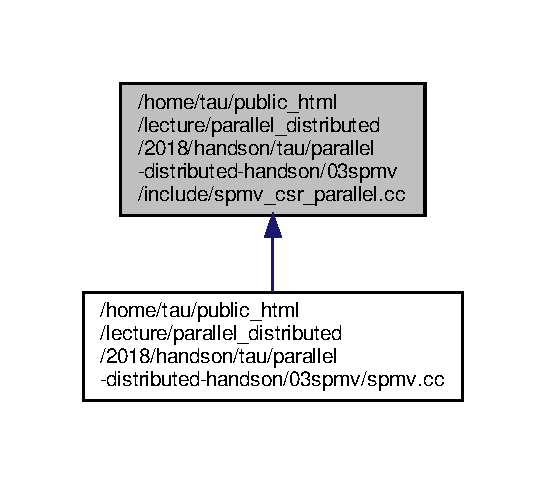
\includegraphics[width=262pt]{spmv__csr__parallel_8cc__dep__incl}
\end{center}
\end{figure}
\subsection*{Functions}
\begin{DoxyCompactItemize}
\item 
static int \hyperlink{spmv__csr__parallel_8cc_ae2c3871d937f3d196bfe193737ef2185}{spmv\+\_\+csr\+\_\+parallel} (\hyperlink{structsparse__t}{sparse\+\_\+t} A, \hyperlink{structvec__t}{vec\+\_\+t} vx, \hyperlink{structvec__t}{vec\+\_\+t} vy)
\begin{DoxyCompactList}\small\item\em y = A $\ast$ x for csr with parallel for \end{DoxyCompactList}\end{DoxyCompactItemize}


\subsection{Detailed Description}
y = A $\ast$ x for csr with parallel for 



\subsection{Function Documentation}
\mbox{\Hypertarget{spmv__csr__parallel_8cc_ae2c3871d937f3d196bfe193737ef2185}\label{spmv__csr__parallel_8cc_ae2c3871d937f3d196bfe193737ef2185}} 
\index{spmv\+\_\+csr\+\_\+parallel.\+cc@{spmv\+\_\+csr\+\_\+parallel.\+cc}!spmv\+\_\+csr\+\_\+parallel@{spmv\+\_\+csr\+\_\+parallel}}
\index{spmv\+\_\+csr\+\_\+parallel@{spmv\+\_\+csr\+\_\+parallel}!spmv\+\_\+csr\+\_\+parallel.\+cc@{spmv\+\_\+csr\+\_\+parallel.\+cc}}
\subsubsection{\texorpdfstring{spmv\+\_\+csr\+\_\+parallel()}{spmv\_csr\_parallel()}}
{\footnotesize\ttfamily static int spmv\+\_\+csr\+\_\+parallel (\begin{DoxyParamCaption}\item[{\hyperlink{structsparse__t}{sparse\+\_\+t}}]{A,  }\item[{\hyperlink{structvec__t}{vec\+\_\+t}}]{vx,  }\item[{\hyperlink{structvec__t}{vec\+\_\+t}}]{vy }\end{DoxyParamCaption})\hspace{0.3cm}{\ttfamily [static]}}



y = A $\ast$ x for csr with parallel for 


\begin{DoxyParams}{Parameters}
{\em (\+A)} & a sparse matrix \\
\hline
{\em (vx)} & a vector \\
\hline
{\em (vy)} & a vector \\
\hline
\end{DoxyParams}
\begin{DoxyReturn}{Returns}
1 if succeed, 0 if failed 
\end{DoxyReturn}

\hypertarget{spmv__csr__task_8cc}{}\section{/home/tau/public\+\_\+html/lecture/parallel\+\_\+distributed/2018/handson/tau/parallel-\/distributed-\/handson/03spmv/include/spmv\+\_\+csr\+\_\+task.cc File Reference}
\label{spmv__csr__task_8cc}\index{/home/tau/public\+\_\+html/lecture/parallel\+\_\+distributed/2018/handson/tau/parallel-\/distributed-\/handson/03spmv/include/spmv\+\_\+csr\+\_\+task.\+cc@{/home/tau/public\+\_\+html/lecture/parallel\+\_\+distributed/2018/handson/tau/parallel-\/distributed-\/handson/03spmv/include/spmv\+\_\+csr\+\_\+task.\+cc}}


y = A $\ast$ x for csr with tasks  


This graph shows which files directly or indirectly include this file\+:\nopagebreak
\begin{figure}[H]
\begin{center}
\leavevmode
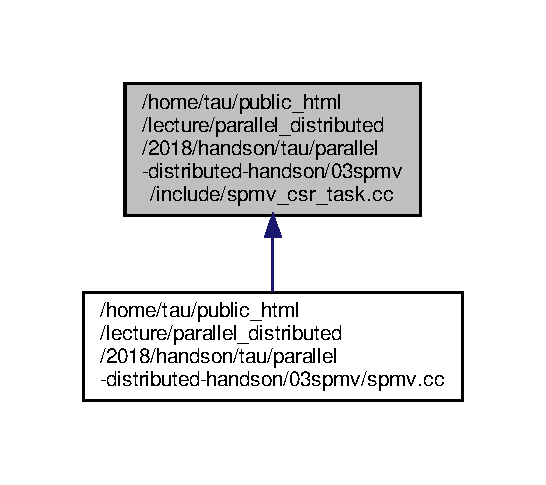
\includegraphics[width=262pt]{spmv__csr__task_8cc__dep__incl}
\end{center}
\end{figure}
\subsection*{Functions}
\begin{DoxyCompactItemize}
\item 
static int \hyperlink{spmv__csr__task_8cc_a3c9bfaecd18fdbead39a82c8b703efa8}{spmv\+\_\+csr\+\_\+task} (\hyperlink{structsparse__t}{sparse\+\_\+t} A, \hyperlink{structvec__t}{vec\+\_\+t} vx, \hyperlink{structvec__t}{vec\+\_\+t} vy)
\begin{DoxyCompactList}\small\item\em y = A $\ast$ x for csr with tasks \end{DoxyCompactList}\end{DoxyCompactItemize}


\subsection{Detailed Description}
y = A $\ast$ x for csr with tasks 



\subsection{Function Documentation}
\mbox{\Hypertarget{spmv__csr__task_8cc_a3c9bfaecd18fdbead39a82c8b703efa8}\label{spmv__csr__task_8cc_a3c9bfaecd18fdbead39a82c8b703efa8}} 
\index{spmv\+\_\+csr\+\_\+task.\+cc@{spmv\+\_\+csr\+\_\+task.\+cc}!spmv\+\_\+csr\+\_\+task@{spmv\+\_\+csr\+\_\+task}}
\index{spmv\+\_\+csr\+\_\+task@{spmv\+\_\+csr\+\_\+task}!spmv\+\_\+csr\+\_\+task.\+cc@{spmv\+\_\+csr\+\_\+task.\+cc}}
\subsubsection{\texorpdfstring{spmv\+\_\+csr\+\_\+task()}{spmv\_csr\_task()}}
{\footnotesize\ttfamily static int spmv\+\_\+csr\+\_\+task (\begin{DoxyParamCaption}\item[{\hyperlink{structsparse__t}{sparse\+\_\+t}}]{A,  }\item[{\hyperlink{structvec__t}{vec\+\_\+t}}]{vx,  }\item[{\hyperlink{structvec__t}{vec\+\_\+t}}]{vy }\end{DoxyParamCaption})\hspace{0.3cm}{\ttfamily [static]}}



y = A $\ast$ x for csr with tasks 


\begin{DoxyParams}{Parameters}
{\em (\+A)} & a sparse matrix \\
\hline
{\em (vx)} & a vector \\
\hline
{\em (vy)} & a vector \\
\hline
\end{DoxyParams}
\begin{DoxyReturn}{Returns}
1 if succeed, 0 if failed 
\end{DoxyReturn}

\hypertarget{spmv__csr__udr_8cc}{}\section{/home/tau/public\+\_\+html/lecture/parallel\+\_\+distributed/2018/handson/tau/parallel-\/distributed-\/handson/03spmv/include/spmv\+\_\+csr\+\_\+udr.cc File Reference}
\label{spmv__csr__udr_8cc}\index{/home/tau/public\+\_\+html/lecture/parallel\+\_\+distributed/2018/handson/tau/parallel-\/distributed-\/handson/03spmv/include/spmv\+\_\+csr\+\_\+udr.\+cc@{/home/tau/public\+\_\+html/lecture/parallel\+\_\+distributed/2018/handson/tau/parallel-\/distributed-\/handson/03spmv/include/spmv\+\_\+csr\+\_\+udr.\+cc}}


y = A $\ast$ x for csr with parallel for + user-\/defined functions  


This graph shows which files directly or indirectly include this file\+:\nopagebreak
\begin{figure}[H]
\begin{center}
\leavevmode
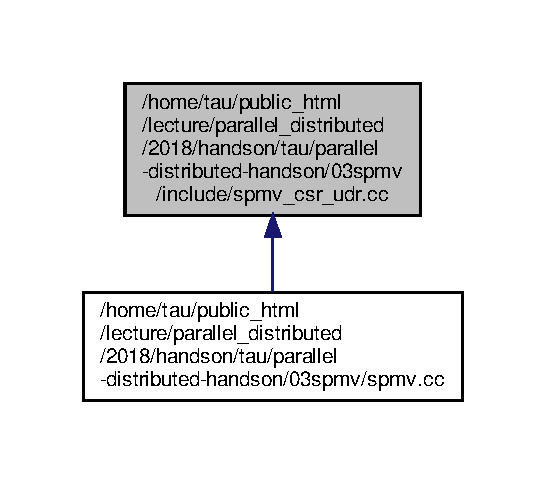
\includegraphics[width=262pt]{spmv__csr__udr_8cc__dep__incl}
\end{center}
\end{figure}
\subsection*{Functions}
\begin{DoxyCompactItemize}
\item 
static int \hyperlink{spmv__csr__udr_8cc_a9bee2a521f90ab82984586d212f437d3}{spmv\+\_\+csr\+\_\+udr} (\hyperlink{structsparse__t}{sparse\+\_\+t} A, \hyperlink{structvec__t}{vec\+\_\+t} vx, \hyperlink{structvec__t}{vec\+\_\+t} vy)
\begin{DoxyCompactList}\small\item\em y = A $\ast$ x for csr with parallel for + user-\/defined functions \end{DoxyCompactList}\end{DoxyCompactItemize}


\subsection{Detailed Description}
y = A $\ast$ x for csr with parallel for + user-\/defined functions 



\subsection{Function Documentation}
\mbox{\Hypertarget{spmv__csr__udr_8cc_a9bee2a521f90ab82984586d212f437d3}\label{spmv__csr__udr_8cc_a9bee2a521f90ab82984586d212f437d3}} 
\index{spmv\+\_\+csr\+\_\+udr.\+cc@{spmv\+\_\+csr\+\_\+udr.\+cc}!spmv\+\_\+csr\+\_\+udr@{spmv\+\_\+csr\+\_\+udr}}
\index{spmv\+\_\+csr\+\_\+udr@{spmv\+\_\+csr\+\_\+udr}!spmv\+\_\+csr\+\_\+udr.\+cc@{spmv\+\_\+csr\+\_\+udr.\+cc}}
\subsubsection{\texorpdfstring{spmv\+\_\+csr\+\_\+udr()}{spmv\_csr\_udr()}}
{\footnotesize\ttfamily static int spmv\+\_\+csr\+\_\+udr (\begin{DoxyParamCaption}\item[{\hyperlink{structsparse__t}{sparse\+\_\+t}}]{A,  }\item[{\hyperlink{structvec__t}{vec\+\_\+t}}]{vx,  }\item[{\hyperlink{structvec__t}{vec\+\_\+t}}]{vy }\end{DoxyParamCaption})\hspace{0.3cm}{\ttfamily [static]}}



y = A $\ast$ x for csr with parallel for + user-\/defined functions 


\begin{DoxyParams}{Parameters}
{\em (\+A)} & a sparse matrix \\
\hline
{\em (vx)} & a vector \\
\hline
{\em (vy)} & a vector \\
\hline
\end{DoxyParams}
\begin{DoxyReturn}{Returns}
1 if succeed, 0 if failed 
\end{DoxyReturn}

\hypertarget{vec__norm2__cuda_8cc}{}\section{/home/tau/public\+\_\+html/lecture/parallel\+\_\+distributed/2018/handson/tau/parallel-\/distributed-\/handson/03spmv/include/vec\+\_\+norm2\+\_\+cuda.cc File Reference}
\label{vec__norm2__cuda_8cc}\index{/home/tau/public\+\_\+html/lecture/parallel\+\_\+distributed/2018/handson/tau/parallel-\/distributed-\/handson/03spmv/include/vec\+\_\+norm2\+\_\+cuda.\+cc@{/home/tau/public\+\_\+html/lecture/parallel\+\_\+distributed/2018/handson/tau/parallel-\/distributed-\/handson/03spmv/include/vec\+\_\+norm2\+\_\+cuda.\+cc}}


the device procedure to do vec\+\_\+norm2 on the device  


\subsection*{Functions}
\begin{DoxyCompactItemize}
\item 
\+\_\+\+\_\+global\+\_\+\+\_\+ void \hyperlink{vec__norm2__cuda_8cc_afe19da671b9e7b759c966363ebff039c}{vec\+\_\+norm2\+\_\+dev} (\hyperlink{structvec__t}{vec\+\_\+t} v, \hyperlink{spmv_8cc_a11d147c64891830c9e79b3315b1b2e21}{real} $\ast$s)
\begin{DoxyCompactList}\small\item\em the device procedure to do vec\+\_\+norm2 on the device \end{DoxyCompactList}\item 
static \hyperlink{spmv_8cc_a11d147c64891830c9e79b3315b1b2e21}{real} \hyperlink{vec__norm2__cuda_8cc_a7dd3cfc8a09a071082c08d902a4ee7bc}{vec\+\_\+norm2\+\_\+cuda} (\hyperlink{structvec__t}{vec\+\_\+t} v)
\begin{DoxyCompactList}\small\item\em square norm of a vector in parallel with cuda \end{DoxyCompactList}\end{DoxyCompactItemize}


\subsection{Detailed Description}
the device procedure to do vec\+\_\+norm2 on the device 



\subsection{Function Documentation}
\mbox{\Hypertarget{vec__norm2__cuda_8cc_a7dd3cfc8a09a071082c08d902a4ee7bc}\label{vec__norm2__cuda_8cc_a7dd3cfc8a09a071082c08d902a4ee7bc}} 
\index{vec\+\_\+norm2\+\_\+cuda.\+cc@{vec\+\_\+norm2\+\_\+cuda.\+cc}!vec\+\_\+norm2\+\_\+cuda@{vec\+\_\+norm2\+\_\+cuda}}
\index{vec\+\_\+norm2\+\_\+cuda@{vec\+\_\+norm2\+\_\+cuda}!vec\+\_\+norm2\+\_\+cuda.\+cc@{vec\+\_\+norm2\+\_\+cuda.\+cc}}
\subsubsection{\texorpdfstring{vec\+\_\+norm2\+\_\+cuda()}{vec\_norm2\_cuda()}}
{\footnotesize\ttfamily static \hyperlink{spmv_8cc_a11d147c64891830c9e79b3315b1b2e21}{real} vec\+\_\+norm2\+\_\+cuda (\begin{DoxyParamCaption}\item[{\hyperlink{structvec__t}{vec\+\_\+t}}]{v }\end{DoxyParamCaption})\hspace{0.3cm}{\ttfamily [static]}}



square norm of a vector in parallel with cuda 


\begin{DoxyParams}{Parameters}
{\em (v)} & a vector \\
\hline
\end{DoxyParams}
\begin{DoxyReturn}{Returns}
the square norm of v (v\mbox{[}0\mbox{]}$^\wedge$2 + ... + v\mbox{[}n-\/1\mbox{]}$^\wedge$2) 
\end{DoxyReturn}
\mbox{\Hypertarget{vec__norm2__cuda_8cc_afe19da671b9e7b759c966363ebff039c}\label{vec__norm2__cuda_8cc_afe19da671b9e7b759c966363ebff039c}} 
\index{vec\+\_\+norm2\+\_\+cuda.\+cc@{vec\+\_\+norm2\+\_\+cuda.\+cc}!vec\+\_\+norm2\+\_\+dev@{vec\+\_\+norm2\+\_\+dev}}
\index{vec\+\_\+norm2\+\_\+dev@{vec\+\_\+norm2\+\_\+dev}!vec\+\_\+norm2\+\_\+cuda.\+cc@{vec\+\_\+norm2\+\_\+cuda.\+cc}}
\subsubsection{\texorpdfstring{vec\+\_\+norm2\+\_\+dev()}{vec\_norm2\_dev()}}
{\footnotesize\ttfamily \+\_\+\+\_\+global\+\_\+\+\_\+ void vec\+\_\+norm2\+\_\+dev (\begin{DoxyParamCaption}\item[{\hyperlink{structvec__t}{vec\+\_\+t}}]{v,  }\item[{\hyperlink{spmv_8cc_a11d147c64891830c9e79b3315b1b2e21}{real} $\ast$}]{s }\end{DoxyParamCaption})}



the device procedure to do vec\+\_\+norm2 on the device 


\begin{DoxyParams}{Parameters}
{\em (v)} & a vector \\
\hline
{\em (s)} & a pointer to a device memory to put the result into\\
\hline
\end{DoxyParams}
assume v.\+elems\+\_\+dev already set and s a proper pointer to a device memory 
\hypertarget{vec__norm2__parallel_8cc}{}\section{/home/tau/public\+\_\+html/lecture/parallel\+\_\+distributed/2018/handson/tau/parallel-\/distributed-\/handson/03spmv/include/vec\+\_\+norm2\+\_\+parallel.cc File Reference}
\label{vec__norm2__parallel_8cc}\index{/home/tau/public\+\_\+html/lecture/parallel\+\_\+distributed/2018/handson/tau/parallel-\/distributed-\/handson/03spmv/include/vec\+\_\+norm2\+\_\+parallel.\+cc@{/home/tau/public\+\_\+html/lecture/parallel\+\_\+distributed/2018/handson/tau/parallel-\/distributed-\/handson/03spmv/include/vec\+\_\+norm2\+\_\+parallel.\+cc}}


square norm of a vector in serial  


This graph shows which files directly or indirectly include this file\+:\nopagebreak
\begin{figure}[H]
\begin{center}
\leavevmode
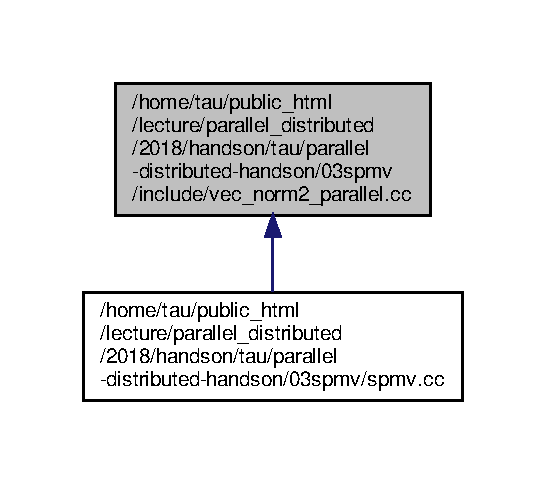
\includegraphics[width=262pt]{vec__norm2__parallel_8cc__dep__incl}
\end{center}
\end{figure}
\subsection*{Functions}
\begin{DoxyCompactItemize}
\item 
static \hyperlink{spmv_8cc_a11d147c64891830c9e79b3315b1b2e21}{real} \hyperlink{vec__norm2__parallel_8cc_a93ea4592e149a2ef18aea41dce0f1cbb}{vec\+\_\+norm2\+\_\+parallel} (\hyperlink{structvec__t}{vec\+\_\+t} v)
\begin{DoxyCompactList}\small\item\em square norm of a vector in serial \end{DoxyCompactList}\end{DoxyCompactItemize}


\subsection{Detailed Description}
square norm of a vector in serial 



\subsection{Function Documentation}
\mbox{\Hypertarget{vec__norm2__parallel_8cc_a93ea4592e149a2ef18aea41dce0f1cbb}\label{vec__norm2__parallel_8cc_a93ea4592e149a2ef18aea41dce0f1cbb}} 
\index{vec\+\_\+norm2\+\_\+parallel.\+cc@{vec\+\_\+norm2\+\_\+parallel.\+cc}!vec\+\_\+norm2\+\_\+parallel@{vec\+\_\+norm2\+\_\+parallel}}
\index{vec\+\_\+norm2\+\_\+parallel@{vec\+\_\+norm2\+\_\+parallel}!vec\+\_\+norm2\+\_\+parallel.\+cc@{vec\+\_\+norm2\+\_\+parallel.\+cc}}
\subsubsection{\texorpdfstring{vec\+\_\+norm2\+\_\+parallel()}{vec\_norm2\_parallel()}}
{\footnotesize\ttfamily static \hyperlink{spmv_8cc_a11d147c64891830c9e79b3315b1b2e21}{real} vec\+\_\+norm2\+\_\+parallel (\begin{DoxyParamCaption}\item[{\hyperlink{structvec__t}{vec\+\_\+t}}]{v }\end{DoxyParamCaption})\hspace{0.3cm}{\ttfamily [static]}}



square norm of a vector in serial 


\begin{DoxyParams}{Parameters}
{\em (v)} & a vector \\
\hline
\end{DoxyParams}
\begin{DoxyReturn}{Returns}
the square norm of v (v\mbox{[}0\mbox{]}$^\wedge$2 + ... + v\mbox{[}n-\/1\mbox{]}$^\wedge$2) 
\end{DoxyReturn}

\hypertarget{vec__norm2__task_8cc}{}\section{/home/tau/public\+\_\+html/lecture/parallel\+\_\+distributed/2018/handson/tau/parallel-\/distributed-\/handson/03spmv/include/vec\+\_\+norm2\+\_\+task.cc File Reference}
\label{vec__norm2__task_8cc}\index{/home/tau/public\+\_\+html/lecture/parallel\+\_\+distributed/2018/handson/tau/parallel-\/distributed-\/handson/03spmv/include/vec\+\_\+norm2\+\_\+task.\+cc@{/home/tau/public\+\_\+html/lecture/parallel\+\_\+distributed/2018/handson/tau/parallel-\/distributed-\/handson/03spmv/include/vec\+\_\+norm2\+\_\+task.\+cc}}


square norm of a vector in serial  


This graph shows which files directly or indirectly include this file\+:\nopagebreak
\begin{figure}[H]
\begin{center}
\leavevmode
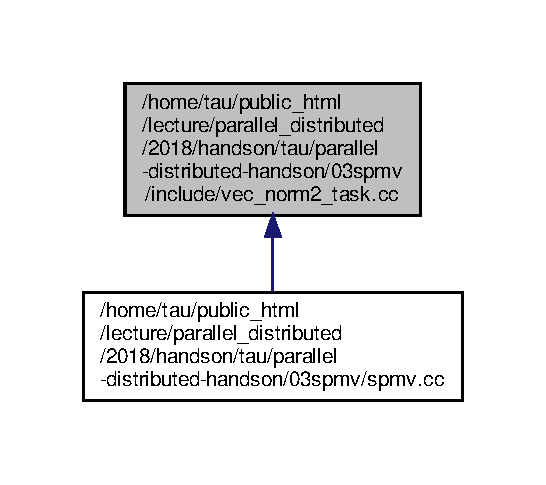
\includegraphics[width=262pt]{vec__norm2__task_8cc__dep__incl}
\end{center}
\end{figure}
\subsection*{Functions}
\begin{DoxyCompactItemize}
\item 
static \hyperlink{spmv_8cc_a11d147c64891830c9e79b3315b1b2e21}{real} \hyperlink{vec__norm2__task_8cc_a66ae15550f3329b3c276dead7d8b7ffc}{vec\+\_\+norm2\+\_\+task} (\hyperlink{structvec__t}{vec\+\_\+t} v)
\begin{DoxyCompactList}\small\item\em square norm of a vector in serial \end{DoxyCompactList}\end{DoxyCompactItemize}


\subsection{Detailed Description}
square norm of a vector in serial 



\subsection{Function Documentation}
\mbox{\Hypertarget{vec__norm2__task_8cc_a66ae15550f3329b3c276dead7d8b7ffc}\label{vec__norm2__task_8cc_a66ae15550f3329b3c276dead7d8b7ffc}} 
\index{vec\+\_\+norm2\+\_\+task.\+cc@{vec\+\_\+norm2\+\_\+task.\+cc}!vec\+\_\+norm2\+\_\+task@{vec\+\_\+norm2\+\_\+task}}
\index{vec\+\_\+norm2\+\_\+task@{vec\+\_\+norm2\+\_\+task}!vec\+\_\+norm2\+\_\+task.\+cc@{vec\+\_\+norm2\+\_\+task.\+cc}}
\subsubsection{\texorpdfstring{vec\+\_\+norm2\+\_\+task()}{vec\_norm2\_task()}}
{\footnotesize\ttfamily static \hyperlink{spmv_8cc_a11d147c64891830c9e79b3315b1b2e21}{real} vec\+\_\+norm2\+\_\+task (\begin{DoxyParamCaption}\item[{\hyperlink{structvec__t}{vec\+\_\+t}}]{v }\end{DoxyParamCaption})\hspace{0.3cm}{\ttfamily [static]}}



square norm of a vector in serial 


\begin{DoxyParams}{Parameters}
{\em (v)} & a vector \\
\hline
\end{DoxyParams}
\begin{DoxyReturn}{Returns}
the square norm of v (v\mbox{[}0\mbox{]}$^\wedge$2 + ... + v\mbox{[}n-\/1\mbox{]}$^\wedge$2) 
\end{DoxyReturn}

\hypertarget{vec__norm2__udr_8cc}{}\section{/home/tau/public\+\_\+html/lecture/parallel\+\_\+distributed/2018/handson/tau/parallel-\/distributed-\/handson/03spmv/include/vec\+\_\+norm2\+\_\+udr.cc File Reference}
\label{vec__norm2__udr_8cc}\index{/home/tau/public\+\_\+html/lecture/parallel\+\_\+distributed/2018/handson/tau/parallel-\/distributed-\/handson/03spmv/include/vec\+\_\+norm2\+\_\+udr.\+cc@{/home/tau/public\+\_\+html/lecture/parallel\+\_\+distributed/2018/handson/tau/parallel-\/distributed-\/handson/03spmv/include/vec\+\_\+norm2\+\_\+udr.\+cc}}


square norm of a vector in parallel using user-\/defined reduction  


This graph shows which files directly or indirectly include this file\+:\nopagebreak
\begin{figure}[H]
\begin{center}
\leavevmode
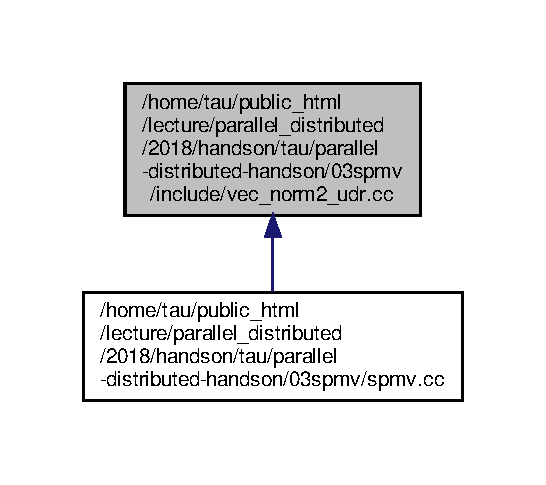
\includegraphics[width=262pt]{vec__norm2__udr_8cc__dep__incl}
\end{center}
\end{figure}
\subsection*{Functions}
\begin{DoxyCompactItemize}
\item 
static \hyperlink{spmv_8cc_a11d147c64891830c9e79b3315b1b2e21}{real} \hyperlink{vec__norm2__udr_8cc_a7559fa49346e732e2002df9c70512d6a}{vec\+\_\+norm2\+\_\+udr} (\hyperlink{structvec__t}{vec\+\_\+t} v)
\begin{DoxyCompactList}\small\item\em square norm of a vector in parallel using user-\/defined reduction \end{DoxyCompactList}\end{DoxyCompactItemize}


\subsection{Detailed Description}
square norm of a vector in parallel using user-\/defined reduction 



\subsection{Function Documentation}
\mbox{\Hypertarget{vec__norm2__udr_8cc_a7559fa49346e732e2002df9c70512d6a}\label{vec__norm2__udr_8cc_a7559fa49346e732e2002df9c70512d6a}} 
\index{vec\+\_\+norm2\+\_\+udr.\+cc@{vec\+\_\+norm2\+\_\+udr.\+cc}!vec\+\_\+norm2\+\_\+udr@{vec\+\_\+norm2\+\_\+udr}}
\index{vec\+\_\+norm2\+\_\+udr@{vec\+\_\+norm2\+\_\+udr}!vec\+\_\+norm2\+\_\+udr.\+cc@{vec\+\_\+norm2\+\_\+udr.\+cc}}
\subsubsection{\texorpdfstring{vec\+\_\+norm2\+\_\+udr()}{vec\_norm2\_udr()}}
{\footnotesize\ttfamily static \hyperlink{spmv_8cc_a11d147c64891830c9e79b3315b1b2e21}{real} vec\+\_\+norm2\+\_\+udr (\begin{DoxyParamCaption}\item[{\hyperlink{structvec__t}{vec\+\_\+t}}]{v }\end{DoxyParamCaption})\hspace{0.3cm}{\ttfamily [static]}}



square norm of a vector in parallel using user-\/defined reduction 


\begin{DoxyParams}{Parameters}
{\em (v)} & a vector \\
\hline
\end{DoxyParams}
\begin{DoxyReturn}{Returns}
the square norm of v (v\mbox{[}0\mbox{]}$^\wedge$2 + ... + v\mbox{[}n-\/1\mbox{]}$^\wedge$2) 
\end{DoxyReturn}

\hypertarget{vec__to__dev_8cc}{}\section{/home/tau/public\+\_\+html/lecture/parallel\+\_\+distributed/2018/handson/tau/parallel-\/distributed-\/handson/03spmv/include/vec\+\_\+to\+\_\+dev.cc File Reference}
\label{vec__to__dev_8cc}\index{/home/tau/public\+\_\+html/lecture/parallel\+\_\+distributed/2018/handson/tau/parallel-\/distributed-\/handson/03spmv/include/vec\+\_\+to\+\_\+dev.\+cc@{/home/tau/public\+\_\+html/lecture/parallel\+\_\+distributed/2018/handson/tau/parallel-\/distributed-\/handson/03spmv/include/vec\+\_\+to\+\_\+dev.\+cc}}


make a deivce copy of a vector.  


\subsection*{Functions}
\begin{DoxyCompactItemize}
\item 
static int \hyperlink{vec__to__dev_8cc_a526773beced925dd5db091a60d74fdcf}{vec\+\_\+to\+\_\+dev} (\hyperlink{structvec__t}{vec\+\_\+t} \&v)
\begin{DoxyCompactList}\small\item\em make a deivce copy of a vector. \end{DoxyCompactList}\end{DoxyCompactItemize}


\subsection{Detailed Description}
make a deivce copy of a vector. 



\subsection{Function Documentation}
\mbox{\Hypertarget{vec__to__dev_8cc_a526773beced925dd5db091a60d74fdcf}\label{vec__to__dev_8cc_a526773beced925dd5db091a60d74fdcf}} 
\index{vec\+\_\+to\+\_\+dev.\+cc@{vec\+\_\+to\+\_\+dev.\+cc}!vec\+\_\+to\+\_\+dev@{vec\+\_\+to\+\_\+dev}}
\index{vec\+\_\+to\+\_\+dev@{vec\+\_\+to\+\_\+dev}!vec\+\_\+to\+\_\+dev.\+cc@{vec\+\_\+to\+\_\+dev.\+cc}}
\subsubsection{\texorpdfstring{vec\+\_\+to\+\_\+dev()}{vec\_to\_dev()}}
{\footnotesize\ttfamily static int vec\+\_\+to\+\_\+dev (\begin{DoxyParamCaption}\item[{\hyperlink{structvec__t}{vec\+\_\+t} \&}]{v }\end{DoxyParamCaption})\hspace{0.3cm}{\ttfamily [static]}}



make a deivce copy of a vector. 


\begin{DoxyParams}{Parameters}
{\em (v)} & the reference to a matrix whose elems\+\_\+dev has not been set (i.\+e., = N\+U\+LL) \\
\hline
\end{DoxyParams}
\begin{DoxyReturn}{Returns}
1 if succeed. 0 if failed. 
\end{DoxyReturn}
\begin{DoxySeeAlso}{See also}
sparse\+\_\+to\+\_\+dev 
\end{DoxySeeAlso}

\hypertarget{spmv_8cc}{}\section{/home/tau/public\+\_\+html/lecture/parallel\+\_\+distributed/2018/handson/tau/parallel-\/distributed-\/handson/03spmv/spmv.cc File Reference}
\label{spmv_8cc}\index{/home/tau/public\+\_\+html/lecture/parallel\+\_\+distributed/2018/handson/tau/parallel-\/distributed-\/handson/03spmv/spmv.\+cc@{/home/tau/public\+\_\+html/lecture/parallel\+\_\+distributed/2018/handson/tau/parallel-\/distributed-\/handson/03spmv/spmv.\+cc}}


sparse matrix vector multiplication  


{\ttfamily \#include $<$assert.\+h$>$}\newline
{\ttfamily \#include $<$math.\+h$>$}\newline
{\ttfamily \#include $<$stdio.\+h$>$}\newline
{\ttfamily \#include $<$stdlib.\+h$>$}\newline
{\ttfamily \#include $<$string.\+h$>$}\newline
{\ttfamily \#include $<$getopt.\+h$>$}\newline
{\ttfamily \#include $<$time.\+h$>$}\newline
{\ttfamily \#include \char`\"{}include/spmv\+\_\+coo\+\_\+parallel.\+cc\char`\"{}}\newline
{\ttfamily \#include \char`\"{}include/spmv\+\_\+coo\+\_\+task.\+cc\char`\"{}}\newline
{\ttfamily \#include \char`\"{}include/spmv\+\_\+coo\+\_\+udr.\+cc\char`\"{}}\newline
{\ttfamily \#include \char`\"{}include/spmv\+\_\+coo\+\_\+sorted\+\_\+parallel.\+cc\char`\"{}}\newline
{\ttfamily \#include \char`\"{}include/spmv\+\_\+coo\+\_\+sorted\+\_\+task.\+cc\char`\"{}}\newline
{\ttfamily \#include \char`\"{}include/spmv\+\_\+coo\+\_\+sorted\+\_\+udr.\+cc\char`\"{}}\newline
{\ttfamily \#include \char`\"{}include/spmv\+\_\+csr\+\_\+parallel.\+cc\char`\"{}}\newline
{\ttfamily \#include \char`\"{}include/spmv\+\_\+csr\+\_\+task.\+cc\char`\"{}}\newline
{\ttfamily \#include \char`\"{}include/spmv\+\_\+csr\+\_\+udr.\+cc\char`\"{}}\newline
{\ttfamily \#include \char`\"{}include/vec\+\_\+norm2\+\_\+parallel.\+cc\char`\"{}}\newline
{\ttfamily \#include \char`\"{}include/vec\+\_\+norm2\+\_\+task.\+cc\char`\"{}}\newline
{\ttfamily \#include \char`\"{}include/vec\+\_\+norm2\+\_\+udr.\+cc\char`\"{}}\newline
{\ttfamily \#include \char`\"{}include/scalar\+\_\+vec\+\_\+parallel.\+cc\char`\"{}}\newline
{\ttfamily \#include \char`\"{}include/scalar\+\_\+vec\+\_\+task.\+cc\char`\"{}}\newline
{\ttfamily \#include \char`\"{}include/scalar\+\_\+vec\+\_\+udr.\+cc\char`\"{}}\newline
Include dependency graph for spmv.\+cc\+:\nopagebreak
\begin{figure}[H]
\begin{center}
\leavevmode
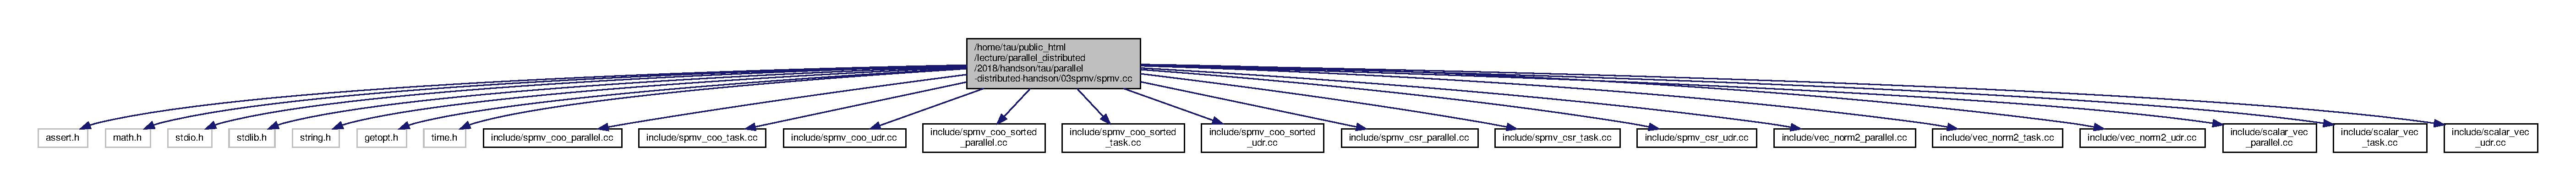
\includegraphics[width=350pt]{spmv_8cc__incl}
\end{center}
\end{figure}
\subsection*{Classes}
\begin{DoxyCompactItemize}
\item 
struct \hyperlink{structcoo__elem__t}{coo\+\_\+elem\+\_\+t}
\begin{DoxyCompactList}\small\item\em an element of coordinate list (i, j, a) \end{DoxyCompactList}\item 
struct \hyperlink{structcsr__elem__t}{csr\+\_\+elem\+\_\+t}
\begin{DoxyCompactList}\small\item\em an element of compressed sparse row \end{DoxyCompactList}\item 
struct \hyperlink{structcoo__t}{coo\+\_\+t}
\begin{DoxyCompactList}\small\item\em sparse matrix in coodinate list format \end{DoxyCompactList}\item 
struct \hyperlink{structcsr__t}{csr\+\_\+t}
\begin{DoxyCompactList}\small\item\em sparse matrix in compressed row format \end{DoxyCompactList}\item 
struct \hyperlink{structsparse__t}{sparse\+\_\+t}
\begin{DoxyCompactList}\small\item\em sparse matrix (in any format) \end{DoxyCompactList}\item 
struct \hyperlink{structvec__t}{vec\+\_\+t}
\begin{DoxyCompactList}\small\item\em vector \end{DoxyCompactList}\item 
struct \hyperlink{structcmdline__options__t}{cmdline\+\_\+options\+\_\+t}
\begin{DoxyCompactList}\small\item\em command line option \end{DoxyCompactList}\item 
struct \hyperlink{structsparse__format__table__entry__t}{sparse\+\_\+format\+\_\+table\+\_\+entry\+\_\+t}
\begin{DoxyCompactList}\small\item\em pair of the index value (sparse\+\_\+format\+\_\+t) and its name \end{DoxyCompactList}\item 
struct \hyperlink{structsparse__format__table__t}{sparse\+\_\+format\+\_\+table\+\_\+t}
\begin{DoxyCompactList}\small\item\em table of sparse format and their names \end{DoxyCompactList}\item 
struct \hyperlink{structsparse__matrix__type__table__entry__t}{sparse\+\_\+matrix\+\_\+type\+\_\+table\+\_\+entry\+\_\+t}
\begin{DoxyCompactList}\small\item\em pair of the index value (matrix\+\_\+type\+\_\+t) and its name \end{DoxyCompactList}\item 
struct \hyperlink{structsparse__matrix__type__table__t}{sparse\+\_\+matrix\+\_\+type\+\_\+table\+\_\+t}
\begin{DoxyCompactList}\small\item\em table of sparse matrix types and their names \end{DoxyCompactList}\item 
struct \hyperlink{structspmv__algo__table__entry__t}{spmv\+\_\+algo\+\_\+table\+\_\+entry\+\_\+t}
\begin{DoxyCompactList}\small\item\em pair of the index value (spmv\+\_\+algo\+\_\+t) and its name \end{DoxyCompactList}\item 
struct \hyperlink{structspmv__algo__table__t}{spmv\+\_\+algo\+\_\+table\+\_\+t}
\begin{DoxyCompactList}\small\item\em table of spmv algorithms and their names \end{DoxyCompactList}\item 
struct \hyperlink{structidx__pair__t}{idx\+\_\+pair\+\_\+t}
\begin{DoxyCompactList}\small\item\em a pair of two indices (i and j) \end{DoxyCompactList}\end{DoxyCompactItemize}
\subsection*{Typedefs}
\begin{DoxyCompactItemize}
\item 
typedef int \hyperlink{spmv_8cc_a8e93478a00e685bea5e6a3f617bf03a3}{idx\+\_\+t}
\begin{DoxyCompactList}\small\item\em type of matrix index (i,j,...) \end{DoxyCompactList}\item 
\mbox{\Hypertarget{spmv_8cc_a11d147c64891830c9e79b3315b1b2e21}\label{spmv_8cc_a11d147c64891830c9e79b3315b1b2e21}} 
typedef double \hyperlink{spmv_8cc_a11d147c64891830c9e79b3315b1b2e21}{real}
\begin{DoxyCompactList}\small\item\em type of a matrix element \end{DoxyCompactList}\end{DoxyCompactItemize}
\subsection*{Enumerations}
\begin{DoxyCompactItemize}
\item 
enum \hyperlink{spmv_8cc_a8c0094893526c01b430903b2d9227256}{sparse\+\_\+format\+\_\+t} \{ \hyperlink{spmv_8cc_a8c0094893526c01b430903b2d9227256a3873dfc9b4303f69130d325bb9d5d3d9}{sparse\+\_\+format\+\_\+coo}, 
\hyperlink{spmv_8cc_a8c0094893526c01b430903b2d9227256ae622b3c6575c5efae6930339af50e076}{sparse\+\_\+format\+\_\+coo\+\_\+sorted}, 
\hyperlink{spmv_8cc_a8c0094893526c01b430903b2d9227256a8d3a61cb0ac76c8b5334c24c7618c4c7}{sparse\+\_\+format\+\_\+csr}, 
\hyperlink{spmv_8cc_a8c0094893526c01b430903b2d9227256adc326179d0d559f82edc8cd35be11de5}{sparse\+\_\+format\+\_\+invalid}
 \}\begin{DoxyCompactList}\small\item\em sparse matrix storage format \end{DoxyCompactList}
\item 
enum \hyperlink{spmv_8cc_a43a568fb26bc32aeaad07769cc524c45}{sparse\+\_\+matrix\+\_\+type\+\_\+t} \{ \newline
\hyperlink{spmv_8cc_a43a568fb26bc32aeaad07769cc524c45a7d1a4297606841df02daaf788b3c747e}{sparse\+\_\+matrix\+\_\+type\+\_\+random}, 
\hyperlink{spmv_8cc_a43a568fb26bc32aeaad07769cc524c45ad678d1380d3392961348a30105bfa5ae}{sparse\+\_\+matrix\+\_\+type\+\_\+rmat}, 
\hyperlink{spmv_8cc_a43a568fb26bc32aeaad07769cc524c45a279601049abdf78851fca2cd657d59fc}{sparse\+\_\+matrix\+\_\+type\+\_\+one}, 
\hyperlink{spmv_8cc_a43a568fb26bc32aeaad07769cc524c45a86751f08b859e672050ab331cc3aefd6}{sparse\+\_\+matrix\+\_\+type\+\_\+coo\+\_\+file}, 
\newline
\hyperlink{spmv_8cc_a43a568fb26bc32aeaad07769cc524c45adbd59ebb0cfb220b9035a64fc2ed28dc}{sparse\+\_\+matrix\+\_\+type\+\_\+invalid}
 \}\begin{DoxyCompactList}\small\item\em type of sparse matrix we work on (how to generate elements) \end{DoxyCompactList}
\item 
enum \hyperlink{spmv_8cc_ad2cf0493af54bf76c5be68b4634fcab7}{spmv\+\_\+algo\+\_\+t} \{ \newline
\hyperlink{spmv_8cc_ad2cf0493af54bf76c5be68b4634fcab7a8239a128e5970e7f36aec71d6265d78a}{spmv\+\_\+algo\+\_\+serial}, 
\hyperlink{spmv_8cc_ad2cf0493af54bf76c5be68b4634fcab7abbdcd58ce962bc8134af08a7f4310f81}{spmv\+\_\+algo\+\_\+parallel}, 
\hyperlink{spmv_8cc_ad2cf0493af54bf76c5be68b4634fcab7a1f9366271f2cabad112a5a32d3c25b09}{spmv\+\_\+algo\+\_\+cuda}, 
\hyperlink{spmv_8cc_ad2cf0493af54bf76c5be68b4634fcab7abf06dbea21c647da540099ac2b982c7c}{spmv\+\_\+algo\+\_\+task}, 
\newline
\hyperlink{spmv_8cc_ad2cf0493af54bf76c5be68b4634fcab7a874bdd20649b02a010a566b72759db44}{spmv\+\_\+algo\+\_\+udr}, 
\hyperlink{spmv_8cc_ad2cf0493af54bf76c5be68b4634fcab7add2a1e0329d677ee5f5fcc7ee8077dd0}{spmv\+\_\+algo\+\_\+invalid}
 \}\begin{DoxyCompactList}\small\item\em spmv matrix algorithm \end{DoxyCompactList}
\end{DoxyCompactItemize}
\subsection*{Functions}
\begin{DoxyCompactItemize}
\item 
static long \hyperlink{spmv_8cc_ae8a11dfbc1a073b8ea09b2b25484df8e}{cur\+\_\+time\+\_\+ns} ()
\begin{DoxyCompactList}\small\item\em current time in nano second \end{DoxyCompactList}\item 
static void $\ast$ \hyperlink{spmv_8cc_a3cab6fa93276c69712c867ea0c9480c9}{xalloc} (size\+\_\+t sz)
\begin{DoxyCompactList}\small\item\em malloc + check \end{DoxyCompactList}\item 
static void \hyperlink{spmv_8cc_ab74147af88fbc62f9076539683737f69}{xfree} (void $\ast$a)
\begin{DoxyCompactList}\small\item\em wrap free \end{DoxyCompactList}\item 
\mbox{\Hypertarget{spmv_8cc_a9d14968d7ef360d5dc0f32527754de79}\label{spmv_8cc_a9d14968d7ef360d5dc0f32527754de79}} 
static \hyperlink{structcmdline__options__t}{cmdline\+\_\+options\+\_\+t} \hyperlink{spmv_8cc_a9d14968d7ef360d5dc0f32527754de79}{default\+\_\+opts} ()
\begin{DoxyCompactList}\small\item\em default values for command line options \end{DoxyCompactList}\item 
\mbox{\Hypertarget{spmv_8cc_ae06a8b4681f9cd8d90bee9de540a0d13}\label{spmv_8cc_ae06a8b4681f9cd8d90bee9de540a0d13}} 
static char $\ast$ \hyperlink{spmv_8cc_ae06a8b4681f9cd8d90bee9de540a0d13}{sparse\+\_\+format\+\_\+strs} ()
\begin{DoxyCompactList}\small\item\em a comma-\/separated list of available sparse formats \end{DoxyCompactList}\item 
\mbox{\Hypertarget{spmv_8cc_a5aeee7bb92b870eab6ebc6a6ad55228e}\label{spmv_8cc_a5aeee7bb92b870eab6ebc6a6ad55228e}} 
static char $\ast$ \hyperlink{spmv_8cc_a5aeee7bb92b870eab6ebc6a6ad55228e}{sparse\+\_\+matrix\+\_\+type\+\_\+strs} ()
\begin{DoxyCompactList}\small\item\em a comma-\/separated list of available matrix types \end{DoxyCompactList}\item 
\mbox{\Hypertarget{spmv_8cc_af6ccf5c32cd788e8a8f0a04b25996b32}\label{spmv_8cc_af6ccf5c32cd788e8a8f0a04b25996b32}} 
static char $\ast$ \hyperlink{spmv_8cc_af6ccf5c32cd788e8a8f0a04b25996b32}{spmv\+\_\+algo\+\_\+strs} ()
\begin{DoxyCompactList}\small\item\em print a comma-\/separated list of available algorithms to the standard error \end{DoxyCompactList}\item 
static void \hyperlink{spmv_8cc_adf81d1a5d4b0a2db9fcf090141069e7c}{cmdline\+\_\+options\+\_\+destroy} (\hyperlink{structcmdline__options__t}{cmdline\+\_\+options\+\_\+t} opt)
\begin{DoxyCompactList}\small\item\em release memory for cmdline\+\_\+options \end{DoxyCompactList}\item 
static void \hyperlink{spmv_8cc_a848c0ca46d3e3ecc39d2fccc4d85fa12}{usage} (const char $\ast$prog)
\begin{DoxyCompactList}\small\item\em print usage \end{DoxyCompactList}\item 
static \hyperlink{spmv_8cc_a8c0094893526c01b430903b2d9227256}{sparse\+\_\+format\+\_\+t} \hyperlink{spmv_8cc_a3363fba87122e57b925704a8394f405d}{parse\+\_\+sparse\+\_\+format} (char $\ast$s)
\begin{DoxyCompactList}\small\item\em parse a string for matrix format and return an enum value \end{DoxyCompactList}\item 
static \hyperlink{spmv_8cc_a43a568fb26bc32aeaad07769cc524c45}{sparse\+\_\+matrix\+\_\+type\+\_\+t} \hyperlink{spmv_8cc_a7975e4e4d7080a5380dba1a9d11b3d99}{parse\+\_\+sparse\+\_\+matrix\+\_\+type} (char $\ast$s)
\begin{DoxyCompactList}\small\item\em parse a string for sparse matrix type and return an enum value \end{DoxyCompactList}\item 
static \hyperlink{spmv_8cc_ad2cf0493af54bf76c5be68b4634fcab7}{spmv\+\_\+algo\+\_\+t} \hyperlink{spmv_8cc_a9719a9f5e00e078d0ee1039b890a9f7a}{parse\+\_\+spmv\+\_\+algo} (char $\ast$s)
\begin{DoxyCompactList}\small\item\em parse a string for spmv algorithm and return an enum value \end{DoxyCompactList}\item 
\mbox{\Hypertarget{spmv_8cc_ac20283b7c6670bcd771e99ebbe84dcac}\label{spmv_8cc_ac20283b7c6670bcd771e99ebbe84dcac}} 
static void \hyperlink{spmv_8cc_ac20283b7c6670bcd771e99ebbe84dcac}{parse\+\_\+error\+\_\+rmat\+\_\+probability} (char $\ast$rmat\+\_\+str)
\begin{DoxyCompactList}\small\item\em print error meessage during rmat string (a,b,c,d) \end{DoxyCompactList}\item 
static int \hyperlink{spmv_8cc_a4f85d868c74dc8293760c01c26699663}{parse\+\_\+rmat\+\_\+probability} (char $\ast$rmat\+\_\+str, double rmat\mbox{[}2\mbox{]}\mbox{[}2\mbox{]})
\begin{DoxyCompactList}\small\item\em parse a string of the form a,b,c,d and put it into 2x2 matrix \end{DoxyCompactList}\item 
static \hyperlink{structcmdline__options__t}{cmdline\+\_\+options\+\_\+t} \hyperlink{spmv_8cc_a2564bee68cf55b040dde9891e850fd60}{parse\+\_\+args} (int argc, char $\ast$$\ast$argv)
\begin{DoxyCompactList}\small\item\em parse command line args \end{DoxyCompactList}\item 
\mbox{\Hypertarget{spmv_8cc_a722d5677632ee1f02e98ddbd8a5be12c}\label{spmv_8cc_a722d5677632ee1f02e98ddbd8a5be12c}} 
static \hyperlink{structsparse__t}{sparse\+\_\+t} \hyperlink{spmv_8cc_a722d5677632ee1f02e98ddbd8a5be12c}{mk\+\_\+sparse\+\_\+invalid} ()
\begin{DoxyCompactList}\small\item\em make an invalid matrix \end{DoxyCompactList}\item 
\mbox{\Hypertarget{spmv_8cc_a7cd0154a7fd92d751e3db7fad63a11c7}\label{spmv_8cc_a7cd0154a7fd92d751e3db7fad63a11c7}} 
static void \hyperlink{spmv_8cc_a7cd0154a7fd92d751e3db7fad63a11c7}{coo\+\_\+destroy} (\hyperlink{structsparse__t}{sparse\+\_\+t} A)
\begin{DoxyCompactList}\small\item\em destroy coo \end{DoxyCompactList}\item 
\mbox{\Hypertarget{spmv_8cc_a6431a82194d2f65cb5111edbd4b6a80e}\label{spmv_8cc_a6431a82194d2f65cb5111edbd4b6a80e}} 
static void \hyperlink{spmv_8cc_a6431a82194d2f65cb5111edbd4b6a80e}{csr\+\_\+destroy} (\hyperlink{structsparse__t}{sparse\+\_\+t} A)
\begin{DoxyCompactList}\small\item\em destroy csr \end{DoxyCompactList}\item 
\mbox{\Hypertarget{spmv_8cc_a0572abe0596fb337714fec7fb9a264fd}\label{spmv_8cc_a0572abe0596fb337714fec7fb9a264fd}} 
static void \hyperlink{spmv_8cc_a0572abe0596fb337714fec7fb9a264fd}{sparse\+\_\+destroy} (\hyperlink{structsparse__t}{sparse\+\_\+t} A)
\begin{DoxyCompactList}\small\item\em destroy sparse matrix in any format \end{DoxyCompactList}\item 
\mbox{\Hypertarget{spmv_8cc_a8ce914cc82d0a77c7c53c1e1fd3afe0d}\label{spmv_8cc_a8ce914cc82d0a77c7c53c1e1fd3afe0d}} 
static void \hyperlink{spmv_8cc_a8ce914cc82d0a77c7c53c1e1fd3afe0d}{vec\+\_\+destroy} (\hyperlink{structvec__t}{vec\+\_\+t} x)
\begin{DoxyCompactList}\small\item\em destroy vector \end{DoxyCompactList}\item 
static \hyperlink{structsparse__t}{sparse\+\_\+t} \hyperlink{spmv_8cc_a6069ac893592050e619f9077c99f7493}{mk\+\_\+coo\+\_\+random} (\hyperlink{spmv_8cc_a8e93478a00e685bea5e6a3f617bf03a3}{idx\+\_\+t} M, \hyperlink{spmv_8cc_a8e93478a00e685bea5e6a3f617bf03a3}{idx\+\_\+t} N, \hyperlink{spmv_8cc_a8e93478a00e685bea5e6a3f617bf03a3}{idx\+\_\+t} nnz, unsigned short rg\mbox{[}3\mbox{]})
\begin{DoxyCompactList}\small\item\em make a uniform random coo matrix \end{DoxyCompactList}\item 
static \hyperlink{structidx__pair__t}{idx\+\_\+pair\+\_\+t} \hyperlink{spmv_8cc_ae1de2a8faf2f1567e0c4038c3115bef1}{rmat\+\_\+choose\+\_\+01} (double p\mbox{[}2\mbox{]}\mbox{[}2\mbox{]}, unsigned short rg\mbox{[}3\mbox{]})
\begin{DoxyCompactList}\small\item\em choose a pair of 0/1s according to 2x2 probability matrix p\mbox{[}2\mbox{]}\mbox{[}2\mbox{]}. \end{DoxyCompactList}\item 
static \hyperlink{structidx__pair__t}{idx\+\_\+pair\+\_\+t} \hyperlink{spmv_8cc_a9b363aef130851519b0decb6895ad348}{rmat\+\_\+choose\+\_\+pair} (\hyperlink{spmv_8cc_a8e93478a00e685bea5e6a3f617bf03a3}{idx\+\_\+t} M, \hyperlink{spmv_8cc_a8e93478a00e685bea5e6a3f617bf03a3}{idx\+\_\+t} N, double p\mbox{[}2\mbox{]}\mbox{[}2\mbox{]}, unsigned short rg\mbox{[}3\mbox{]})
\begin{DoxyCompactList}\small\item\em choose (i,j) 0 $<$= i $<$ M and 0 $<$= j $<$ N according to the probability p. \end{DoxyCompactList}\item 
static \hyperlink{structsparse__t}{sparse\+\_\+t} \hyperlink{spmv_8cc_a34835dc746f4196b1c9b0f0ab4be68dd}{mk\+\_\+coo\+\_\+rmat} (\hyperlink{spmv_8cc_a8e93478a00e685bea5e6a3f617bf03a3}{idx\+\_\+t} M, \hyperlink{spmv_8cc_a8e93478a00e685bea5e6a3f617bf03a3}{idx\+\_\+t} N, \hyperlink{spmv_8cc_a8e93478a00e685bea5e6a3f617bf03a3}{idx\+\_\+t} nnz, double p\mbox{[}2\mbox{]}\mbox{[}2\mbox{]}, unsigned short rg\mbox{[}3\mbox{]})
\begin{DoxyCompactList}\small\item\em make a random R-\/\+M\+AT (\href{https://epubs.siam.org/doi/abs/10.1137/1.9781611972740.43}{\tt https\+://epubs.\+siam.\+org/doi/abs/10.\+1137/1.\+9781611972740.\+43}) \end{DoxyCompactList}\item 
static \hyperlink{structsparse__t}{sparse\+\_\+t} \hyperlink{spmv_8cc_a47eb7ed66be3bc240e816ba99c2e27d9}{mk\+\_\+coo\+\_\+one} (\hyperlink{spmv_8cc_a8e93478a00e685bea5e6a3f617bf03a3}{idx\+\_\+t} M, \hyperlink{spmv_8cc_a8e93478a00e685bea5e6a3f617bf03a3}{idx\+\_\+t} N, \hyperlink{spmv_8cc_a8e93478a00e685bea5e6a3f617bf03a3}{idx\+\_\+t} nnz)
\begin{DoxyCompactList}\small\item\em make a sparse matrix whose elements are one on certain rows/columns and zero anywhere else \end{DoxyCompactList}\item 
static int \hyperlink{spmv_8cc_abbc6740cae208e212acc9b0d4079aa3d}{coo\+\_\+elem\+\_\+cmp} (const void $\ast$a\+\_\+, const void $\ast$b\+\_\+)
\begin{DoxyCompactList}\small\item\em compare two coo elements \end{DoxyCompactList}\item 
static \hyperlink{structsparse__t}{sparse\+\_\+t} \hyperlink{spmv_8cc_a5775ee274ee21f69a5165960350c53ab}{sparse\+\_\+coo\+\_\+to\+\_\+coo} (\hyperlink{structsparse__t}{sparse\+\_\+t} A, \hyperlink{spmv_8cc_a8c0094893526c01b430903b2d9227256}{sparse\+\_\+format\+\_\+t} format)
\begin{DoxyCompactList}\small\item\em convert coo/coo\+\_\+sorted matrix A to coo/coo\+\_\+sorted format. \end{DoxyCompactList}\item 
static \hyperlink{structsparse__t}{sparse\+\_\+t} \hyperlink{spmv_8cc_a87dcc54785756a1805e23d25d3b6022a}{sparse\+\_\+coo\+\_\+sorted\+\_\+to\+\_\+csr} (\hyperlink{structsparse__t}{sparse\+\_\+t} A)
\begin{DoxyCompactList}\small\item\em convert a sparse matrix in coo format to csr format. \end{DoxyCompactList}\item 
static \hyperlink{structsparse__t}{sparse\+\_\+t} \hyperlink{spmv_8cc_a701914576bbcd3c9520fd42227481f0b}{sparse\+\_\+coo\+\_\+to\+\_\+csr} (\hyperlink{structsparse__t}{sparse\+\_\+t} A)
\begin{DoxyCompactList}\small\item\em convert a sparse matrix in coo format to csr format. \end{DoxyCompactList}\item 
static \hyperlink{structsparse__t}{sparse\+\_\+t} \hyperlink{spmv_8cc_a3b9867ec850b1a529ebc3d829d81bd2e}{sparse\+\_\+coo\+\_\+to\+\_\+any} (\hyperlink{structsparse__t}{sparse\+\_\+t} A, \hyperlink{spmv_8cc_a8c0094893526c01b430903b2d9227256}{sparse\+\_\+format\+\_\+t} format)
\begin{DoxyCompactList}\small\item\em convert sparse matrix in coo format to any specified format. \end{DoxyCompactList}\item 
static \hyperlink{structsparse__t}{sparse\+\_\+t} \hyperlink{spmv_8cc_ac798b76107ea7ecf5b15736bfa0e79bb}{sparse\+\_\+csr\+\_\+to\+\_\+coo\+\_\+sorted} (\hyperlink{structsparse__t}{sparse\+\_\+t} A)
\begin{DoxyCompactList}\small\item\em convert a sparse matrix in csr format to coo sorted format. \end{DoxyCompactList}\item 
static \hyperlink{structsparse__t}{sparse\+\_\+t} \hyperlink{spmv_8cc_a5b6db8fe4111d00253055e79c76cbef2}{sparse\+\_\+csr\+\_\+to\+\_\+any} (\hyperlink{structsparse__t}{sparse\+\_\+t} A, \hyperlink{spmv_8cc_a8c0094893526c01b430903b2d9227256}{sparse\+\_\+format\+\_\+t} format)
\begin{DoxyCompactList}\small\item\em convert sparse matrix in csr format to any specified format \end{DoxyCompactList}\item 
\hyperlink{structsparse__t}{sparse\+\_\+t} \hyperlink{spmv_8cc_a6828f56a352d81ea9008a66ee2d28706}{sparse\+\_\+any\+\_\+to\+\_\+any} (\hyperlink{structsparse__t}{sparse\+\_\+t} A, \hyperlink{spmv_8cc_a8c0094893526c01b430903b2d9227256}{sparse\+\_\+format\+\_\+t} format)
\begin{DoxyCompactList}\small\item\em convert a sparse matrix of any format to any specified format \end{DoxyCompactList}\item 
static \hyperlink{structsparse__t}{sparse\+\_\+t} \hyperlink{spmv_8cc_a699fcadba85b607a7d6f801ec01d1f21}{read\+\_\+coo\+\_\+file} (\hyperlink{spmv_8cc_a8e93478a00e685bea5e6a3f617bf03a3}{idx\+\_\+t} M, \hyperlink{spmv_8cc_a8e93478a00e685bea5e6a3f617bf03a3}{idx\+\_\+t} N, \hyperlink{spmv_8cc_a8e93478a00e685bea5e6a3f617bf03a3}{idx\+\_\+t} nnz, char $\ast$file)
\begin{DoxyCompactList}\small\item\em read a matrix file and return a sparse matrix in coo formated \end{DoxyCompactList}\item 
static \hyperlink{structsparse__t}{sparse\+\_\+t} \hyperlink{spmv_8cc_ac2f5814f1a6cb86bbdc3dc6d99a2f0bb}{mk\+\_\+sparse\+\_\+matrix\+\_\+coo} (\hyperlink{structcmdline__options__t}{cmdline\+\_\+options\+\_\+t} opt, \hyperlink{spmv_8cc_a8e93478a00e685bea5e6a3f617bf03a3}{idx\+\_\+t} M, \hyperlink{spmv_8cc_a8e93478a00e685bea5e6a3f617bf03a3}{idx\+\_\+t} N, \hyperlink{spmv_8cc_a8e93478a00e685bea5e6a3f617bf03a3}{idx\+\_\+t} nnz, unsigned short rg\mbox{[}3\mbox{]})
\begin{DoxyCompactList}\small\item\em make a sparse matrix in coo format by the desiginated generation method \end{DoxyCompactList}\item 
static \hyperlink{structsparse__t}{sparse\+\_\+t} \hyperlink{spmv_8cc_aaaea896bc16745cbe40e0c8f7c8122b6}{mk\+\_\+sparse\+\_\+matrix} (\hyperlink{structcmdline__options__t}{cmdline\+\_\+options\+\_\+t} opt, \hyperlink{spmv_8cc_a8e93478a00e685bea5e6a3f617bf03a3}{idx\+\_\+t} M, \hyperlink{spmv_8cc_a8e93478a00e685bea5e6a3f617bf03a3}{idx\+\_\+t} N, \hyperlink{spmv_8cc_a8e93478a00e685bea5e6a3f617bf03a3}{idx\+\_\+t} nnz, unsigned short rg\mbox{[}3\mbox{]})
\begin{DoxyCompactList}\small\item\em make (read or generate) a sparse matrix with the specified matrix generation method \end{DoxyCompactList}\item 
static \hyperlink{structsparse__t}{sparse\+\_\+t} \hyperlink{spmv_8cc_a8ef55e202b83e585e5680f3321518bd7}{coo\+\_\+transpose} (\hyperlink{structsparse__t}{sparse\+\_\+t} A)
\begin{DoxyCompactList}\small\item\em transpose a matrix in coordinate list format \end{DoxyCompactList}\item 
static \hyperlink{structsparse__t}{sparse\+\_\+t} \hyperlink{spmv_8cc_a2c4e3e9eaa31cfe79eae1706c4f17402}{sparse\+\_\+transpose} (\hyperlink{structsparse__t}{sparse\+\_\+t} A)
\begin{DoxyCompactList}\small\item\em transpose a matrix in any format \end{DoxyCompactList}\item 
static int \hyperlink{spmv_8cc_a412810ce929de396176940d889f65cff}{spmv\+\_\+coo\+\_\+serial} (\hyperlink{structsparse__t}{sparse\+\_\+t} A, \hyperlink{structvec__t}{vec\+\_\+t} vx, \hyperlink{structvec__t}{vec\+\_\+t} vy)
\begin{DoxyCompactList}\small\item\em y = A $\ast$ x in serial for coo format \end{DoxyCompactList}\item 
static int \hyperlink{spmv_8cc_a3e784ac12f70b7ec0aa027afae47fdb2}{spmv\+\_\+coo} (\hyperlink{spmv_8cc_ad2cf0493af54bf76c5be68b4634fcab7}{spmv\+\_\+algo\+\_\+t} algo, \hyperlink{structsparse__t}{sparse\+\_\+t} A, \hyperlink{structvec__t}{vec\+\_\+t} x, \hyperlink{structvec__t}{vec\+\_\+t} y)
\begin{DoxyCompactList}\small\item\em y = A $\ast$ x for coo format, with the specified algorithm \end{DoxyCompactList}\item 
static int \hyperlink{spmv_8cc_a0c6271c89e03dfba15b7d3e8870dc367}{spmv\+\_\+coo\+\_\+sorted\+\_\+serial} (\hyperlink{structsparse__t}{sparse\+\_\+t} A, \hyperlink{structvec__t}{vec\+\_\+t} vx, \hyperlink{structvec__t}{vec\+\_\+t} vy)
\begin{DoxyCompactList}\small\item\em y = A $\ast$ x in serial for coo\+\_\+sorted format \end{DoxyCompactList}\item 
static int \hyperlink{spmv_8cc_a12ff0f51c705a939cfbc88d2a3e57666}{spmv\+\_\+coo\+\_\+sorted} (\hyperlink{spmv_8cc_ad2cf0493af54bf76c5be68b4634fcab7}{spmv\+\_\+algo\+\_\+t} algo, \hyperlink{structsparse__t}{sparse\+\_\+t} A, \hyperlink{structvec__t}{vec\+\_\+t} x, \hyperlink{structvec__t}{vec\+\_\+t} y)
\begin{DoxyCompactList}\small\item\em y = A $\ast$ x for coo\+\_\+sorted format, with the specified algorithm \end{DoxyCompactList}\item 
static int \hyperlink{spmv_8cc_a8ed522b06ef48963006af213f6c31ff0}{spmv\+\_\+csr\+\_\+serial} (\hyperlink{structsparse__t}{sparse\+\_\+t} A, \hyperlink{structvec__t}{vec\+\_\+t} vx, \hyperlink{structvec__t}{vec\+\_\+t} vy)
\begin{DoxyCompactList}\small\item\em y = A $\ast$ x in serial for csr format \end{DoxyCompactList}\item 
static int \hyperlink{spmv_8cc_a1c45a35e7f86149cec61f9378c32f2e4}{spmv\+\_\+csr} (\hyperlink{spmv_8cc_ad2cf0493af54bf76c5be68b4634fcab7}{spmv\+\_\+algo\+\_\+t} algo, \hyperlink{structsparse__t}{sparse\+\_\+t} A, \hyperlink{structvec__t}{vec\+\_\+t} x, \hyperlink{structvec__t}{vec\+\_\+t} y)
\begin{DoxyCompactList}\small\item\em y = A $\ast$ x for csr format, with the specified algorithm \end{DoxyCompactList}\item 
static int \hyperlink{spmv_8cc_a0b17c7c1f5341c44b046f2f96173dbb3}{spmv} (\hyperlink{spmv_8cc_ad2cf0493af54bf76c5be68b4634fcab7}{spmv\+\_\+algo\+\_\+t} algo, \hyperlink{structsparse__t}{sparse\+\_\+t} A, \hyperlink{structvec__t}{vec\+\_\+t} x, \hyperlink{structvec__t}{vec\+\_\+t} y)
\begin{DoxyCompactList}\small\item\em y = A $\ast$ x for any format, with the specified algorithm \end{DoxyCompactList}\item 
static \hyperlink{spmv_8cc_a11d147c64891830c9e79b3315b1b2e21}{real} \hyperlink{spmv_8cc_afa238f5dc75b2607322dc4b8af535033}{vec\+\_\+norm2\+\_\+serial} (\hyperlink{structvec__t}{vec\+\_\+t} v)
\begin{DoxyCompactList}\small\item\em square norm of a vector in serial \end{DoxyCompactList}\item 
static \hyperlink{spmv_8cc_a11d147c64891830c9e79b3315b1b2e21}{real} \hyperlink{spmv_8cc_a821b3dbaf3109c1340408d104a32849d}{vec\+\_\+norm2} (\hyperlink{spmv_8cc_ad2cf0493af54bf76c5be68b4634fcab7}{spmv\+\_\+algo\+\_\+t} algo, \hyperlink{structvec__t}{vec\+\_\+t} v)
\begin{DoxyCompactList}\small\item\em square norm of a vector with the specified algorithm \end{DoxyCompactList}\item 
static int \hyperlink{spmv_8cc_a99456e0344c1c61bd3040fe14b215cba}{scalar\+\_\+vec\+\_\+serial} (\hyperlink{spmv_8cc_a11d147c64891830c9e79b3315b1b2e21}{real} k, \hyperlink{structvec__t}{vec\+\_\+t} v)
\begin{DoxyCompactList}\small\item\em k x v in serial \end{DoxyCompactList}\item 
static int \hyperlink{spmv_8cc_aacc75d6198977fcb25da335869bccb18}{scalar\+\_\+vec} (\hyperlink{spmv_8cc_ad2cf0493af54bf76c5be68b4634fcab7}{spmv\+\_\+algo\+\_\+t} algo, \hyperlink{spmv_8cc_a11d147c64891830c9e79b3315b1b2e21}{real} k, \hyperlink{structvec__t}{vec\+\_\+t} v)
\begin{DoxyCompactList}\small\item\em k x v in parallel with the specified algorithm \end{DoxyCompactList}\item 
static \hyperlink{spmv_8cc_a11d147c64891830c9e79b3315b1b2e21}{real} \hyperlink{spmv_8cc_a241e0fa53a3f51410d20d83e2a3029c0}{vec\+\_\+normalize} (\hyperlink{spmv_8cc_ad2cf0493af54bf76c5be68b4634fcab7}{spmv\+\_\+algo\+\_\+t} algo, \hyperlink{structvec__t}{vec\+\_\+t} v)
\begin{DoxyCompactList}\small\item\em normalize a vector with the specified algortihm \end{DoxyCompactList}\item 
static \hyperlink{spmv_8cc_a11d147c64891830c9e79b3315b1b2e21}{real} \hyperlink{spmv_8cc_a4cd4c7a560d79a951f87fae71f800def}{repeat\+\_\+spmv} (\hyperlink{spmv_8cc_ad2cf0493af54bf76c5be68b4634fcab7}{spmv\+\_\+algo\+\_\+t} algo, \hyperlink{structsparse__t}{sparse\+\_\+t} \&A, \hyperlink{structsparse__t}{sparse\+\_\+t} \&tA, \hyperlink{structvec__t}{vec\+\_\+t} \&x, \hyperlink{structvec__t}{vec\+\_\+t} \&y, \hyperlink{spmv_8cc_a8e93478a00e685bea5e6a3f617bf03a3}{idx\+\_\+t} repeat)
\begin{DoxyCompactList}\small\item\em repeat y = A x; x = tA y; many times, with the specified algorithm \end{DoxyCompactList}\item 
static \hyperlink{structvec__t}{vec\+\_\+t} \hyperlink{spmv_8cc_a47c4281acee355d11976dcd1bdea57a5}{mk\+\_\+vec\+\_\+random} (\hyperlink{spmv_8cc_a8e93478a00e685bea5e6a3f617bf03a3}{idx\+\_\+t} n, unsigned short rg\mbox{[}3\mbox{]})
\begin{DoxyCompactList}\small\item\em make a random vector of n elements \end{DoxyCompactList}\item 
static \hyperlink{structvec__t}{vec\+\_\+t} \hyperlink{spmv_8cc_a11f770f55b8dbdfd51fb5e6c3764f0d7}{mk\+\_\+vec\+\_\+unit\+\_\+random} (\hyperlink{spmv_8cc_a8e93478a00e685bea5e6a3f617bf03a3}{idx\+\_\+t} n, unsigned short rg\mbox{[}3\mbox{]})
\begin{DoxyCompactList}\small\item\em make a random unit-\/length vector of n elements \end{DoxyCompactList}\item 
static \hyperlink{structvec__t}{vec\+\_\+t} \hyperlink{spmv_8cc_ae5980ab044cde4d173d802a048724abe}{mk\+\_\+vec\+\_\+zero} (\hyperlink{spmv_8cc_a8e93478a00e685bea5e6a3f617bf03a3}{idx\+\_\+t} n)
\begin{DoxyCompactList}\small\item\em make a zero vector of n elements \end{DoxyCompactList}\item 
static int \hyperlink{spmv_8cc_a99d82b31b353c22a745c729d4fdeb64b}{cmp\+\_\+idx\+\_\+fun} (const void $\ast$a\+\_\+, const void $\ast$b\+\_\+)
\begin{DoxyCompactList}\small\item\em compare two elements in an array of idx\+\_\+t \end{DoxyCompactList}\item 
static int \hyperlink{spmv_8cc_a17faa502dfeb98749ed61e827cb83137}{dump\+\_\+sparse\+\_\+file} (\hyperlink{structsparse__t}{sparse\+\_\+t} A, char $\ast$file, \hyperlink{spmv_8cc_a8e93478a00e685bea5e6a3f617bf03a3}{idx\+\_\+t} max\+\_\+points, long seed)
\begin{DoxyCompactList}\small\item\em dump a sparse matrix A into img\+\_\+width x img\+\_\+height bitmap (gnuplot file) with the specified filename. \end{DoxyCompactList}\item 
\mbox{\Hypertarget{spmv_8cc_a3c04138a5bfe5d72780bb7e82a18e627}\label{spmv_8cc_a3c04138a5bfe5d72780bb7e82a18e627}} 
int \hyperlink{spmv_8cc_a3c04138a5bfe5d72780bb7e82a18e627}{main} (int argc, char $\ast$$\ast$argv)
\begin{DoxyCompactList}\small\item\em the main function \end{DoxyCompactList}\end{DoxyCompactItemize}
\subsection*{Variables}
\begin{DoxyCompactItemize}
\item 
static struct option \hyperlink{spmv_8cc_ab5b68aa8f898c499ca2c3092ecd9e552}{long\+\_\+options} \mbox{[}$\,$\mbox{]}
\begin{DoxyCompactList}\small\item\em command line options \end{DoxyCompactList}\item 
static \hyperlink{structsparse__format__table__t}{sparse\+\_\+format\+\_\+table\+\_\+t} \hyperlink{spmv_8cc_a2a63e464ce787eca8e38b0e0f07c2d89}{sparse\+\_\+format\+\_\+table}
\begin{DoxyCompactList}\small\item\em table of index value -\/ sparse format name pairs \end{DoxyCompactList}\item 
static \hyperlink{structsparse__matrix__type__table__t}{sparse\+\_\+matrix\+\_\+type\+\_\+table\+\_\+t} \hyperlink{spmv_8cc_adec640e50da4fb074b68501e65917636}{sparse\+\_\+matrix\+\_\+type\+\_\+table}
\begin{DoxyCompactList}\small\item\em table of index value -\/ matrix type name pairs \end{DoxyCompactList}\item 
static \hyperlink{structspmv__algo__table__t}{spmv\+\_\+algo\+\_\+table\+\_\+t} \hyperlink{spmv_8cc_ab5d235696eb55e3c85abdf590c6da3cb}{spmv\+\_\+algo\+\_\+table}
\begin{DoxyCompactList}\small\item\em table of index value -\/ matrix type name pairs \end{DoxyCompactList}\end{DoxyCompactItemize}


\subsection{Detailed Description}
sparse matrix vector multiplication 

\begin{DoxyAuthor}{Author}
Kenjiro Taura 
\end{DoxyAuthor}
\begin{DoxyDate}{Date}
Oct. 14, 2018 
\end{DoxyDate}


\subsection{Typedef Documentation}
\mbox{\Hypertarget{spmv_8cc_a8e93478a00e685bea5e6a3f617bf03a3}\label{spmv_8cc_a8e93478a00e685bea5e6a3f617bf03a3}} 
\index{spmv.\+cc@{spmv.\+cc}!idx\+\_\+t@{idx\+\_\+t}}
\index{idx\+\_\+t@{idx\+\_\+t}!spmv.\+cc@{spmv.\+cc}}
\subsubsection{\texorpdfstring{idx\+\_\+t}{idx\_t}}
{\footnotesize\ttfamily typedef int \hyperlink{spmv_8cc_a8e93478a00e685bea5e6a3f617bf03a3}{idx\+\_\+t}}



type of matrix index (i,j,...) 

for large matrices, we might want to make it 64 bits. 

\subsection{Enumeration Type Documentation}
\mbox{\Hypertarget{spmv_8cc_a8c0094893526c01b430903b2d9227256}\label{spmv_8cc_a8c0094893526c01b430903b2d9227256}} 
\index{spmv.\+cc@{spmv.\+cc}!sparse\+\_\+format\+\_\+t@{sparse\+\_\+format\+\_\+t}}
\index{sparse\+\_\+format\+\_\+t@{sparse\+\_\+format\+\_\+t}!spmv.\+cc@{spmv.\+cc}}
\subsubsection{\texorpdfstring{sparse\+\_\+format\+\_\+t}{sparse\_format\_t}}
{\footnotesize\ttfamily enum \hyperlink{spmv_8cc_a8c0094893526c01b430903b2d9227256}{sparse\+\_\+format\+\_\+t}}



sparse matrix storage format 

add more if you want to use another format \begin{DoxyEnumFields}{Enumerator}
\raisebox{\heightof{T}}[0pt][0pt]{\index{sparse\+\_\+format\+\_\+coo@{sparse\+\_\+format\+\_\+coo}!spmv.\+cc@{spmv.\+cc}}\index{spmv.\+cc@{spmv.\+cc}!sparse\+\_\+format\+\_\+coo@{sparse\+\_\+format\+\_\+coo}}}\mbox{\Hypertarget{spmv_8cc_a8c0094893526c01b430903b2d9227256a3873dfc9b4303f69130d325bb9d5d3d9}\label{spmv_8cc_a8c0094893526c01b430903b2d9227256a3873dfc9b4303f69130d325bb9d5d3d9}} 
sparse\+\_\+format\+\_\+coo&coordinate list \\
\hline

\raisebox{\heightof{T}}[0pt][0pt]{\index{sparse\+\_\+format\+\_\+coo\+\_\+sorted@{sparse\+\_\+format\+\_\+coo\+\_\+sorted}!spmv.\+cc@{spmv.\+cc}}\index{spmv.\+cc@{spmv.\+cc}!sparse\+\_\+format\+\_\+coo\+\_\+sorted@{sparse\+\_\+format\+\_\+coo\+\_\+sorted}}}\mbox{\Hypertarget{spmv_8cc_a8c0094893526c01b430903b2d9227256ae622b3c6575c5efae6930339af50e076}\label{spmv_8cc_a8c0094893526c01b430903b2d9227256ae622b3c6575c5efae6930339af50e076}} 
sparse\+\_\+format\+\_\+coo\+\_\+sorted&sorted coordinate list \\
\hline

\raisebox{\heightof{T}}[0pt][0pt]{\index{sparse\+\_\+format\+\_\+csr@{sparse\+\_\+format\+\_\+csr}!spmv.\+cc@{spmv.\+cc}}\index{spmv.\+cc@{spmv.\+cc}!sparse\+\_\+format\+\_\+csr@{sparse\+\_\+format\+\_\+csr}}}\mbox{\Hypertarget{spmv_8cc_a8c0094893526c01b430903b2d9227256a8d3a61cb0ac76c8b5334c24c7618c4c7}\label{spmv_8cc_a8c0094893526c01b430903b2d9227256a8d3a61cb0ac76c8b5334c24c7618c4c7}} 
sparse\+\_\+format\+\_\+csr&compressed sparse row \\
\hline

\raisebox{\heightof{T}}[0pt][0pt]{\index{sparse\+\_\+format\+\_\+invalid@{sparse\+\_\+format\+\_\+invalid}!spmv.\+cc@{spmv.\+cc}}\index{spmv.\+cc@{spmv.\+cc}!sparse\+\_\+format\+\_\+invalid@{sparse\+\_\+format\+\_\+invalid}}}\mbox{\Hypertarget{spmv_8cc_a8c0094893526c01b430903b2d9227256adc326179d0d559f82edc8cd35be11de5}\label{spmv_8cc_a8c0094893526c01b430903b2d9227256adc326179d0d559f82edc8cd35be11de5}} 
sparse\+\_\+format\+\_\+invalid&invalid \\
\hline

\end{DoxyEnumFields}
\mbox{\Hypertarget{spmv_8cc_a43a568fb26bc32aeaad07769cc524c45}\label{spmv_8cc_a43a568fb26bc32aeaad07769cc524c45}} 
\index{spmv.\+cc@{spmv.\+cc}!sparse\+\_\+matrix\+\_\+type\+\_\+t@{sparse\+\_\+matrix\+\_\+type\+\_\+t}}
\index{sparse\+\_\+matrix\+\_\+type\+\_\+t@{sparse\+\_\+matrix\+\_\+type\+\_\+t}!spmv.\+cc@{spmv.\+cc}}
\subsubsection{\texorpdfstring{sparse\+\_\+matrix\+\_\+type\+\_\+t}{sparse\_matrix\_type\_t}}
{\footnotesize\ttfamily enum \hyperlink{spmv_8cc_a43a568fb26bc32aeaad07769cc524c45}{sparse\+\_\+matrix\+\_\+type\+\_\+t}}



type of sparse matrix we work on (how to generate elements) 

\begin{DoxyEnumFields}{Enumerator}
\raisebox{\heightof{T}}[0pt][0pt]{\index{sparse\+\_\+matrix\+\_\+type\+\_\+random@{sparse\+\_\+matrix\+\_\+type\+\_\+random}!spmv.\+cc@{spmv.\+cc}}\index{spmv.\+cc@{spmv.\+cc}!sparse\+\_\+matrix\+\_\+type\+\_\+random@{sparse\+\_\+matrix\+\_\+type\+\_\+random}}}\mbox{\Hypertarget{spmv_8cc_a43a568fb26bc32aeaad07769cc524c45a7d1a4297606841df02daaf788b3c747e}\label{spmv_8cc_a43a568fb26bc32aeaad07769cc524c45a7d1a4297606841df02daaf788b3c747e}} 
sparse\+\_\+matrix\+\_\+type\+\_\+random&uniform random matrix \\
\hline

\raisebox{\heightof{T}}[0pt][0pt]{\index{sparse\+\_\+matrix\+\_\+type\+\_\+rmat@{sparse\+\_\+matrix\+\_\+type\+\_\+rmat}!spmv.\+cc@{spmv.\+cc}}\index{spmv.\+cc@{spmv.\+cc}!sparse\+\_\+matrix\+\_\+type\+\_\+rmat@{sparse\+\_\+matrix\+\_\+type\+\_\+rmat}}}\mbox{\Hypertarget{spmv_8cc_a43a568fb26bc32aeaad07769cc524c45ad678d1380d3392961348a30105bfa5ae}\label{spmv_8cc_a43a568fb26bc32aeaad07769cc524c45ad678d1380d3392961348a30105bfa5ae}} 
sparse\+\_\+matrix\+\_\+type\+\_\+rmat&R-\/\+M\+AT (recursive random matrix) \\
\hline

\raisebox{\heightof{T}}[0pt][0pt]{\index{sparse\+\_\+matrix\+\_\+type\+\_\+one@{sparse\+\_\+matrix\+\_\+type\+\_\+one}!spmv.\+cc@{spmv.\+cc}}\index{spmv.\+cc@{spmv.\+cc}!sparse\+\_\+matrix\+\_\+type\+\_\+one@{sparse\+\_\+matrix\+\_\+type\+\_\+one}}}\mbox{\Hypertarget{spmv_8cc_a43a568fb26bc32aeaad07769cc524c45a279601049abdf78851fca2cd657d59fc}\label{spmv_8cc_a43a568fb26bc32aeaad07769cc524c45a279601049abdf78851fca2cd657d59fc}} 
sparse\+\_\+matrix\+\_\+type\+\_\+one&all one on a subset of rows/columns \\
\hline

\raisebox{\heightof{T}}[0pt][0pt]{\index{sparse\+\_\+matrix\+\_\+type\+\_\+coo\+\_\+file@{sparse\+\_\+matrix\+\_\+type\+\_\+coo\+\_\+file}!spmv.\+cc@{spmv.\+cc}}\index{spmv.\+cc@{spmv.\+cc}!sparse\+\_\+matrix\+\_\+type\+\_\+coo\+\_\+file@{sparse\+\_\+matrix\+\_\+type\+\_\+coo\+\_\+file}}}\mbox{\Hypertarget{spmv_8cc_a43a568fb26bc32aeaad07769cc524c45a86751f08b859e672050ab331cc3aefd6}\label{spmv_8cc_a43a568fb26bc32aeaad07769cc524c45a86751f08b859e672050ab331cc3aefd6}} 
sparse\+\_\+matrix\+\_\+type\+\_\+coo\+\_\+file&input from file \\
\hline

\raisebox{\heightof{T}}[0pt][0pt]{\index{sparse\+\_\+matrix\+\_\+type\+\_\+invalid@{sparse\+\_\+matrix\+\_\+type\+\_\+invalid}!spmv.\+cc@{spmv.\+cc}}\index{spmv.\+cc@{spmv.\+cc}!sparse\+\_\+matrix\+\_\+type\+\_\+invalid@{sparse\+\_\+matrix\+\_\+type\+\_\+invalid}}}\mbox{\Hypertarget{spmv_8cc_a43a568fb26bc32aeaad07769cc524c45adbd59ebb0cfb220b9035a64fc2ed28dc}\label{spmv_8cc_a43a568fb26bc32aeaad07769cc524c45adbd59ebb0cfb220b9035a64fc2ed28dc}} 
sparse\+\_\+matrix\+\_\+type\+\_\+invalid&invalid \\
\hline

\end{DoxyEnumFields}
\mbox{\Hypertarget{spmv_8cc_ad2cf0493af54bf76c5be68b4634fcab7}\label{spmv_8cc_ad2cf0493af54bf76c5be68b4634fcab7}} 
\index{spmv.\+cc@{spmv.\+cc}!spmv\+\_\+algo\+\_\+t@{spmv\+\_\+algo\+\_\+t}}
\index{spmv\+\_\+algo\+\_\+t@{spmv\+\_\+algo\+\_\+t}!spmv.\+cc@{spmv.\+cc}}
\subsubsection{\texorpdfstring{spmv\+\_\+algo\+\_\+t}{spmv\_algo\_t}}
{\footnotesize\ttfamily enum \hyperlink{spmv_8cc_ad2cf0493af54bf76c5be68b4634fcab7}{spmv\+\_\+algo\+\_\+t}}



spmv matrix algorithm 

\begin{DoxyEnumFields}{Enumerator}
\raisebox{\heightof{T}}[0pt][0pt]{\index{spmv\+\_\+algo\+\_\+serial@{spmv\+\_\+algo\+\_\+serial}!spmv.\+cc@{spmv.\+cc}}\index{spmv.\+cc@{spmv.\+cc}!spmv\+\_\+algo\+\_\+serial@{spmv\+\_\+algo\+\_\+serial}}}\mbox{\Hypertarget{spmv_8cc_ad2cf0493af54bf76c5be68b4634fcab7a8239a128e5970e7f36aec71d6265d78a}\label{spmv_8cc_ad2cf0493af54bf76c5be68b4634fcab7a8239a128e5970e7f36aec71d6265d78a}} 
spmv\+\_\+algo\+\_\+serial&serial \\
\hline

\raisebox{\heightof{T}}[0pt][0pt]{\index{spmv\+\_\+algo\+\_\+parallel@{spmv\+\_\+algo\+\_\+parallel}!spmv.\+cc@{spmv.\+cc}}\index{spmv.\+cc@{spmv.\+cc}!spmv\+\_\+algo\+\_\+parallel@{spmv\+\_\+algo\+\_\+parallel}}}\mbox{\Hypertarget{spmv_8cc_ad2cf0493af54bf76c5be68b4634fcab7abbdcd58ce962bc8134af08a7f4310f81}\label{spmv_8cc_ad2cf0493af54bf76c5be68b4634fcab7abbdcd58ce962bc8134af08a7f4310f81}} 
spmv\+\_\+algo\+\_\+parallel&Open\+MP parallel for \\
\hline

\raisebox{\heightof{T}}[0pt][0pt]{\index{spmv\+\_\+algo\+\_\+cuda@{spmv\+\_\+algo\+\_\+cuda}!spmv.\+cc@{spmv.\+cc}}\index{spmv.\+cc@{spmv.\+cc}!spmv\+\_\+algo\+\_\+cuda@{spmv\+\_\+algo\+\_\+cuda}}}\mbox{\Hypertarget{spmv_8cc_ad2cf0493af54bf76c5be68b4634fcab7a1f9366271f2cabad112a5a32d3c25b09}\label{spmv_8cc_ad2cf0493af54bf76c5be68b4634fcab7a1f9366271f2cabad112a5a32d3c25b09}} 
spmv\+\_\+algo\+\_\+cuda&cuda \\
\hline

\raisebox{\heightof{T}}[0pt][0pt]{\index{spmv\+\_\+algo\+\_\+task@{spmv\+\_\+algo\+\_\+task}!spmv.\+cc@{spmv.\+cc}}\index{spmv.\+cc@{spmv.\+cc}!spmv\+\_\+algo\+\_\+task@{spmv\+\_\+algo\+\_\+task}}}\mbox{\Hypertarget{spmv_8cc_ad2cf0493af54bf76c5be68b4634fcab7abf06dbea21c647da540099ac2b982c7c}\label{spmv_8cc_ad2cf0493af54bf76c5be68b4634fcab7abf06dbea21c647da540099ac2b982c7c}} 
spmv\+\_\+algo\+\_\+task&task parallel \\
\hline

\raisebox{\heightof{T}}[0pt][0pt]{\index{spmv\+\_\+algo\+\_\+udr@{spmv\+\_\+algo\+\_\+udr}!spmv.\+cc@{spmv.\+cc}}\index{spmv.\+cc@{spmv.\+cc}!spmv\+\_\+algo\+\_\+udr@{spmv\+\_\+algo\+\_\+udr}}}\mbox{\Hypertarget{spmv_8cc_ad2cf0493af54bf76c5be68b4634fcab7a874bdd20649b02a010a566b72759db44}\label{spmv_8cc_ad2cf0493af54bf76c5be68b4634fcab7a874bdd20649b02a010a566b72759db44}} 
spmv\+\_\+algo\+\_\+udr&user-\/defined reduction \\
\hline

\raisebox{\heightof{T}}[0pt][0pt]{\index{spmv\+\_\+algo\+\_\+invalid@{spmv\+\_\+algo\+\_\+invalid}!spmv.\+cc@{spmv.\+cc}}\index{spmv.\+cc@{spmv.\+cc}!spmv\+\_\+algo\+\_\+invalid@{spmv\+\_\+algo\+\_\+invalid}}}\mbox{\Hypertarget{spmv_8cc_ad2cf0493af54bf76c5be68b4634fcab7add2a1e0329d677ee5f5fcc7ee8077dd0}\label{spmv_8cc_ad2cf0493af54bf76c5be68b4634fcab7add2a1e0329d677ee5f5fcc7ee8077dd0}} 
spmv\+\_\+algo\+\_\+invalid&invalid \\
\hline

\end{DoxyEnumFields}


\subsection{Function Documentation}
\mbox{\Hypertarget{spmv_8cc_adf81d1a5d4b0a2db9fcf090141069e7c}\label{spmv_8cc_adf81d1a5d4b0a2db9fcf090141069e7c}} 
\index{spmv.\+cc@{spmv.\+cc}!cmdline\+\_\+options\+\_\+destroy@{cmdline\+\_\+options\+\_\+destroy}}
\index{cmdline\+\_\+options\+\_\+destroy@{cmdline\+\_\+options\+\_\+destroy}!spmv.\+cc@{spmv.\+cc}}
\subsubsection{\texorpdfstring{cmdline\+\_\+options\+\_\+destroy()}{cmdline\_options\_destroy()}}
{\footnotesize\ttfamily static void cmdline\+\_\+options\+\_\+destroy (\begin{DoxyParamCaption}\item[{\hyperlink{structcmdline__options__t}{cmdline\+\_\+options\+\_\+t}}]{opt }\end{DoxyParamCaption})\hspace{0.3cm}{\ttfamily [static]}}



release memory for cmdline\+\_\+options 


\begin{DoxyParams}{Parameters}
{\em (opt)} & the command line option to release the memory of \\
\hline
\end{DoxyParams}
\mbox{\Hypertarget{spmv_8cc_a99d82b31b353c22a745c729d4fdeb64b}\label{spmv_8cc_a99d82b31b353c22a745c729d4fdeb64b}} 
\index{spmv.\+cc@{spmv.\+cc}!cmp\+\_\+idx\+\_\+fun@{cmp\+\_\+idx\+\_\+fun}}
\index{cmp\+\_\+idx\+\_\+fun@{cmp\+\_\+idx\+\_\+fun}!spmv.\+cc@{spmv.\+cc}}
\subsubsection{\texorpdfstring{cmp\+\_\+idx\+\_\+fun()}{cmp\_idx\_fun()}}
{\footnotesize\ttfamily static int cmp\+\_\+idx\+\_\+fun (\begin{DoxyParamCaption}\item[{const void $\ast$}]{a\+\_\+,  }\item[{const void $\ast$}]{b\+\_\+ }\end{DoxyParamCaption})\hspace{0.3cm}{\ttfamily [static]}}



compare two elements in an array of idx\+\_\+t 


\begin{DoxyParams}{Parameters}
{\em (a\+\_\+)} & the pointer to an element 1 \\
\hline
{\em (b\+\_\+)} & the pointer to an element 2 \\
\hline
\end{DoxyParams}
\mbox{\Hypertarget{spmv_8cc_abbc6740cae208e212acc9b0d4079aa3d}\label{spmv_8cc_abbc6740cae208e212acc9b0d4079aa3d}} 
\index{spmv.\+cc@{spmv.\+cc}!coo\+\_\+elem\+\_\+cmp@{coo\+\_\+elem\+\_\+cmp}}
\index{coo\+\_\+elem\+\_\+cmp@{coo\+\_\+elem\+\_\+cmp}!spmv.\+cc@{spmv.\+cc}}
\subsubsection{\texorpdfstring{coo\+\_\+elem\+\_\+cmp()}{coo\_elem\_cmp()}}
{\footnotesize\ttfamily static int coo\+\_\+elem\+\_\+cmp (\begin{DoxyParamCaption}\item[{const void $\ast$}]{a\+\_\+,  }\item[{const void $\ast$}]{b\+\_\+ }\end{DoxyParamCaption})\hspace{0.3cm}{\ttfamily [static]}}



compare two coo elements 

callback used to sort coo elements in the dictionary order \begin{DoxyReturn}{Returns}
-\/1 if a\+\_\+ $<$ b, 1 if a\+\_\+ $>$ b and 0 if a\+\_\+ = b 
\end{DoxyReturn}
\mbox{\Hypertarget{spmv_8cc_a8ef55e202b83e585e5680f3321518bd7}\label{spmv_8cc_a8ef55e202b83e585e5680f3321518bd7}} 
\index{spmv.\+cc@{spmv.\+cc}!coo\+\_\+transpose@{coo\+\_\+transpose}}
\index{coo\+\_\+transpose@{coo\+\_\+transpose}!spmv.\+cc@{spmv.\+cc}}
\subsubsection{\texorpdfstring{coo\+\_\+transpose()}{coo\_transpose()}}
{\footnotesize\ttfamily static \hyperlink{structsparse__t}{sparse\+\_\+t} coo\+\_\+transpose (\begin{DoxyParamCaption}\item[{\hyperlink{structsparse__t}{sparse\+\_\+t}}]{A }\end{DoxyParamCaption})\hspace{0.3cm}{\ttfamily [static]}}



transpose a matrix in coordinate list format 


\begin{DoxyParams}{Parameters}
{\em (\+A)} & a sparse matrix in coo or coo\+\_\+sorted format \\
\hline
\end{DoxyParams}
\begin{DoxyReturn}{Returns}
the transposed sparse matrix in coo format 
\end{DoxyReturn}
\begin{DoxySeeAlso}{See also}
\hyperlink{spmv_8cc_a2c4e3e9eaa31cfe79eae1706c4f17402}{sparse\+\_\+transpose} 
\end{DoxySeeAlso}
\mbox{\Hypertarget{spmv_8cc_ae8a11dfbc1a073b8ea09b2b25484df8e}\label{spmv_8cc_ae8a11dfbc1a073b8ea09b2b25484df8e}} 
\index{spmv.\+cc@{spmv.\+cc}!cur\+\_\+time\+\_\+ns@{cur\+\_\+time\+\_\+ns}}
\index{cur\+\_\+time\+\_\+ns@{cur\+\_\+time\+\_\+ns}!spmv.\+cc@{spmv.\+cc}}
\subsubsection{\texorpdfstring{cur\+\_\+time\+\_\+ns()}{cur\_time\_ns()}}
{\footnotesize\ttfamily static long cur\+\_\+time\+\_\+ns (\begin{DoxyParamCaption}{ }\end{DoxyParamCaption})\hspace{0.3cm}{\ttfamily [static]}}



current time in nano second 

\begin{DoxyReturn}{Returns}
the current time in nano second 
\end{DoxyReturn}
\mbox{\Hypertarget{spmv_8cc_a17faa502dfeb98749ed61e827cb83137}\label{spmv_8cc_a17faa502dfeb98749ed61e827cb83137}} 
\index{spmv.\+cc@{spmv.\+cc}!dump\+\_\+sparse\+\_\+file@{dump\+\_\+sparse\+\_\+file}}
\index{dump\+\_\+sparse\+\_\+file@{dump\+\_\+sparse\+\_\+file}!spmv.\+cc@{spmv.\+cc}}
\subsubsection{\texorpdfstring{dump\+\_\+sparse\+\_\+file()}{dump\_sparse\_file()}}
{\footnotesize\ttfamily static int dump\+\_\+sparse\+\_\+file (\begin{DoxyParamCaption}\item[{\hyperlink{structsparse__t}{sparse\+\_\+t}}]{A,  }\item[{char $\ast$}]{file,  }\item[{\hyperlink{spmv_8cc_a8e93478a00e685bea5e6a3f617bf03a3}{idx\+\_\+t}}]{max\+\_\+points,  }\item[{long}]{seed }\end{DoxyParamCaption})\hspace{0.3cm}{\ttfamily [static]}}



dump a sparse matrix A into img\+\_\+width x img\+\_\+height bitmap (gnuplot file) with the specified filename. 


\begin{DoxyParams}{Parameters}
{\em (\+A)} & a sparse matrix to dump \\
\hline
{\em (file)} & the file name to dump A into \\
\hline
{\em (max\+\_\+points)} & the maximum number of points dumped into the file \\
\hline
{\em (seed)} & the random number seed to choose elements to dump \\
\hline
\end{DoxyParams}
\mbox{\Hypertarget{spmv_8cc_a47eb7ed66be3bc240e816ba99c2e27d9}\label{spmv_8cc_a47eb7ed66be3bc240e816ba99c2e27d9}} 
\index{spmv.\+cc@{spmv.\+cc}!mk\+\_\+coo\+\_\+one@{mk\+\_\+coo\+\_\+one}}
\index{mk\+\_\+coo\+\_\+one@{mk\+\_\+coo\+\_\+one}!spmv.\+cc@{spmv.\+cc}}
\subsubsection{\texorpdfstring{mk\+\_\+coo\+\_\+one()}{mk\_coo\_one()}}
{\footnotesize\ttfamily static \hyperlink{structsparse__t}{sparse\+\_\+t} mk\+\_\+coo\+\_\+one (\begin{DoxyParamCaption}\item[{\hyperlink{spmv_8cc_a8e93478a00e685bea5e6a3f617bf03a3}{idx\+\_\+t}}]{M,  }\item[{\hyperlink{spmv_8cc_a8e93478a00e685bea5e6a3f617bf03a3}{idx\+\_\+t}}]{N,  }\item[{\hyperlink{spmv_8cc_a8e93478a00e685bea5e6a3f617bf03a3}{idx\+\_\+t}}]{nnz }\end{DoxyParamCaption})\hspace{0.3cm}{\ttfamily [static]}}



make a sparse matrix whose elements are one on certain rows/columns and zero anywhere else 


\begin{DoxyParams}{Parameters}
{\em (\+M)} & the number of rows \\
\hline
{\em (\+N)} & the number of columns \\
\hline
{\em (nnz)} & the number of non-\/zeros\\
\hline
\end{DoxyParams}
\begin{DoxyReturn}{Returns}
a sparse matrix whose elements are all zero or one (see details)
\end{DoxyReturn}
generate a matrix good for debugging. specifically, it chooses a certain number of rows and columns and make elements one only in the intersection of those rows and columns. for example, if rows chosen are \{ 2, 5, 8 \} and columns chosen are \{ 1, 4 \}, we have 3 x 2 = 6 non-\/zeros, at (2,1), (2,4), (5,1), (5,4), (8,1) and (8,4). more specifically, we first determine the number rows (m) and columns (n) as follows. starting from (m,n) = (1,1), we repeat incrementing them by one alternatively, until m x n exceeds the specified number of non-\/zeros (nnz) or either one reaches its respective limit (i.\+e., when m reaches M or n reaches N), after which we increment only the one that still does not reach the limit. for example, if nnz = 50 and M and N large, we end with m = 7 and n = 7. if nnz = 10$^\wedge$6 M = 10$^\wedge$2 and N = 10$^\wedge$7, we will end with m = 10$^\wedge$2 and N 10$^\wedge$4. note that the actual number of elements you got may be slightly smaller than nnz you specified. it is never above the specified nnz. after the number of these non-\/zero rows and columns are determined, we simply evenly distribute the actual set of non-\/zero rows/columns. for example, if M = 100 and the number of non-\/zero rows = 8, we divide 99 by (8 -\/ 1), obtaining 14, and the set of non-\/zero rows will be \{ 0, 14, 28, ..., 98 \} \mbox{\Hypertarget{spmv_8cc_a6069ac893592050e619f9077c99f7493}\label{spmv_8cc_a6069ac893592050e619f9077c99f7493}} 
\index{spmv.\+cc@{spmv.\+cc}!mk\+\_\+coo\+\_\+random@{mk\+\_\+coo\+\_\+random}}
\index{mk\+\_\+coo\+\_\+random@{mk\+\_\+coo\+\_\+random}!spmv.\+cc@{spmv.\+cc}}
\subsubsection{\texorpdfstring{mk\+\_\+coo\+\_\+random()}{mk\_coo\_random()}}
{\footnotesize\ttfamily static \hyperlink{structsparse__t}{sparse\+\_\+t} mk\+\_\+coo\+\_\+random (\begin{DoxyParamCaption}\item[{\hyperlink{spmv_8cc_a8e93478a00e685bea5e6a3f617bf03a3}{idx\+\_\+t}}]{M,  }\item[{\hyperlink{spmv_8cc_a8e93478a00e685bea5e6a3f617bf03a3}{idx\+\_\+t}}]{N,  }\item[{\hyperlink{spmv_8cc_a8e93478a00e685bea5e6a3f617bf03a3}{idx\+\_\+t}}]{nnz,  }\item[{unsigned short}]{rg\mbox{[}3\mbox{]} }\end{DoxyParamCaption})\hspace{0.3cm}{\ttfamily [static]}}



make a uniform random coo matrix 


\begin{DoxyParams}{Parameters}
{\em (\+M)} & number of rows \\
\hline
{\em (\+N)} & number of columns \\
\hline
{\em (nnz)} & number of non-\/zeros \\
\hline
{\em (rg)} & random number state (passed to erand48) \\
\hline
\end{DoxyParams}
\begin{DoxyReturn}{Returns}
a sparse matrix in coo format 
\end{DoxyReturn}
\mbox{\Hypertarget{spmv_8cc_a34835dc746f4196b1c9b0f0ab4be68dd}\label{spmv_8cc_a34835dc746f4196b1c9b0f0ab4be68dd}} 
\index{spmv.\+cc@{spmv.\+cc}!mk\+\_\+coo\+\_\+rmat@{mk\+\_\+coo\+\_\+rmat}}
\index{mk\+\_\+coo\+\_\+rmat@{mk\+\_\+coo\+\_\+rmat}!spmv.\+cc@{spmv.\+cc}}
\subsubsection{\texorpdfstring{mk\+\_\+coo\+\_\+rmat()}{mk\_coo\_rmat()}}
{\footnotesize\ttfamily static \hyperlink{structsparse__t}{sparse\+\_\+t} mk\+\_\+coo\+\_\+rmat (\begin{DoxyParamCaption}\item[{\hyperlink{spmv_8cc_a8e93478a00e685bea5e6a3f617bf03a3}{idx\+\_\+t}}]{M,  }\item[{\hyperlink{spmv_8cc_a8e93478a00e685bea5e6a3f617bf03a3}{idx\+\_\+t}}]{N,  }\item[{\hyperlink{spmv_8cc_a8e93478a00e685bea5e6a3f617bf03a3}{idx\+\_\+t}}]{nnz,  }\item[{double}]{p\mbox{[}2\mbox{]}\mbox{[}2\mbox{]},  }\item[{unsigned short}]{rg\mbox{[}3\mbox{]} }\end{DoxyParamCaption})\hspace{0.3cm}{\ttfamily [static]}}



make a random R-\/\+M\+AT (\href{https://epubs.siam.org/doi/abs/10.1137/1.9781611972740.43}{\tt https\+://epubs.\+siam.\+org/doi/abs/10.\+1137/1.\+9781611972740.\+43}) 


\begin{DoxyParams}{Parameters}
{\em (\+M)} & the number of rows \\
\hline
{\em (\+N)} & the number of columns \\
\hline
{\em (nnz)} & the number of non-\/zeros \\
\hline
{\em (p)} & 2x2 matrix designating the probability \\
\hline
{\em (rg)} & random number state (passed to erand48)\\
\hline
\end{DoxyParams}
\begin{DoxyReturn}{Returns}
a sparse matrix in coo fromat
\end{DoxyReturn}
generate R-\/\+M\+AT (\href{https://epubs.siam.org/doi/abs/10.1137/1.9781611972740.43}{\tt https\+://epubs.\+siam.\+org/doi/abs/10.\+1137/1.\+9781611972740.\+43}) with the specified probability p. \begin{DoxySeeAlso}{See also}
\hyperlink{spmv_8cc_a9b363aef130851519b0decb6895ad348}{rmat\+\_\+choose\+\_\+pair} 
\end{DoxySeeAlso}
\mbox{\Hypertarget{spmv_8cc_aaaea896bc16745cbe40e0c8f7c8122b6}\label{spmv_8cc_aaaea896bc16745cbe40e0c8f7c8122b6}} 
\index{spmv.\+cc@{spmv.\+cc}!mk\+\_\+sparse\+\_\+matrix@{mk\+\_\+sparse\+\_\+matrix}}
\index{mk\+\_\+sparse\+\_\+matrix@{mk\+\_\+sparse\+\_\+matrix}!spmv.\+cc@{spmv.\+cc}}
\subsubsection{\texorpdfstring{mk\+\_\+sparse\+\_\+matrix()}{mk\_sparse\_matrix()}}
{\footnotesize\ttfamily static \hyperlink{structsparse__t}{sparse\+\_\+t} mk\+\_\+sparse\+\_\+matrix (\begin{DoxyParamCaption}\item[{\hyperlink{structcmdline__options__t}{cmdline\+\_\+options\+\_\+t}}]{opt,  }\item[{\hyperlink{spmv_8cc_a8e93478a00e685bea5e6a3f617bf03a3}{idx\+\_\+t}}]{M,  }\item[{\hyperlink{spmv_8cc_a8e93478a00e685bea5e6a3f617bf03a3}{idx\+\_\+t}}]{N,  }\item[{\hyperlink{spmv_8cc_a8e93478a00e685bea5e6a3f617bf03a3}{idx\+\_\+t}}]{nnz,  }\item[{unsigned short}]{rg\mbox{[}3\mbox{]} }\end{DoxyParamCaption})\hspace{0.3cm}{\ttfamily [static]}}



make (read or generate) a sparse matrix with the specified matrix generation method 


\begin{DoxyParams}{Parameters}
{\em (opt)} & command line options specifying matrix format, matrix type, and other parameters necessary for some matrix types \\
\hline
{\em (\+M)} & the number of rows \\
\hline
{\em (\+N)} & the number of columns \\
\hline
{\em (nnz)} & the number of non-\/zeros \\
\hline
{\em (rg)} & random number generator state (passed to erand48) \\
\hline
\end{DoxyParams}
\begin{DoxyReturn}{Returns}
a sparse matrix in coo format 
\end{DoxyReturn}
\begin{DoxySeeAlso}{See also}
\hyperlink{spmv_8cc_ac2f5814f1a6cb86bbdc3dc6d99a2f0bb}{mk\+\_\+sparse\+\_\+matrix\+\_\+coo} 

sparse\+\_\+coo\+\_\+to 
\end{DoxySeeAlso}
\mbox{\Hypertarget{spmv_8cc_ac2f5814f1a6cb86bbdc3dc6d99a2f0bb}\label{spmv_8cc_ac2f5814f1a6cb86bbdc3dc6d99a2f0bb}} 
\index{spmv.\+cc@{spmv.\+cc}!mk\+\_\+sparse\+\_\+matrix\+\_\+coo@{mk\+\_\+sparse\+\_\+matrix\+\_\+coo}}
\index{mk\+\_\+sparse\+\_\+matrix\+\_\+coo@{mk\+\_\+sparse\+\_\+matrix\+\_\+coo}!spmv.\+cc@{spmv.\+cc}}
\subsubsection{\texorpdfstring{mk\+\_\+sparse\+\_\+matrix\+\_\+coo()}{mk\_sparse\_matrix\_coo()}}
{\footnotesize\ttfamily static \hyperlink{structsparse__t}{sparse\+\_\+t} mk\+\_\+sparse\+\_\+matrix\+\_\+coo (\begin{DoxyParamCaption}\item[{\hyperlink{structcmdline__options__t}{cmdline\+\_\+options\+\_\+t}}]{opt,  }\item[{\hyperlink{spmv_8cc_a8e93478a00e685bea5e6a3f617bf03a3}{idx\+\_\+t}}]{M,  }\item[{\hyperlink{spmv_8cc_a8e93478a00e685bea5e6a3f617bf03a3}{idx\+\_\+t}}]{N,  }\item[{\hyperlink{spmv_8cc_a8e93478a00e685bea5e6a3f617bf03a3}{idx\+\_\+t}}]{nnz,  }\item[{unsigned short}]{rg\mbox{[}3\mbox{]} }\end{DoxyParamCaption})\hspace{0.3cm}{\ttfamily [static]}}



make a sparse matrix in coo format by the desiginated generation method 


\begin{DoxyParams}{Parameters}
{\em (opt)} & command line options specifying matrix type and other parameters necessary for some matrix types \\
\hline
{\em (\+M)} & the number of rows \\
\hline
{\em (\+N)} & the number of columns \\
\hline
{\em (nnz)} & the number of non-\/zeros \\
\hline
{\em (rg)} & random number generator state (passed to erand48) \\
\hline
\end{DoxyParams}
\begin{DoxyReturn}{Returns}
a sparse matrix in coo format 
\end{DoxyReturn}
\mbox{\Hypertarget{spmv_8cc_a47c4281acee355d11976dcd1bdea57a5}\label{spmv_8cc_a47c4281acee355d11976dcd1bdea57a5}} 
\index{spmv.\+cc@{spmv.\+cc}!mk\+\_\+vec\+\_\+random@{mk\+\_\+vec\+\_\+random}}
\index{mk\+\_\+vec\+\_\+random@{mk\+\_\+vec\+\_\+random}!spmv.\+cc@{spmv.\+cc}}
\subsubsection{\texorpdfstring{mk\+\_\+vec\+\_\+random()}{mk\_vec\_random()}}
{\footnotesize\ttfamily static \hyperlink{structvec__t}{vec\+\_\+t} mk\+\_\+vec\+\_\+random (\begin{DoxyParamCaption}\item[{\hyperlink{spmv_8cc_a8e93478a00e685bea5e6a3f617bf03a3}{idx\+\_\+t}}]{n,  }\item[{unsigned short}]{rg\mbox{[}3\mbox{]} }\end{DoxyParamCaption})\hspace{0.3cm}{\ttfamily [static]}}



make a random vector of n elements 


\begin{DoxyParams}{Parameters}
{\em (n)} & the number of elements of the vector \\
\hline
{\em (rg)} & random number generator state (passed to erand48) \\
\hline
\end{DoxyParams}
\begin{DoxyReturn}{Returns}
a vector of n elements 
\end{DoxyReturn}
\mbox{\Hypertarget{spmv_8cc_a11f770f55b8dbdfd51fb5e6c3764f0d7}\label{spmv_8cc_a11f770f55b8dbdfd51fb5e6c3764f0d7}} 
\index{spmv.\+cc@{spmv.\+cc}!mk\+\_\+vec\+\_\+unit\+\_\+random@{mk\+\_\+vec\+\_\+unit\+\_\+random}}
\index{mk\+\_\+vec\+\_\+unit\+\_\+random@{mk\+\_\+vec\+\_\+unit\+\_\+random}!spmv.\+cc@{spmv.\+cc}}
\subsubsection{\texorpdfstring{mk\+\_\+vec\+\_\+unit\+\_\+random()}{mk\_vec\_unit\_random()}}
{\footnotesize\ttfamily static \hyperlink{structvec__t}{vec\+\_\+t} mk\+\_\+vec\+\_\+unit\+\_\+random (\begin{DoxyParamCaption}\item[{\hyperlink{spmv_8cc_a8e93478a00e685bea5e6a3f617bf03a3}{idx\+\_\+t}}]{n,  }\item[{unsigned short}]{rg\mbox{[}3\mbox{]} }\end{DoxyParamCaption})\hspace{0.3cm}{\ttfamily [static]}}



make a random unit-\/length vector of n elements 


\begin{DoxyParams}{Parameters}
{\em (n)} & the number of elements of the vector \\
\hline
{\em (rg)} & random number generator state (passed to erand48) \\
\hline
\end{DoxyParams}
\begin{DoxyReturn}{Returns}
a vector of n elements 
\end{DoxyReturn}
\mbox{\Hypertarget{spmv_8cc_ae5980ab044cde4d173d802a048724abe}\label{spmv_8cc_ae5980ab044cde4d173d802a048724abe}} 
\index{spmv.\+cc@{spmv.\+cc}!mk\+\_\+vec\+\_\+zero@{mk\+\_\+vec\+\_\+zero}}
\index{mk\+\_\+vec\+\_\+zero@{mk\+\_\+vec\+\_\+zero}!spmv.\+cc@{spmv.\+cc}}
\subsubsection{\texorpdfstring{mk\+\_\+vec\+\_\+zero()}{mk\_vec\_zero()}}
{\footnotesize\ttfamily static \hyperlink{structvec__t}{vec\+\_\+t} mk\+\_\+vec\+\_\+zero (\begin{DoxyParamCaption}\item[{\hyperlink{spmv_8cc_a8e93478a00e685bea5e6a3f617bf03a3}{idx\+\_\+t}}]{n }\end{DoxyParamCaption})\hspace{0.3cm}{\ttfamily [static]}}



make a zero vector of n elements 


\begin{DoxyParams}{Parameters}
{\em (n)} & the number of elements of the vector \\
\hline
\end{DoxyParams}
\begin{DoxyReturn}{Returns}
a zero vector of n elements 
\end{DoxyReturn}
\mbox{\Hypertarget{spmv_8cc_a2564bee68cf55b040dde9891e850fd60}\label{spmv_8cc_a2564bee68cf55b040dde9891e850fd60}} 
\index{spmv.\+cc@{spmv.\+cc}!parse\+\_\+args@{parse\+\_\+args}}
\index{parse\+\_\+args@{parse\+\_\+args}!spmv.\+cc@{spmv.\+cc}}
\subsubsection{\texorpdfstring{parse\+\_\+args()}{parse\_args()}}
{\footnotesize\ttfamily static \hyperlink{structcmdline__options__t}{cmdline\+\_\+options\+\_\+t} parse\+\_\+args (\begin{DoxyParamCaption}\item[{int}]{argc,  }\item[{char $\ast$$\ast$}]{argv }\end{DoxyParamCaption})\hspace{0.3cm}{\ttfamily [static]}}



parse command line args 


\begin{DoxyParams}{Parameters}
{\em (argc)} & size of argv \\
\hline
{\em (argv)} & array of argc strings (command line arguments) \\
\hline
\end{DoxyParams}
\mbox{\Hypertarget{spmv_8cc_a4f85d868c74dc8293760c01c26699663}\label{spmv_8cc_a4f85d868c74dc8293760c01c26699663}} 
\index{spmv.\+cc@{spmv.\+cc}!parse\+\_\+rmat\+\_\+probability@{parse\+\_\+rmat\+\_\+probability}}
\index{parse\+\_\+rmat\+\_\+probability@{parse\+\_\+rmat\+\_\+probability}!spmv.\+cc@{spmv.\+cc}}
\subsubsection{\texorpdfstring{parse\+\_\+rmat\+\_\+probability()}{parse\_rmat\_probability()}}
{\footnotesize\ttfamily static int parse\+\_\+rmat\+\_\+probability (\begin{DoxyParamCaption}\item[{char $\ast$}]{rmat\+\_\+str,  }\item[{double}]{rmat\mbox{[}2\mbox{]}\mbox{[}2\mbox{]} }\end{DoxyParamCaption})\hspace{0.3cm}{\ttfamily [static]}}



parse a string of the form a,b,c,d and put it into 2x2 matrix 


\begin{DoxyParams}{Parameters}
{\em (rmat\+\_\+str)} & string to parse \\
\hline
{\em (rmat)} & 2x2 array to put the result into\\
\hline
\end{DoxyParams}
a string must be comma-\/separated list of four numbers (integers or floating point numbers), without any spaces. it parses the string into four probability numbers (numbers whose sum is one). e.\+g., \char`\"{}1,1,1,1\char`\"{} -\/$>$ \{ \{ 0.\+25, 0.\+25 \}, \{ 0.\+25, 0.\+25 \} \} \char`\"{}1,2,3,4\char`\"{} -\/$>$ \{ \{ 0.\+1, 0.\+2 \}, \{ 0.\+3, 0.\+4 \} \} \mbox{\Hypertarget{spmv_8cc_a3363fba87122e57b925704a8394f405d}\label{spmv_8cc_a3363fba87122e57b925704a8394f405d}} 
\index{spmv.\+cc@{spmv.\+cc}!parse\+\_\+sparse\+\_\+format@{parse\+\_\+sparse\+\_\+format}}
\index{parse\+\_\+sparse\+\_\+format@{parse\+\_\+sparse\+\_\+format}!spmv.\+cc@{spmv.\+cc}}
\subsubsection{\texorpdfstring{parse\+\_\+sparse\+\_\+format()}{parse\_sparse\_format()}}
{\footnotesize\ttfamily static \hyperlink{spmv_8cc_a8c0094893526c01b430903b2d9227256}{sparse\+\_\+format\+\_\+t} parse\+\_\+sparse\+\_\+format (\begin{DoxyParamCaption}\item[{char $\ast$}]{s }\end{DoxyParamCaption})\hspace{0.3cm}{\ttfamily [static]}}



parse a string for matrix format and return an enum value 


\begin{DoxyParams}{Parameters}
{\em (s)} & the string to parse \\
\hline
\end{DoxyParams}
\mbox{\Hypertarget{spmv_8cc_a7975e4e4d7080a5380dba1a9d11b3d99}\label{spmv_8cc_a7975e4e4d7080a5380dba1a9d11b3d99}} 
\index{spmv.\+cc@{spmv.\+cc}!parse\+\_\+sparse\+\_\+matrix\+\_\+type@{parse\+\_\+sparse\+\_\+matrix\+\_\+type}}
\index{parse\+\_\+sparse\+\_\+matrix\+\_\+type@{parse\+\_\+sparse\+\_\+matrix\+\_\+type}!spmv.\+cc@{spmv.\+cc}}
\subsubsection{\texorpdfstring{parse\+\_\+sparse\+\_\+matrix\+\_\+type()}{parse\_sparse\_matrix\_type()}}
{\footnotesize\ttfamily static \hyperlink{spmv_8cc_a43a568fb26bc32aeaad07769cc524c45}{sparse\+\_\+matrix\+\_\+type\+\_\+t} parse\+\_\+sparse\+\_\+matrix\+\_\+type (\begin{DoxyParamCaption}\item[{char $\ast$}]{s }\end{DoxyParamCaption})\hspace{0.3cm}{\ttfamily [static]}}



parse a string for sparse matrix type and return an enum value 


\begin{DoxyParams}{Parameters}
{\em (s)} & the string to parse \\
\hline
\end{DoxyParams}
\mbox{\Hypertarget{spmv_8cc_a9719a9f5e00e078d0ee1039b890a9f7a}\label{spmv_8cc_a9719a9f5e00e078d0ee1039b890a9f7a}} 
\index{spmv.\+cc@{spmv.\+cc}!parse\+\_\+spmv\+\_\+algo@{parse\+\_\+spmv\+\_\+algo}}
\index{parse\+\_\+spmv\+\_\+algo@{parse\+\_\+spmv\+\_\+algo}!spmv.\+cc@{spmv.\+cc}}
\subsubsection{\texorpdfstring{parse\+\_\+spmv\+\_\+algo()}{parse\_spmv\_algo()}}
{\footnotesize\ttfamily static \hyperlink{spmv_8cc_ad2cf0493af54bf76c5be68b4634fcab7}{spmv\+\_\+algo\+\_\+t} parse\+\_\+spmv\+\_\+algo (\begin{DoxyParamCaption}\item[{char $\ast$}]{s }\end{DoxyParamCaption})\hspace{0.3cm}{\ttfamily [static]}}



parse a string for spmv algorithm and return an enum value 


\begin{DoxyParams}{Parameters}
{\em (s)} & the string to parse \\
\hline
\end{DoxyParams}
\mbox{\Hypertarget{spmv_8cc_a699fcadba85b607a7d6f801ec01d1f21}\label{spmv_8cc_a699fcadba85b607a7d6f801ec01d1f21}} 
\index{spmv.\+cc@{spmv.\+cc}!read\+\_\+coo\+\_\+file@{read\+\_\+coo\+\_\+file}}
\index{read\+\_\+coo\+\_\+file@{read\+\_\+coo\+\_\+file}!spmv.\+cc@{spmv.\+cc}}
\subsubsection{\texorpdfstring{read\+\_\+coo\+\_\+file()}{read\_coo\_file()}}
{\footnotesize\ttfamily static \hyperlink{structsparse__t}{sparse\+\_\+t} read\+\_\+coo\+\_\+file (\begin{DoxyParamCaption}\item[{\hyperlink{spmv_8cc_a8e93478a00e685bea5e6a3f617bf03a3}{idx\+\_\+t}}]{M,  }\item[{\hyperlink{spmv_8cc_a8e93478a00e685bea5e6a3f617bf03a3}{idx\+\_\+t}}]{N,  }\item[{\hyperlink{spmv_8cc_a8e93478a00e685bea5e6a3f617bf03a3}{idx\+\_\+t}}]{nnz,  }\item[{char $\ast$}]{file }\end{DoxyParamCaption})\hspace{0.3cm}{\ttfamily [static]}}



read a matrix file and return a sparse matrix in coo formated 


\begin{DoxyParams}{Parameters}
{\em (\+M)} & the number of rows \\
\hline
{\em (\+N)} & the number of columns \\
\hline
{\em (nnz)} & the number of non-\/zeros \\
\hline
{\em (file)} & filename \\
\hline
\end{DoxyParams}
\begin{DoxyReturn}{Returns}
a sparse matrix in coo format 
\end{DoxyReturn}
\mbox{\Hypertarget{spmv_8cc_a4cd4c7a560d79a951f87fae71f800def}\label{spmv_8cc_a4cd4c7a560d79a951f87fae71f800def}} 
\index{spmv.\+cc@{spmv.\+cc}!repeat\+\_\+spmv@{repeat\+\_\+spmv}}
\index{repeat\+\_\+spmv@{repeat\+\_\+spmv}!spmv.\+cc@{spmv.\+cc}}
\subsubsection{\texorpdfstring{repeat\+\_\+spmv()}{repeat\_spmv()}}
{\footnotesize\ttfamily static \hyperlink{spmv_8cc_a11d147c64891830c9e79b3315b1b2e21}{real} repeat\+\_\+spmv (\begin{DoxyParamCaption}\item[{\hyperlink{spmv_8cc_ad2cf0493af54bf76c5be68b4634fcab7}{spmv\+\_\+algo\+\_\+t}}]{algo,  }\item[{\hyperlink{structsparse__t}{sparse\+\_\+t} \&}]{A,  }\item[{\hyperlink{structsparse__t}{sparse\+\_\+t} \&}]{tA,  }\item[{\hyperlink{structvec__t}{vec\+\_\+t} \&}]{x,  }\item[{\hyperlink{structvec__t}{vec\+\_\+t} \&}]{y,  }\item[{\hyperlink{spmv_8cc_a8e93478a00e685bea5e6a3f617bf03a3}{idx\+\_\+t}}]{repeat }\end{DoxyParamCaption})\hspace{0.3cm}{\ttfamily [static]}}



repeat y = A x; x = tA y; many times, with the specified algorithm 


\begin{DoxyParams}{Parameters}
{\em (algo)} & \\
\hline
{\em (\+A)} & the reference to a sparse vector \\
\hline
{\em (t\+A)} & the reference to A\textquotesingle{}s transpose \\
\hline
{\em (x)} & the reference to a vector \\
\hline
{\em (y)} & the reference to a vector \\
\hline
{\em (repeat)} & the number of times to repeat \\
\hline
\end{DoxyParams}
\begin{DoxyReturn}{Returns}
the largest singular value of A (= the largest eigenvalue of (tA A))
\end{DoxyReturn}
it repeats, (repeat + 1) times, y = Ax; x = tA y; x = x/$\vert$x$\vert$; the first iteration is the \char`\"{}warm-\/up\char`\"{}, which checks if it does not encounter an error (e.\+g., kernel launch failure) and makes sure to touch all allocated memory once.

in the end of each iteration it takes $\vert$x$\vert$ and returns that of the last iteration, which is the largest singular value of A if enough iterations have been made. \mbox{\Hypertarget{spmv_8cc_ae1de2a8faf2f1567e0c4038c3115bef1}\label{spmv_8cc_ae1de2a8faf2f1567e0c4038c3115bef1}} 
\index{spmv.\+cc@{spmv.\+cc}!rmat\+\_\+choose\+\_\+01@{rmat\+\_\+choose\+\_\+01}}
\index{rmat\+\_\+choose\+\_\+01@{rmat\+\_\+choose\+\_\+01}!spmv.\+cc@{spmv.\+cc}}
\subsubsection{\texorpdfstring{rmat\+\_\+choose\+\_\+01()}{rmat\_choose\_01()}}
{\footnotesize\ttfamily static \hyperlink{structidx__pair__t}{idx\+\_\+pair\+\_\+t} rmat\+\_\+choose\+\_\+01 (\begin{DoxyParamCaption}\item[{double}]{p\mbox{[}2\mbox{]}\mbox{[}2\mbox{]},  }\item[{unsigned short}]{rg\mbox{[}3\mbox{]} }\end{DoxyParamCaption})\hspace{0.3cm}{\ttfamily [static]}}



choose a pair of 0/1s according to 2x2 probability matrix p\mbox{[}2\mbox{]}\mbox{[}2\mbox{]}. 

\begin{DoxyReturn}{Returns}
a pair of two 0/1s (\{0,0\}, \{0,1\}, \{1,0\} or \{1,1\})
\end{DoxyReturn}
returns \{0,0\} with probability p\mbox{[}0\mbox{]}\mbox{[}0\mbox{]}, \{0,1\} with probability p\mbox{[}0\mbox{]}\mbox{[}1\mbox{]}, \{1,0\} with probability p\mbox{[}1\mbox{]}\mbox{[}0\mbox{]} and \{1,1\} with probability p\mbox{[}1\mbox{]}\mbox{[}1\mbox{]} \mbox{\Hypertarget{spmv_8cc_a9b363aef130851519b0decb6895ad348}\label{spmv_8cc_a9b363aef130851519b0decb6895ad348}} 
\index{spmv.\+cc@{spmv.\+cc}!rmat\+\_\+choose\+\_\+pair@{rmat\+\_\+choose\+\_\+pair}}
\index{rmat\+\_\+choose\+\_\+pair@{rmat\+\_\+choose\+\_\+pair}!spmv.\+cc@{spmv.\+cc}}
\subsubsection{\texorpdfstring{rmat\+\_\+choose\+\_\+pair()}{rmat\_choose\_pair()}}
{\footnotesize\ttfamily static \hyperlink{structidx__pair__t}{idx\+\_\+pair\+\_\+t} rmat\+\_\+choose\+\_\+pair (\begin{DoxyParamCaption}\item[{\hyperlink{spmv_8cc_a8e93478a00e685bea5e6a3f617bf03a3}{idx\+\_\+t}}]{M,  }\item[{\hyperlink{spmv_8cc_a8e93478a00e685bea5e6a3f617bf03a3}{idx\+\_\+t}}]{N,  }\item[{double}]{p\mbox{[}2\mbox{]}\mbox{[}2\mbox{]},  }\item[{unsigned short}]{rg\mbox{[}3\mbox{]} }\end{DoxyParamCaption})\hspace{0.3cm}{\ttfamily [static]}}



choose (i,j) 0 $<$= i $<$ M and 0 $<$= j $<$ N according to the probability p. 


\begin{DoxyParams}{Parameters}
{\em (\+M)} & the maximum value i can take plus 1 \\
\hline
{\em (\+N)} & the maximum value j can take plus 1 \\
\hline
{\em (p)} & 2x2 matrix designating the probability \\
\hline
{\em (rg)} & random number state (passed to erand48)\\
\hline
\end{DoxyParams}
with probability p\mbox{[}0\mbox{]}\mbox{[}0\mbox{]}, 0 $<$= i $<$ M/2 and 0 $<$= j $<$ N/2. with probability p\mbox{[}0\mbox{]}\mbox{[}1\mbox{]}, 0 $<$= i $<$ M/2 and N/2 $<$= j $<$ N. with probability p\mbox{[}1\mbox{]}\mbox{[}0\mbox{]}, M/2 $<$= i $<$ M and 0 $<$= j $<$ N/2. with probability p\mbox{[}1\mbox{]}\mbox{[}1\mbox{]}, M/2 $<$= i $<$ M and N/2 $<$= j $<$ N. we apply this recursively. \mbox{\Hypertarget{spmv_8cc_aacc75d6198977fcb25da335869bccb18}\label{spmv_8cc_aacc75d6198977fcb25da335869bccb18}} 
\index{spmv.\+cc@{spmv.\+cc}!scalar\+\_\+vec@{scalar\+\_\+vec}}
\index{scalar\+\_\+vec@{scalar\+\_\+vec}!spmv.\+cc@{spmv.\+cc}}
\subsubsection{\texorpdfstring{scalar\+\_\+vec()}{scalar\_vec()}}
{\footnotesize\ttfamily static int scalar\+\_\+vec (\begin{DoxyParamCaption}\item[{\hyperlink{spmv_8cc_ad2cf0493af54bf76c5be68b4634fcab7}{spmv\+\_\+algo\+\_\+t}}]{algo,  }\item[{\hyperlink{spmv_8cc_a11d147c64891830c9e79b3315b1b2e21}{real}}]{k,  }\item[{\hyperlink{structvec__t}{vec\+\_\+t}}]{v }\end{DoxyParamCaption})\hspace{0.3cm}{\ttfamily [static]}}



k x v in parallel with the specified algorithm 


\begin{DoxyParams}{Parameters}
{\em (algo)} & algorithm (serial, parallel, task, cuda, etc.) \\
\hline
{\em (k)} & a scalar \\
\hline
{\em (v)} & a vector\\
\hline
\end{DoxyParams}
multiply each element of v by k \mbox{\Hypertarget{spmv_8cc_a99456e0344c1c61bd3040fe14b215cba}\label{spmv_8cc_a99456e0344c1c61bd3040fe14b215cba}} 
\index{spmv.\+cc@{spmv.\+cc}!scalar\+\_\+vec\+\_\+serial@{scalar\+\_\+vec\+\_\+serial}}
\index{scalar\+\_\+vec\+\_\+serial@{scalar\+\_\+vec\+\_\+serial}!spmv.\+cc@{spmv.\+cc}}
\subsubsection{\texorpdfstring{scalar\+\_\+vec\+\_\+serial()}{scalar\_vec\_serial()}}
{\footnotesize\ttfamily static int scalar\+\_\+vec\+\_\+serial (\begin{DoxyParamCaption}\item[{\hyperlink{spmv_8cc_a11d147c64891830c9e79b3315b1b2e21}{real}}]{k,  }\item[{\hyperlink{structvec__t}{vec\+\_\+t}}]{v }\end{DoxyParamCaption})\hspace{0.3cm}{\ttfamily [static]}}



k x v in serial 


\begin{DoxyParams}{Parameters}
{\em (k)} & a scalar \\
\hline
{\em (v)} & a vector \\
\hline
\end{DoxyParams}
\begin{DoxyReturn}{Returns}
1 if succeed, 0 if failed
\end{DoxyReturn}
multiply each element of v by k \mbox{\Hypertarget{spmv_8cc_a6828f56a352d81ea9008a66ee2d28706}\label{spmv_8cc_a6828f56a352d81ea9008a66ee2d28706}} 
\index{spmv.\+cc@{spmv.\+cc}!sparse\+\_\+any\+\_\+to\+\_\+any@{sparse\+\_\+any\+\_\+to\+\_\+any}}
\index{sparse\+\_\+any\+\_\+to\+\_\+any@{sparse\+\_\+any\+\_\+to\+\_\+any}!spmv.\+cc@{spmv.\+cc}}
\subsubsection{\texorpdfstring{sparse\+\_\+any\+\_\+to\+\_\+any()}{sparse\_any\_to\_any()}}
{\footnotesize\ttfamily \hyperlink{structsparse__t}{sparse\+\_\+t} sparse\+\_\+any\+\_\+to\+\_\+any (\begin{DoxyParamCaption}\item[{\hyperlink{structsparse__t}{sparse\+\_\+t}}]{A,  }\item[{\hyperlink{spmv_8cc_a8c0094893526c01b430903b2d9227256}{sparse\+\_\+format\+\_\+t}}]{format }\end{DoxyParamCaption})}



convert a sparse matrix of any format to any specified format 


\begin{DoxyParams}{Parameters}
{\em (\+A)} & a sparse matrix in csr format \\
\hline
{\em (format)} & the destination format \\
\hline
\end{DoxyParams}
\begin{DoxyReturn}{Returns}
a sparse format in the specified format 
\end{DoxyReturn}
\mbox{\Hypertarget{spmv_8cc_a87dcc54785756a1805e23d25d3b6022a}\label{spmv_8cc_a87dcc54785756a1805e23d25d3b6022a}} 
\index{spmv.\+cc@{spmv.\+cc}!sparse\+\_\+coo\+\_\+sorted\+\_\+to\+\_\+csr@{sparse\+\_\+coo\+\_\+sorted\+\_\+to\+\_\+csr}}
\index{sparse\+\_\+coo\+\_\+sorted\+\_\+to\+\_\+csr@{sparse\+\_\+coo\+\_\+sorted\+\_\+to\+\_\+csr}!spmv.\+cc@{spmv.\+cc}}
\subsubsection{\texorpdfstring{sparse\+\_\+coo\+\_\+sorted\+\_\+to\+\_\+csr()}{sparse\_coo\_sorted\_to\_csr()}}
{\footnotesize\ttfamily static \hyperlink{structsparse__t}{sparse\+\_\+t} sparse\+\_\+coo\+\_\+sorted\+\_\+to\+\_\+csr (\begin{DoxyParamCaption}\item[{\hyperlink{structsparse__t}{sparse\+\_\+t}}]{A }\end{DoxyParamCaption})\hspace{0.3cm}{\ttfamily [static]}}



convert a sparse matrix in coo format to csr format. 


\begin{DoxyParams}{Parameters}
{\em (\+A)} & a sparse matrix in coo format \\
\hline
\end{DoxyParams}
\begin{DoxyReturn}{Returns}
a sparse matrix in the csr format 
\end{DoxyReturn}
\mbox{\Hypertarget{spmv_8cc_a3b9867ec850b1a529ebc3d829d81bd2e}\label{spmv_8cc_a3b9867ec850b1a529ebc3d829d81bd2e}} 
\index{spmv.\+cc@{spmv.\+cc}!sparse\+\_\+coo\+\_\+to\+\_\+any@{sparse\+\_\+coo\+\_\+to\+\_\+any}}
\index{sparse\+\_\+coo\+\_\+to\+\_\+any@{sparse\+\_\+coo\+\_\+to\+\_\+any}!spmv.\+cc@{spmv.\+cc}}
\subsubsection{\texorpdfstring{sparse\+\_\+coo\+\_\+to\+\_\+any()}{sparse\_coo\_to\_any()}}
{\footnotesize\ttfamily static \hyperlink{structsparse__t}{sparse\+\_\+t} sparse\+\_\+coo\+\_\+to\+\_\+any (\begin{DoxyParamCaption}\item[{\hyperlink{structsparse__t}{sparse\+\_\+t}}]{A,  }\item[{\hyperlink{spmv_8cc_a8c0094893526c01b430903b2d9227256}{sparse\+\_\+format\+\_\+t}}]{format }\end{DoxyParamCaption})\hspace{0.3cm}{\ttfamily [static]}}



convert sparse matrix in coo format to any specified format. 


\begin{DoxyParams}{Parameters}
{\em (\+A)} & a sparse matrix in coo format \\
\hline
{\em (format)} & the destination format \\
\hline
\end{DoxyParams}
\begin{DoxyReturn}{Returns}
a sparse matrix in the specified format 
\end{DoxyReturn}
\mbox{\Hypertarget{spmv_8cc_a5775ee274ee21f69a5165960350c53ab}\label{spmv_8cc_a5775ee274ee21f69a5165960350c53ab}} 
\index{spmv.\+cc@{spmv.\+cc}!sparse\+\_\+coo\+\_\+to\+\_\+coo@{sparse\+\_\+coo\+\_\+to\+\_\+coo}}
\index{sparse\+\_\+coo\+\_\+to\+\_\+coo@{sparse\+\_\+coo\+\_\+to\+\_\+coo}!spmv.\+cc@{spmv.\+cc}}
\subsubsection{\texorpdfstring{sparse\+\_\+coo\+\_\+to\+\_\+coo()}{sparse\_coo\_to\_coo()}}
{\footnotesize\ttfamily static \hyperlink{structsparse__t}{sparse\+\_\+t} sparse\+\_\+coo\+\_\+to\+\_\+coo (\begin{DoxyParamCaption}\item[{\hyperlink{structsparse__t}{sparse\+\_\+t}}]{A,  }\item[{\hyperlink{spmv_8cc_a8c0094893526c01b430903b2d9227256}{sparse\+\_\+format\+\_\+t}}]{format }\end{DoxyParamCaption})\hspace{0.3cm}{\ttfamily [static]}}



convert coo/coo\+\_\+sorted matrix A to coo/coo\+\_\+sorted format. 


\begin{DoxyParams}{Parameters}
{\em (\+A)} & a sparse matrix in coo format \\
\hline
{\em (format)} & destination format (coo or coo\+\_\+sorted) \\
\hline
\end{DoxyParams}
\begin{DoxyReturn}{Returns}
a sparse matrix in the coo\+\_\+sorted format 
\end{DoxyReturn}
\mbox{\Hypertarget{spmv_8cc_a701914576bbcd3c9520fd42227481f0b}\label{spmv_8cc_a701914576bbcd3c9520fd42227481f0b}} 
\index{spmv.\+cc@{spmv.\+cc}!sparse\+\_\+coo\+\_\+to\+\_\+csr@{sparse\+\_\+coo\+\_\+to\+\_\+csr}}
\index{sparse\+\_\+coo\+\_\+to\+\_\+csr@{sparse\+\_\+coo\+\_\+to\+\_\+csr}!spmv.\+cc@{spmv.\+cc}}
\subsubsection{\texorpdfstring{sparse\+\_\+coo\+\_\+to\+\_\+csr()}{sparse\_coo\_to\_csr()}}
{\footnotesize\ttfamily static \hyperlink{structsparse__t}{sparse\+\_\+t} sparse\+\_\+coo\+\_\+to\+\_\+csr (\begin{DoxyParamCaption}\item[{\hyperlink{structsparse__t}{sparse\+\_\+t}}]{A }\end{DoxyParamCaption})\hspace{0.3cm}{\ttfamily [static]}}



convert a sparse matrix in coo format to csr format. 


\begin{DoxyParams}{Parameters}
{\em (\+A)} & a sparse matrix in coo format \\
\hline
\end{DoxyParams}
\begin{DoxyReturn}{Returns}
a sparse matrix in the csr format 
\end{DoxyReturn}
\mbox{\Hypertarget{spmv_8cc_a5b6db8fe4111d00253055e79c76cbef2}\label{spmv_8cc_a5b6db8fe4111d00253055e79c76cbef2}} 
\index{spmv.\+cc@{spmv.\+cc}!sparse\+\_\+csr\+\_\+to\+\_\+any@{sparse\+\_\+csr\+\_\+to\+\_\+any}}
\index{sparse\+\_\+csr\+\_\+to\+\_\+any@{sparse\+\_\+csr\+\_\+to\+\_\+any}!spmv.\+cc@{spmv.\+cc}}
\subsubsection{\texorpdfstring{sparse\+\_\+csr\+\_\+to\+\_\+any()}{sparse\_csr\_to\_any()}}
{\footnotesize\ttfamily static \hyperlink{structsparse__t}{sparse\+\_\+t} sparse\+\_\+csr\+\_\+to\+\_\+any (\begin{DoxyParamCaption}\item[{\hyperlink{structsparse__t}{sparse\+\_\+t}}]{A,  }\item[{\hyperlink{spmv_8cc_a8c0094893526c01b430903b2d9227256}{sparse\+\_\+format\+\_\+t}}]{format }\end{DoxyParamCaption})\hspace{0.3cm}{\ttfamily [static]}}



convert sparse matrix in csr format to any specified format 


\begin{DoxyParams}{Parameters}
{\em (\+A)} & a sparse matrix in csr format \\
\hline
{\em (format)} & the destination format \\
\hline
\end{DoxyParams}
\begin{DoxyReturn}{Returns}
a sparse format in the specified format 
\end{DoxyReturn}
\mbox{\Hypertarget{spmv_8cc_ac798b76107ea7ecf5b15736bfa0e79bb}\label{spmv_8cc_ac798b76107ea7ecf5b15736bfa0e79bb}} 
\index{spmv.\+cc@{spmv.\+cc}!sparse\+\_\+csr\+\_\+to\+\_\+coo\+\_\+sorted@{sparse\+\_\+csr\+\_\+to\+\_\+coo\+\_\+sorted}}
\index{sparse\+\_\+csr\+\_\+to\+\_\+coo\+\_\+sorted@{sparse\+\_\+csr\+\_\+to\+\_\+coo\+\_\+sorted}!spmv.\+cc@{spmv.\+cc}}
\subsubsection{\texorpdfstring{sparse\+\_\+csr\+\_\+to\+\_\+coo\+\_\+sorted()}{sparse\_csr\_to\_coo\_sorted()}}
{\footnotesize\ttfamily static \hyperlink{structsparse__t}{sparse\+\_\+t} sparse\+\_\+csr\+\_\+to\+\_\+coo\+\_\+sorted (\begin{DoxyParamCaption}\item[{\hyperlink{structsparse__t}{sparse\+\_\+t}}]{A }\end{DoxyParamCaption})\hspace{0.3cm}{\ttfamily [static]}}



convert a sparse matrix in csr format to coo sorted format. 


\begin{DoxyParams}{Parameters}
{\em (\+A)} & a sparse matrix in csr format \\
\hline
\end{DoxyParams}
\begin{DoxyReturn}{Returns}
a sparse matrix in coo\+\_\+sorted format 
\end{DoxyReturn}
\mbox{\Hypertarget{spmv_8cc_a2c4e3e9eaa31cfe79eae1706c4f17402}\label{spmv_8cc_a2c4e3e9eaa31cfe79eae1706c4f17402}} 
\index{spmv.\+cc@{spmv.\+cc}!sparse\+\_\+transpose@{sparse\+\_\+transpose}}
\index{sparse\+\_\+transpose@{sparse\+\_\+transpose}!spmv.\+cc@{spmv.\+cc}}
\subsubsection{\texorpdfstring{sparse\+\_\+transpose()}{sparse\_transpose()}}
{\footnotesize\ttfamily static \hyperlink{structsparse__t}{sparse\+\_\+t} sparse\+\_\+transpose (\begin{DoxyParamCaption}\item[{\hyperlink{structsparse__t}{sparse\+\_\+t}}]{A }\end{DoxyParamCaption})\hspace{0.3cm}{\ttfamily [static]}}



transpose a matrix in any format 


\begin{DoxyParams}{Parameters}
{\em (\+A)} & a sparse matrix \\
\hline
\end{DoxyParams}
\begin{DoxyReturn}{Returns}
the transposed matrix in the same format with A 
\end{DoxyReturn}
\begin{DoxySeeAlso}{See also}
\hyperlink{spmv_8cc_a8ef55e202b83e585e5680f3321518bd7}{coo\+\_\+transpose} 
\end{DoxySeeAlso}
\mbox{\Hypertarget{spmv_8cc_a0b17c7c1f5341c44b046f2f96173dbb3}\label{spmv_8cc_a0b17c7c1f5341c44b046f2f96173dbb3}} 
\index{spmv.\+cc@{spmv.\+cc}!spmv@{spmv}}
\index{spmv@{spmv}!spmv.\+cc@{spmv.\+cc}}
\subsubsection{\texorpdfstring{spmv()}{spmv()}}
{\footnotesize\ttfamily static int spmv (\begin{DoxyParamCaption}\item[{\hyperlink{spmv_8cc_ad2cf0493af54bf76c5be68b4634fcab7}{spmv\+\_\+algo\+\_\+t}}]{algo,  }\item[{\hyperlink{structsparse__t}{sparse\+\_\+t}}]{A,  }\item[{\hyperlink{structvec__t}{vec\+\_\+t}}]{x,  }\item[{\hyperlink{structvec__t}{vec\+\_\+t}}]{y }\end{DoxyParamCaption})\hspace{0.3cm}{\ttfamily [static]}}



y = A $\ast$ x for any format, with the specified algorithm 


\begin{DoxyParams}{Parameters}
{\em (algo)} & algorithm \\
\hline
{\em (\+A)} & a sparse matrix \\
\hline
{\em (x)} & a vector \\
\hline
{\em (y)} & a vector \\
\hline
\end{DoxyParams}
\begin{DoxyReturn}{Returns}
1 if succeed, 0 if failed 
\end{DoxyReturn}
\mbox{\Hypertarget{spmv_8cc_a3e784ac12f70b7ec0aa027afae47fdb2}\label{spmv_8cc_a3e784ac12f70b7ec0aa027afae47fdb2}} 
\index{spmv.\+cc@{spmv.\+cc}!spmv\+\_\+coo@{spmv\+\_\+coo}}
\index{spmv\+\_\+coo@{spmv\+\_\+coo}!spmv.\+cc@{spmv.\+cc}}
\subsubsection{\texorpdfstring{spmv\+\_\+coo()}{spmv\_coo()}}
{\footnotesize\ttfamily static int spmv\+\_\+coo (\begin{DoxyParamCaption}\item[{\hyperlink{spmv_8cc_ad2cf0493af54bf76c5be68b4634fcab7}{spmv\+\_\+algo\+\_\+t}}]{algo,  }\item[{\hyperlink{structsparse__t}{sparse\+\_\+t}}]{A,  }\item[{\hyperlink{structvec__t}{vec\+\_\+t}}]{x,  }\item[{\hyperlink{structvec__t}{vec\+\_\+t}}]{y }\end{DoxyParamCaption})\hspace{0.3cm}{\ttfamily [static]}}



y = A $\ast$ x for coo format, with the specified algorithm 


\begin{DoxyParams}{Parameters}
{\em (algo)} & algorithm \\
\hline
{\em (\+A)} & a sparse matrix \\
\hline
{\em (x)} & a vector \\
\hline
{\em (y)} & a vector \\
\hline
\end{DoxyParams}
\begin{DoxyReturn}{Returns}
1 if succeed, 0 if failed 
\end{DoxyReturn}
\mbox{\Hypertarget{spmv_8cc_a412810ce929de396176940d889f65cff}\label{spmv_8cc_a412810ce929de396176940d889f65cff}} 
\index{spmv.\+cc@{spmv.\+cc}!spmv\+\_\+coo\+\_\+serial@{spmv\+\_\+coo\+\_\+serial}}
\index{spmv\+\_\+coo\+\_\+serial@{spmv\+\_\+coo\+\_\+serial}!spmv.\+cc@{spmv.\+cc}}
\subsubsection{\texorpdfstring{spmv\+\_\+coo\+\_\+serial()}{spmv\_coo\_serial()}}
{\footnotesize\ttfamily static int spmv\+\_\+coo\+\_\+serial (\begin{DoxyParamCaption}\item[{\hyperlink{structsparse__t}{sparse\+\_\+t}}]{A,  }\item[{\hyperlink{structvec__t}{vec\+\_\+t}}]{vx,  }\item[{\hyperlink{structvec__t}{vec\+\_\+t}}]{vy }\end{DoxyParamCaption})\hspace{0.3cm}{\ttfamily [static]}}



y = A $\ast$ x in serial for coo format 



 Sp\+MV, finally there are matrix of procedures depending on the sparse matrix format and the algorithm

spmv $\vert$ serial $\vert$ parallel $\vert$ cuda $\vert$ task $\vert$ udr $\vert$ -\/-\/-\/-\/-\/------+-\/-\/------+-\/-\/-\/-\/------+------+------+------+ coo $\vert$ \mbox{[}T1\mbox{]} $\vert$ \mbox{[}M1\mbox{]} $\vert$ \mbox{[}M3\mbox{]} $\vert$ N/S $\vert$ N/S $\vert$ coo\+\_\+sorted $\vert$ \mbox{[}T1\mbox{]} $\vert$ \mbox{[}M1\mbox{]} $\vert$ \mbox{[}M3\mbox{]} $\vert$ \mbox{[}O5\mbox{]} $\vert$ \mbox{[}O7\mbox{]} $\vert$ csr $\vert$ \mbox{[}T1\mbox{]} $\vert$ \mbox{[}M2\mbox{]} $\vert$ \mbox{[}M4\mbox{]} $\vert$ \mbox{[}O6\mbox{]} $\vert$ \mbox{[}O8\mbox{]} $\vert$

vec\+\_\+norm2, scalar\+\_\+vec $\vert$ serial $\vert$ parallel $\vert$ cuda $\vert$ task $\vert$ udr $\vert$ -\/-\/-\/-\/-\/------+-\/-\/------+-\/-\/-\/-\/------+------+------+------+ coo $\vert$ \mbox{[}T1\mbox{]} $\vert$ \mbox{[}M1\mbox{]} $\vert$ \mbox{[}M3\mbox{]} $\vert$ N/S $\vert$ N/S $\vert$ coo\+\_\+sorted $\vert$ \mbox{[}T1\mbox{]} $\vert$ \mbox{[}M1\mbox{]} $\vert$ \mbox{[}M3\mbox{]} $\vert$ \mbox{[}M1\mbox{]} $\vert$ \mbox{[} csr $\vert$ \mbox{[}T1\mbox{]} $\vert$ \mbox{[}M1\mbox{]} $\vert$ \mbox{[}M3\mbox{]} $\vert$ \mbox{[}M1\mbox{]} $\vert$ 
\begin{DoxyParams}{Parameters}
{\em (\+A)} & a sparse matrix \\
\hline
{\em (vx)} & a vector \\
\hline
{\em (vy)} & a vector \\
\hline
\end{DoxyParams}
\begin{DoxyReturn}{Returns}
1 if succeed, 0 if failed 
\end{DoxyReturn}
\mbox{\Hypertarget{spmv_8cc_a12ff0f51c705a939cfbc88d2a3e57666}\label{spmv_8cc_a12ff0f51c705a939cfbc88d2a3e57666}} 
\index{spmv.\+cc@{spmv.\+cc}!spmv\+\_\+coo\+\_\+sorted@{spmv\+\_\+coo\+\_\+sorted}}
\index{spmv\+\_\+coo\+\_\+sorted@{spmv\+\_\+coo\+\_\+sorted}!spmv.\+cc@{spmv.\+cc}}
\subsubsection{\texorpdfstring{spmv\+\_\+coo\+\_\+sorted()}{spmv\_coo\_sorted()}}
{\footnotesize\ttfamily static int spmv\+\_\+coo\+\_\+sorted (\begin{DoxyParamCaption}\item[{\hyperlink{spmv_8cc_ad2cf0493af54bf76c5be68b4634fcab7}{spmv\+\_\+algo\+\_\+t}}]{algo,  }\item[{\hyperlink{structsparse__t}{sparse\+\_\+t}}]{A,  }\item[{\hyperlink{structvec__t}{vec\+\_\+t}}]{x,  }\item[{\hyperlink{structvec__t}{vec\+\_\+t}}]{y }\end{DoxyParamCaption})\hspace{0.3cm}{\ttfamily [static]}}



y = A $\ast$ x for coo\+\_\+sorted format, with the specified algorithm 


\begin{DoxyParams}{Parameters}
{\em (algo)} & algorithm \\
\hline
{\em (\+A)} & a sparse matrix \\
\hline
{\em (x)} & a vector \\
\hline
{\em (y)} & a vector \\
\hline
\end{DoxyParams}
\begin{DoxyReturn}{Returns}
1 if succeed, 0 if failed 
\end{DoxyReturn}
\mbox{\Hypertarget{spmv_8cc_a0c6271c89e03dfba15b7d3e8870dc367}\label{spmv_8cc_a0c6271c89e03dfba15b7d3e8870dc367}} 
\index{spmv.\+cc@{spmv.\+cc}!spmv\+\_\+coo\+\_\+sorted\+\_\+serial@{spmv\+\_\+coo\+\_\+sorted\+\_\+serial}}
\index{spmv\+\_\+coo\+\_\+sorted\+\_\+serial@{spmv\+\_\+coo\+\_\+sorted\+\_\+serial}!spmv.\+cc@{spmv.\+cc}}
\subsubsection{\texorpdfstring{spmv\+\_\+coo\+\_\+sorted\+\_\+serial()}{spmv\_coo\_sorted\_serial()}}
{\footnotesize\ttfamily static int spmv\+\_\+coo\+\_\+sorted\+\_\+serial (\begin{DoxyParamCaption}\item[{\hyperlink{structsparse__t}{sparse\+\_\+t}}]{A,  }\item[{\hyperlink{structvec__t}{vec\+\_\+t}}]{vx,  }\item[{\hyperlink{structvec__t}{vec\+\_\+t}}]{vy }\end{DoxyParamCaption})\hspace{0.3cm}{\ttfamily [static]}}



y = A $\ast$ x in serial for coo\+\_\+sorted format 


\begin{DoxyParams}{Parameters}
{\em (\+A)} & a sparse matrix \\
\hline
{\em (vx)} & a vector \\
\hline
{\em (vy)} & a vector \\
\hline
\end{DoxyParams}
\mbox{\Hypertarget{spmv_8cc_a1c45a35e7f86149cec61f9378c32f2e4}\label{spmv_8cc_a1c45a35e7f86149cec61f9378c32f2e4}} 
\index{spmv.\+cc@{spmv.\+cc}!spmv\+\_\+csr@{spmv\+\_\+csr}}
\index{spmv\+\_\+csr@{spmv\+\_\+csr}!spmv.\+cc@{spmv.\+cc}}
\subsubsection{\texorpdfstring{spmv\+\_\+csr()}{spmv\_csr()}}
{\footnotesize\ttfamily static int spmv\+\_\+csr (\begin{DoxyParamCaption}\item[{\hyperlink{spmv_8cc_ad2cf0493af54bf76c5be68b4634fcab7}{spmv\+\_\+algo\+\_\+t}}]{algo,  }\item[{\hyperlink{structsparse__t}{sparse\+\_\+t}}]{A,  }\item[{\hyperlink{structvec__t}{vec\+\_\+t}}]{x,  }\item[{\hyperlink{structvec__t}{vec\+\_\+t}}]{y }\end{DoxyParamCaption})\hspace{0.3cm}{\ttfamily [static]}}



y = A $\ast$ x for csr format, with the specified algorithm 


\begin{DoxyParams}{Parameters}
{\em (algo)} & algorithm \\
\hline
{\em (\+A)} & a sparse matrix \\
\hline
{\em (x)} & a vector \\
\hline
{\em (y)} & a vector \\
\hline
\end{DoxyParams}
\begin{DoxyReturn}{Returns}
1 if succeed, 0 if failed 
\end{DoxyReturn}
\mbox{\Hypertarget{spmv_8cc_a8ed522b06ef48963006af213f6c31ff0}\label{spmv_8cc_a8ed522b06ef48963006af213f6c31ff0}} 
\index{spmv.\+cc@{spmv.\+cc}!spmv\+\_\+csr\+\_\+serial@{spmv\+\_\+csr\+\_\+serial}}
\index{spmv\+\_\+csr\+\_\+serial@{spmv\+\_\+csr\+\_\+serial}!spmv.\+cc@{spmv.\+cc}}
\subsubsection{\texorpdfstring{spmv\+\_\+csr\+\_\+serial()}{spmv\_csr\_serial()}}
{\footnotesize\ttfamily static int spmv\+\_\+csr\+\_\+serial (\begin{DoxyParamCaption}\item[{\hyperlink{structsparse__t}{sparse\+\_\+t}}]{A,  }\item[{\hyperlink{structvec__t}{vec\+\_\+t}}]{vx,  }\item[{\hyperlink{structvec__t}{vec\+\_\+t}}]{vy }\end{DoxyParamCaption})\hspace{0.3cm}{\ttfamily [static]}}



y = A $\ast$ x in serial for csr format 


\begin{DoxyParams}{Parameters}
{\em (\+A)} & a sparse matrix \\
\hline
{\em (vx)} & a vector \\
\hline
{\em (vy)} & a vector \\
\hline
\end{DoxyParams}
\begin{DoxyReturn}{Returns}
1 if succeed, 0 if failed 
\end{DoxyReturn}
\mbox{\Hypertarget{spmv_8cc_a848c0ca46d3e3ecc39d2fccc4d85fa12}\label{spmv_8cc_a848c0ca46d3e3ecc39d2fccc4d85fa12}} 
\index{spmv.\+cc@{spmv.\+cc}!usage@{usage}}
\index{usage@{usage}!spmv.\+cc@{spmv.\+cc}}
\subsubsection{\texorpdfstring{usage()}{usage()}}
{\footnotesize\ttfamily static void usage (\begin{DoxyParamCaption}\item[{const char $\ast$}]{prog }\end{DoxyParamCaption})\hspace{0.3cm}{\ttfamily [static]}}



print usage 


\begin{DoxyParams}{Parameters}
{\em (prog)} & name of the program \\
\hline
\end{DoxyParams}
\mbox{\Hypertarget{spmv_8cc_a821b3dbaf3109c1340408d104a32849d}\label{spmv_8cc_a821b3dbaf3109c1340408d104a32849d}} 
\index{spmv.\+cc@{spmv.\+cc}!vec\+\_\+norm2@{vec\+\_\+norm2}}
\index{vec\+\_\+norm2@{vec\+\_\+norm2}!spmv.\+cc@{spmv.\+cc}}
\subsubsection{\texorpdfstring{vec\+\_\+norm2()}{vec\_norm2()}}
{\footnotesize\ttfamily static \hyperlink{spmv_8cc_a11d147c64891830c9e79b3315b1b2e21}{real} vec\+\_\+norm2 (\begin{DoxyParamCaption}\item[{\hyperlink{spmv_8cc_ad2cf0493af54bf76c5be68b4634fcab7}{spmv\+\_\+algo\+\_\+t}}]{algo,  }\item[{\hyperlink{structvec__t}{vec\+\_\+t}}]{v }\end{DoxyParamCaption})\hspace{0.3cm}{\ttfamily [static]}}



square norm of a vector with the specified algorithm 


\begin{DoxyParams}{Parameters}
{\em (algo)} & algorithm (serial, parallel, task, cuda, ...) \\
\hline
{\em (v)} & a vector \\
\hline
\end{DoxyParams}
\begin{DoxyReturn}{Returns}
the square norm of v (v\mbox{[}0\mbox{]}$^\wedge$2 + ... + v\mbox{[}n-\/1\mbox{]}$^\wedge$2) 
\end{DoxyReturn}
\mbox{\Hypertarget{spmv_8cc_afa238f5dc75b2607322dc4b8af535033}\label{spmv_8cc_afa238f5dc75b2607322dc4b8af535033}} 
\index{spmv.\+cc@{spmv.\+cc}!vec\+\_\+norm2\+\_\+serial@{vec\+\_\+norm2\+\_\+serial}}
\index{vec\+\_\+norm2\+\_\+serial@{vec\+\_\+norm2\+\_\+serial}!spmv.\+cc@{spmv.\+cc}}
\subsubsection{\texorpdfstring{vec\+\_\+norm2\+\_\+serial()}{vec\_norm2\_serial()}}
{\footnotesize\ttfamily static \hyperlink{spmv_8cc_a11d147c64891830c9e79b3315b1b2e21}{real} vec\+\_\+norm2\+\_\+serial (\begin{DoxyParamCaption}\item[{\hyperlink{structvec__t}{vec\+\_\+t}}]{v }\end{DoxyParamCaption})\hspace{0.3cm}{\ttfamily [static]}}



square norm of a vector in serial 


\begin{DoxyParams}{Parameters}
{\em (v)} & a vector \\
\hline
\end{DoxyParams}
\begin{DoxyReturn}{Returns}
the square norm of v (v\mbox{[}0\mbox{]}$^\wedge$2 + ... + v\mbox{[}n-\/1\mbox{]}$^\wedge$2) 
\end{DoxyReturn}
\mbox{\Hypertarget{spmv_8cc_a241e0fa53a3f51410d20d83e2a3029c0}\label{spmv_8cc_a241e0fa53a3f51410d20d83e2a3029c0}} 
\index{spmv.\+cc@{spmv.\+cc}!vec\+\_\+normalize@{vec\+\_\+normalize}}
\index{vec\+\_\+normalize@{vec\+\_\+normalize}!spmv.\+cc@{spmv.\+cc}}
\subsubsection{\texorpdfstring{vec\+\_\+normalize()}{vec\_normalize()}}
{\footnotesize\ttfamily static \hyperlink{spmv_8cc_a11d147c64891830c9e79b3315b1b2e21}{real} vec\+\_\+normalize (\begin{DoxyParamCaption}\item[{\hyperlink{spmv_8cc_ad2cf0493af54bf76c5be68b4634fcab7}{spmv\+\_\+algo\+\_\+t}}]{algo,  }\item[{\hyperlink{structvec__t}{vec\+\_\+t}}]{v }\end{DoxyParamCaption})\hspace{0.3cm}{\ttfamily [static]}}



normalize a vector with the specified algortihm 


\begin{DoxyParams}{Parameters}
{\em (algo)} & algorithm (serial, parallel, task, cuda, etc.) \\
\hline
{\em (v)} & a vector \\
\hline
\end{DoxyParams}
\begin{DoxyReturn}{Returns}
$\vert$v$\vert$
\end{DoxyReturn}
make v a unit-\/length vector (i.\+e., v = v/$\vert$v$\vert$) \mbox{\Hypertarget{spmv_8cc_a3cab6fa93276c69712c867ea0c9480c9}\label{spmv_8cc_a3cab6fa93276c69712c867ea0c9480c9}} 
\index{spmv.\+cc@{spmv.\+cc}!xalloc@{xalloc}}
\index{xalloc@{xalloc}!spmv.\+cc@{spmv.\+cc}}
\subsubsection{\texorpdfstring{xalloc()}{xalloc()}}
{\footnotesize\ttfamily static void$\ast$ xalloc (\begin{DoxyParamCaption}\item[{size\+\_\+t}]{sz }\end{DoxyParamCaption})\hspace{0.3cm}{\ttfamily [static]}}



malloc + check 


\begin{DoxyParams}{Parameters}
{\em (sz)} & size to alloc in bytes \\
\hline
\end{DoxyParams}
\begin{DoxyReturn}{Returns}
pointer to the allocated memory 
\end{DoxyReturn}
\begin{DoxySeeAlso}{See also}
\hyperlink{spmv_8cc_ab74147af88fbc62f9076539683737f69}{xfree} 
\end{DoxySeeAlso}
\mbox{\Hypertarget{spmv_8cc_ab74147af88fbc62f9076539683737f69}\label{spmv_8cc_ab74147af88fbc62f9076539683737f69}} 
\index{spmv.\+cc@{spmv.\+cc}!xfree@{xfree}}
\index{xfree@{xfree}!spmv.\+cc@{spmv.\+cc}}
\subsubsection{\texorpdfstring{xfree()}{xfree()}}
{\footnotesize\ttfamily static void xfree (\begin{DoxyParamCaption}\item[{void $\ast$}]{a }\end{DoxyParamCaption})\hspace{0.3cm}{\ttfamily [static]}}



wrap free 


\begin{DoxyParams}{Parameters}
{\em (a)} & a pointer returned by calling xalloc \\
\hline
\end{DoxyParams}
\begin{DoxySeeAlso}{See also}
\hyperlink{spmv_8cc_a3cab6fa93276c69712c867ea0c9480c9}{xalloc} 
\end{DoxySeeAlso}


\subsection{Variable Documentation}
\mbox{\Hypertarget{spmv_8cc_ab5b68aa8f898c499ca2c3092ecd9e552}\label{spmv_8cc_ab5b68aa8f898c499ca2c3092ecd9e552}} 
\index{spmv.\+cc@{spmv.\+cc}!long\+\_\+options@{long\+\_\+options}}
\index{long\+\_\+options@{long\+\_\+options}!spmv.\+cc@{spmv.\+cc}}
\subsubsection{\texorpdfstring{long\+\_\+options}{long\_options}}
{\footnotesize\ttfamily struct option long\+\_\+options\mbox{[}$\,$\mbox{]}\hspace{0.3cm}{\ttfamily [static]}}

{\bfseries Initial value\+:}
\begin{DoxyCode}
= \{
  \{\textcolor{stringliteral}{"M"},           required\_argument, 0, \textcolor{charliteral}{'M'} \},
  \{\textcolor{stringliteral}{"N"},           required\_argument, 0, \textcolor{charliteral}{'N'} \},
  \{\textcolor{stringliteral}{"nnz"},         required\_argument, 0, \textcolor{charliteral}{'z'} \},
  \{\textcolor{stringliteral}{"repeat"},      required\_argument, 0, \textcolor{charliteral}{'r'} \},
  \{\textcolor{stringliteral}{"format"},      required\_argument, 0, \textcolor{charliteral}{'f'} \},
  \{\textcolor{stringliteral}{"matrix-type"}, required\_argument, 0, \textcolor{charliteral}{'t'} \},
  \{\textcolor{stringliteral}{"algo"},        required\_argument, 0, \textcolor{charliteral}{'a'} \},
  \{\textcolor{stringliteral}{"coo-file"},    required\_argument, 0,  0  \},
  \{\textcolor{stringliteral}{"rmat"},        required\_argument, 0,  0  \},
  \{\textcolor{stringliteral}{"dump"},        required\_argument, 0,  0  \},
  \{\textcolor{stringliteral}{"dump-points"}, required\_argument, 0,  0  \},
  \{\textcolor{stringliteral}{"dump-seed"},   required\_argument, 0,  0  \},
  \{\textcolor{stringliteral}{"seed"},        required\_argument, 0, \textcolor{charliteral}{'s'}\},
  \{\textcolor{stringliteral}{"help"},        required\_argument, 0, \textcolor{charliteral}{'h'}\},
  \{0,             0,                 0,  0 \}
\}
\end{DoxyCode}


command line options 

\mbox{\Hypertarget{spmv_8cc_a2a63e464ce787eca8e38b0e0f07c2d89}\label{spmv_8cc_a2a63e464ce787eca8e38b0e0f07c2d89}} 
\index{spmv.\+cc@{spmv.\+cc}!sparse\+\_\+format\+\_\+table@{sparse\+\_\+format\+\_\+table}}
\index{sparse\+\_\+format\+\_\+table@{sparse\+\_\+format\+\_\+table}!spmv.\+cc@{spmv.\+cc}}
\subsubsection{\texorpdfstring{sparse\+\_\+format\+\_\+table}{sparse\_format\_table}}
{\footnotesize\ttfamily \hyperlink{structsparse__format__table__t}{sparse\+\_\+format\+\_\+table\+\_\+t} sparse\+\_\+format\+\_\+table\hspace{0.3cm}{\ttfamily [static]}}

{\bfseries Initial value\+:}
\begin{DoxyCode}
= \{
  \{
    \{ \hyperlink{spmv_8cc_a8c0094893526c01b430903b2d9227256a3873dfc9b4303f69130d325bb9d5d3d9}{sparse\_format\_coo},        \textcolor{stringliteral}{"coo"} \},
    \{ \hyperlink{spmv_8cc_a8c0094893526c01b430903b2d9227256ae622b3c6575c5efae6930339af50e076}{sparse\_format\_coo\_sorted}, \textcolor{stringliteral}{"coo\_sorted"} \},
    \{ \hyperlink{spmv_8cc_a8c0094893526c01b430903b2d9227256a8d3a61cb0ac76c8b5334c24c7618c4c7}{sparse\_format\_csr},        \textcolor{stringliteral}{"csr"} \},
  \}
\}
\end{DoxyCode}


table of index value -\/ sparse format name pairs 

\mbox{\Hypertarget{spmv_8cc_adec640e50da4fb074b68501e65917636}\label{spmv_8cc_adec640e50da4fb074b68501e65917636}} 
\index{spmv.\+cc@{spmv.\+cc}!sparse\+\_\+matrix\+\_\+type\+\_\+table@{sparse\+\_\+matrix\+\_\+type\+\_\+table}}
\index{sparse\+\_\+matrix\+\_\+type\+\_\+table@{sparse\+\_\+matrix\+\_\+type\+\_\+table}!spmv.\+cc@{spmv.\+cc}}
\subsubsection{\texorpdfstring{sparse\+\_\+matrix\+\_\+type\+\_\+table}{sparse\_matrix\_type\_table}}
{\footnotesize\ttfamily \hyperlink{structsparse__matrix__type__table__t}{sparse\+\_\+matrix\+\_\+type\+\_\+table\+\_\+t} sparse\+\_\+matrix\+\_\+type\+\_\+table\hspace{0.3cm}{\ttfamily [static]}}

{\bfseries Initial value\+:}
\begin{DoxyCode}
= \{
  \{
    \{ \hyperlink{spmv_8cc_a43a568fb26bc32aeaad07769cc524c45a7d1a4297606841df02daaf788b3c747e}{sparse\_matrix\_type\_random},   \textcolor{stringliteral}{"random"} \},
    \{ \hyperlink{spmv_8cc_a43a568fb26bc32aeaad07769cc524c45ad678d1380d3392961348a30105bfa5ae}{sparse\_matrix\_type\_rmat},     \textcolor{stringliteral}{"rmat"} \},
    \{ \hyperlink{spmv_8cc_a43a568fb26bc32aeaad07769cc524c45a279601049abdf78851fca2cd657d59fc}{sparse\_matrix\_type\_one},      \textcolor{stringliteral}{"one"} \},
    \{ \hyperlink{spmv_8cc_a43a568fb26bc32aeaad07769cc524c45a86751f08b859e672050ab331cc3aefd6}{sparse\_matrix\_type\_coo\_file}, \textcolor{stringliteral}{"file"} \},
  \}
\}
\end{DoxyCode}


table of index value -\/ matrix type name pairs 

\mbox{\Hypertarget{spmv_8cc_ab5d235696eb55e3c85abdf590c6da3cb}\label{spmv_8cc_ab5d235696eb55e3c85abdf590c6da3cb}} 
\index{spmv.\+cc@{spmv.\+cc}!spmv\+\_\+algo\+\_\+table@{spmv\+\_\+algo\+\_\+table}}
\index{spmv\+\_\+algo\+\_\+table@{spmv\+\_\+algo\+\_\+table}!spmv.\+cc@{spmv.\+cc}}
\subsubsection{\texorpdfstring{spmv\+\_\+algo\+\_\+table}{spmv\_algo\_table}}
{\footnotesize\ttfamily \hyperlink{structspmv__algo__table__t}{spmv\+\_\+algo\+\_\+table\+\_\+t} spmv\+\_\+algo\+\_\+table\hspace{0.3cm}{\ttfamily [static]}}

{\bfseries Initial value\+:}
\begin{DoxyCode}
= \{
  \{
    \{ \hyperlink{spmv_8cc_ad2cf0493af54bf76c5be68b4634fcab7a8239a128e5970e7f36aec71d6265d78a}{spmv\_algo\_serial},   \textcolor{stringliteral}{"serial"} \},
    \{ \hyperlink{spmv_8cc_ad2cf0493af54bf76c5be68b4634fcab7abbdcd58ce962bc8134af08a7f4310f81}{spmv\_algo\_parallel}, \textcolor{stringliteral}{"parallel"} \},
    \{ \hyperlink{spmv_8cc_ad2cf0493af54bf76c5be68b4634fcab7a1f9366271f2cabad112a5a32d3c25b09}{spmv\_algo\_cuda},     \textcolor{stringliteral}{"cuda"} \},
    \{ \hyperlink{spmv_8cc_ad2cf0493af54bf76c5be68b4634fcab7abf06dbea21c647da540099ac2b982c7c}{spmv\_algo\_task},     \textcolor{stringliteral}{"task"} \},
    \{ \hyperlink{spmv_8cc_ad2cf0493af54bf76c5be68b4634fcab7a874bdd20649b02a010a566b72759db44}{spmv\_algo\_udr},      \textcolor{stringliteral}{"udr"} \},
  \}
\}
\end{DoxyCode}


table of index value -\/ matrix type name pairs 


%--- End generated contents ---

% Index
\backmatter
\newpage
\phantomsection
\clearemptydoublepage
\addcontentsline{toc}{chapter}{Index}
\printindex

\end{document}
